
\section{Tuning MC sample}
\label{sec:tuningMC}
To have a better estimation of the signal efficiency, 
the MC is tuned to match the data.

\subsection{IP smearing}

\begin{figure}[bth]
\centering
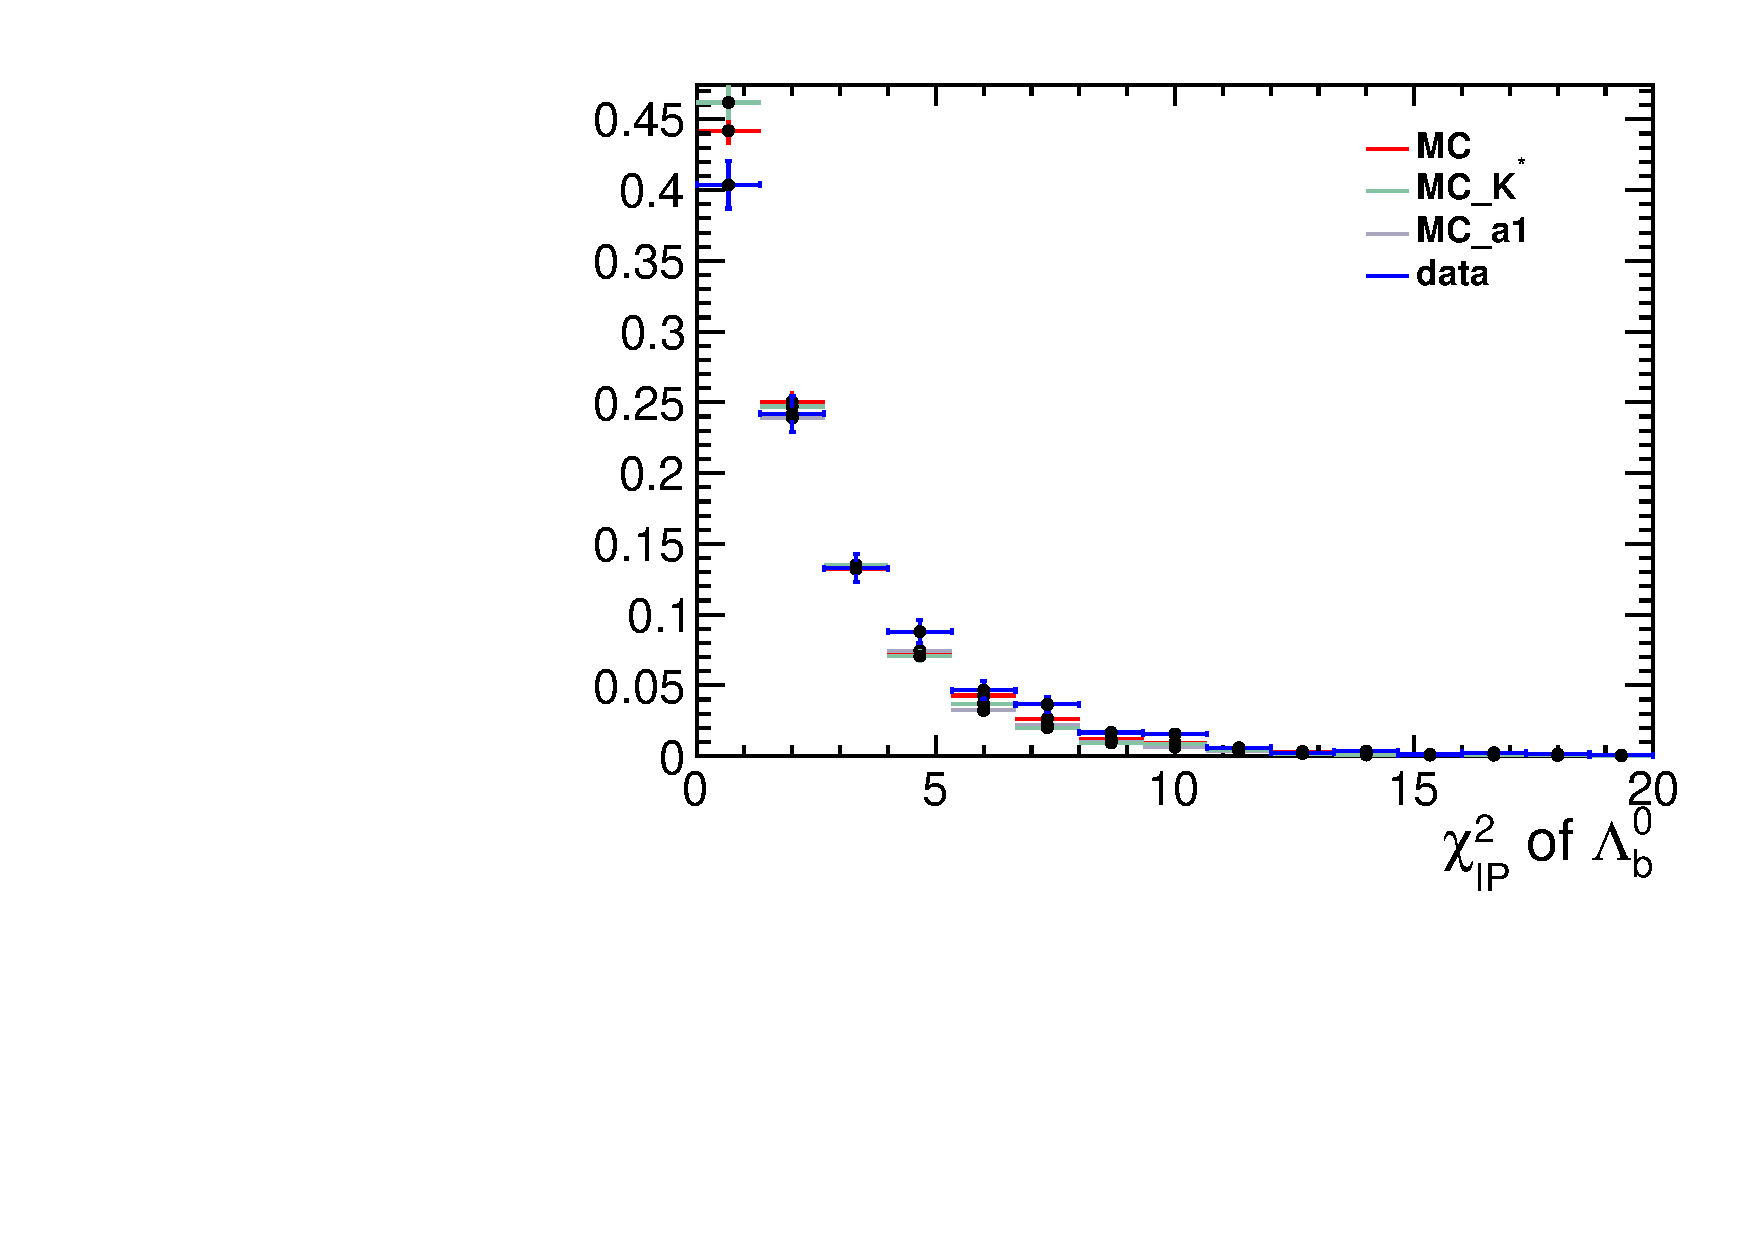
\includegraphics[width=0.4\textwidth]{Figures/05_open_charm/04_tune/Lckkpi_smear/before/Lb_IPCHI2_OWNPV.pdf}%
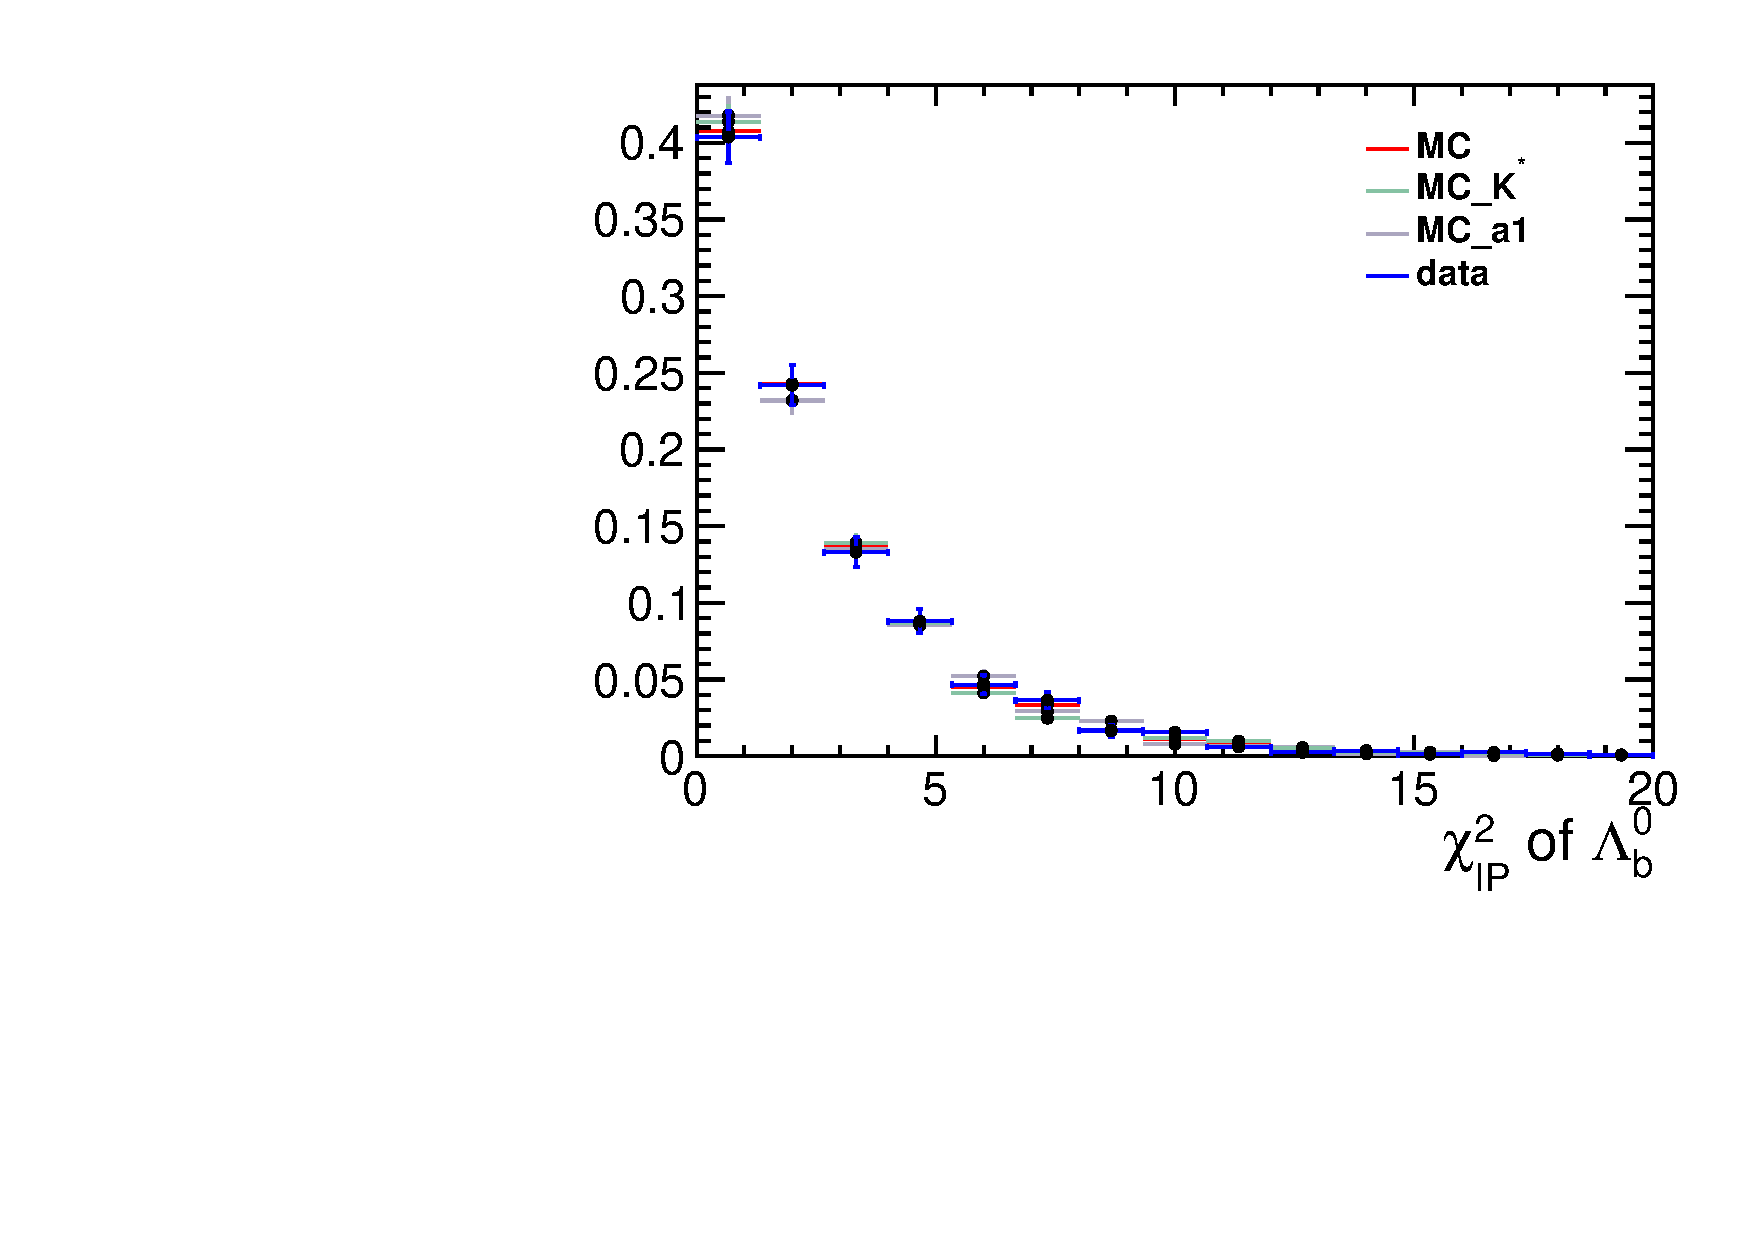
\includegraphics[width=0.4\textwidth]{Figures/05_open_charm/04_tune/Lckkpi_smear/after/Lb_IPCHI2_OWNPV.pdf}\\%
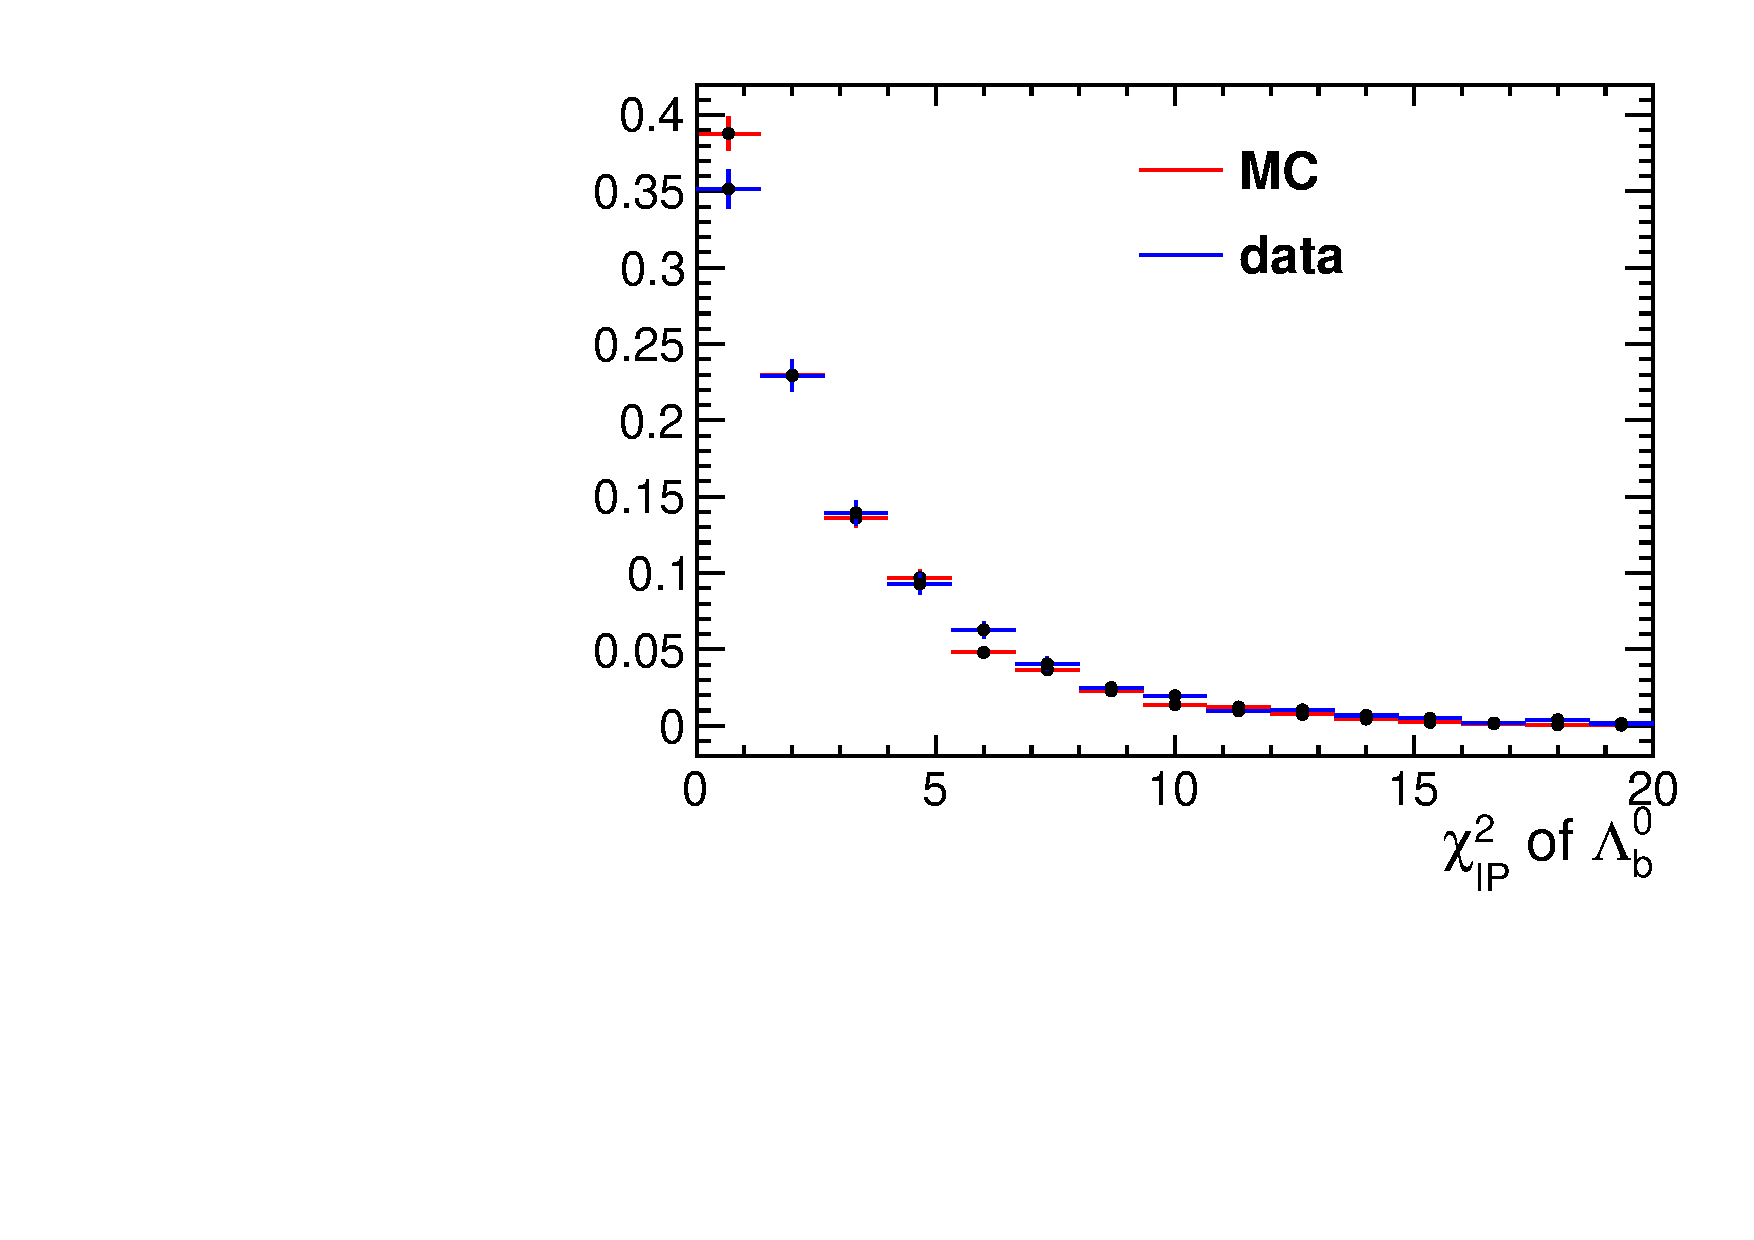
\includegraphics[width=0.4\textwidth]{Figures/05_open_charm/04_tune/LcDs_smear/before/Lb_IPCHI2_OWNPV.pdf}
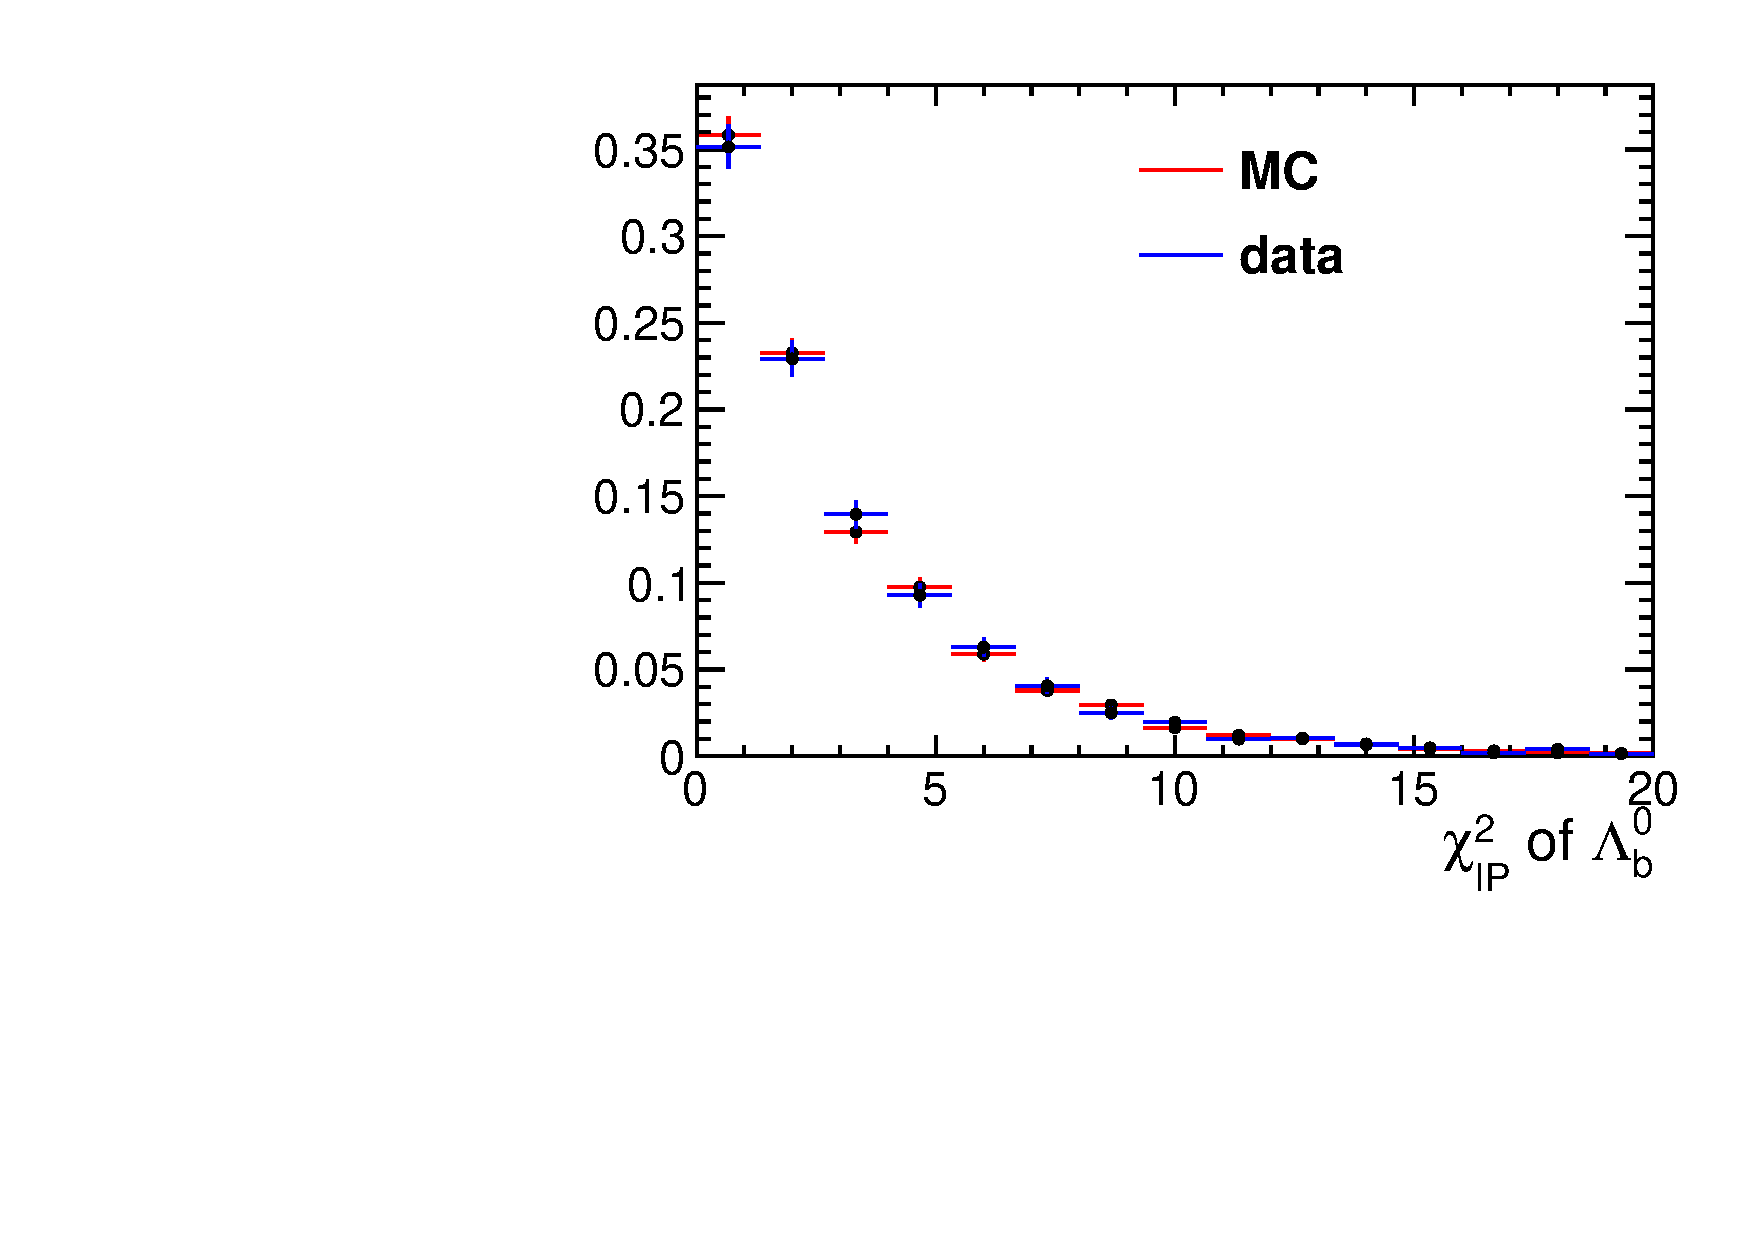
\includegraphics[width=0.4\textwidth]{Figures/05_open_charm/04_tune/LcDs_smear/after/Lb_IPCHI2_OWNPV.pdf}
\caption{The comparison of background subtracted data and signal MC for and \LbLckkpi(top) and \LbLcDs(bottom), and the s-plot method is used to get the background subtracted data. The red line is the MC signal and blue is data. Left is the distribution before smearing and Right is after smearing.}
\label{Fig.diff_cut_value_pi}
\end{figure}

The $\chi^2_{\rm IP}$ of the final state tracks and $\Lb$ is different in the background subtracted data and signal MC  
in \LbLcDs and in \LbLckkpi(as shown in Figure.~\ref{Fig.diff_cut_value_pi}). 
We smeared the distributions of these variables and the distribution after smearing are listed in the right of Figure.~\ref{Fig.diff_cut_value_pi}, 
and generating gaussian random numbers to get $\chi^2$ distributed variables. 
As for \LbLckkpi, the same smearing are applied to the MC sample.


The distribution of variables used in TMVA, 
$\chi^2_{\rm IP}$ of the final tracks need to be tuned. 
%as shown in the Appendix.~\ref{appendix:IPsmearing}.  
And other variables that are used in the cut have consistent distributions between data and MC.

\subsection{$\pt, ~y$, nTracks reweight}
\label{sec:getptyweight}

In order to take into account data-MC difference, 
especially the initial kinematic of the mother particle \Lb, the MC samples need to be reweighted. 

The $\pt$, rapidity $y$ and nTracks weight is obtained from the normalization channel \LbLcDs  with \Lb Global(TOS) requirement 
and apply the weights to both \LbLckkpi and \LbLcDs samples. 
As the $\pt$ and $y$ are properties of \Lb which is the same mother particle for signal channel and normalization channel, 
it should be fine to apply the weight obtained from the normalization channel to the signal channel. 
The nTracks representing the multiplicity of the event, 
and don't have large difference between the signal channel and normalization channel. 
Beside, 
we have considered the track correction, trigger, PID efficiency in the Monta Carlo sample before applying \pt, y weight. 

We weight the $\pt$,$y$ at the same time, 
and then apply a nTracks weight, because the statistics is limited to use a 3-D weight. 
The transverse momentum and rapidity of \Lb are compared between the data sample after background with the sPlot technique and the MC sample. 
The ratio between data and MC distribution in the two dimensions is taken as weights, 
as shown in Figure.~\ref{Fig.pt_y_ratio}. 
%More plots about the distributions before and after reweight are shown in Appendix.~\ref{appendix:check}.

\begin{figure}[bth]
\centering
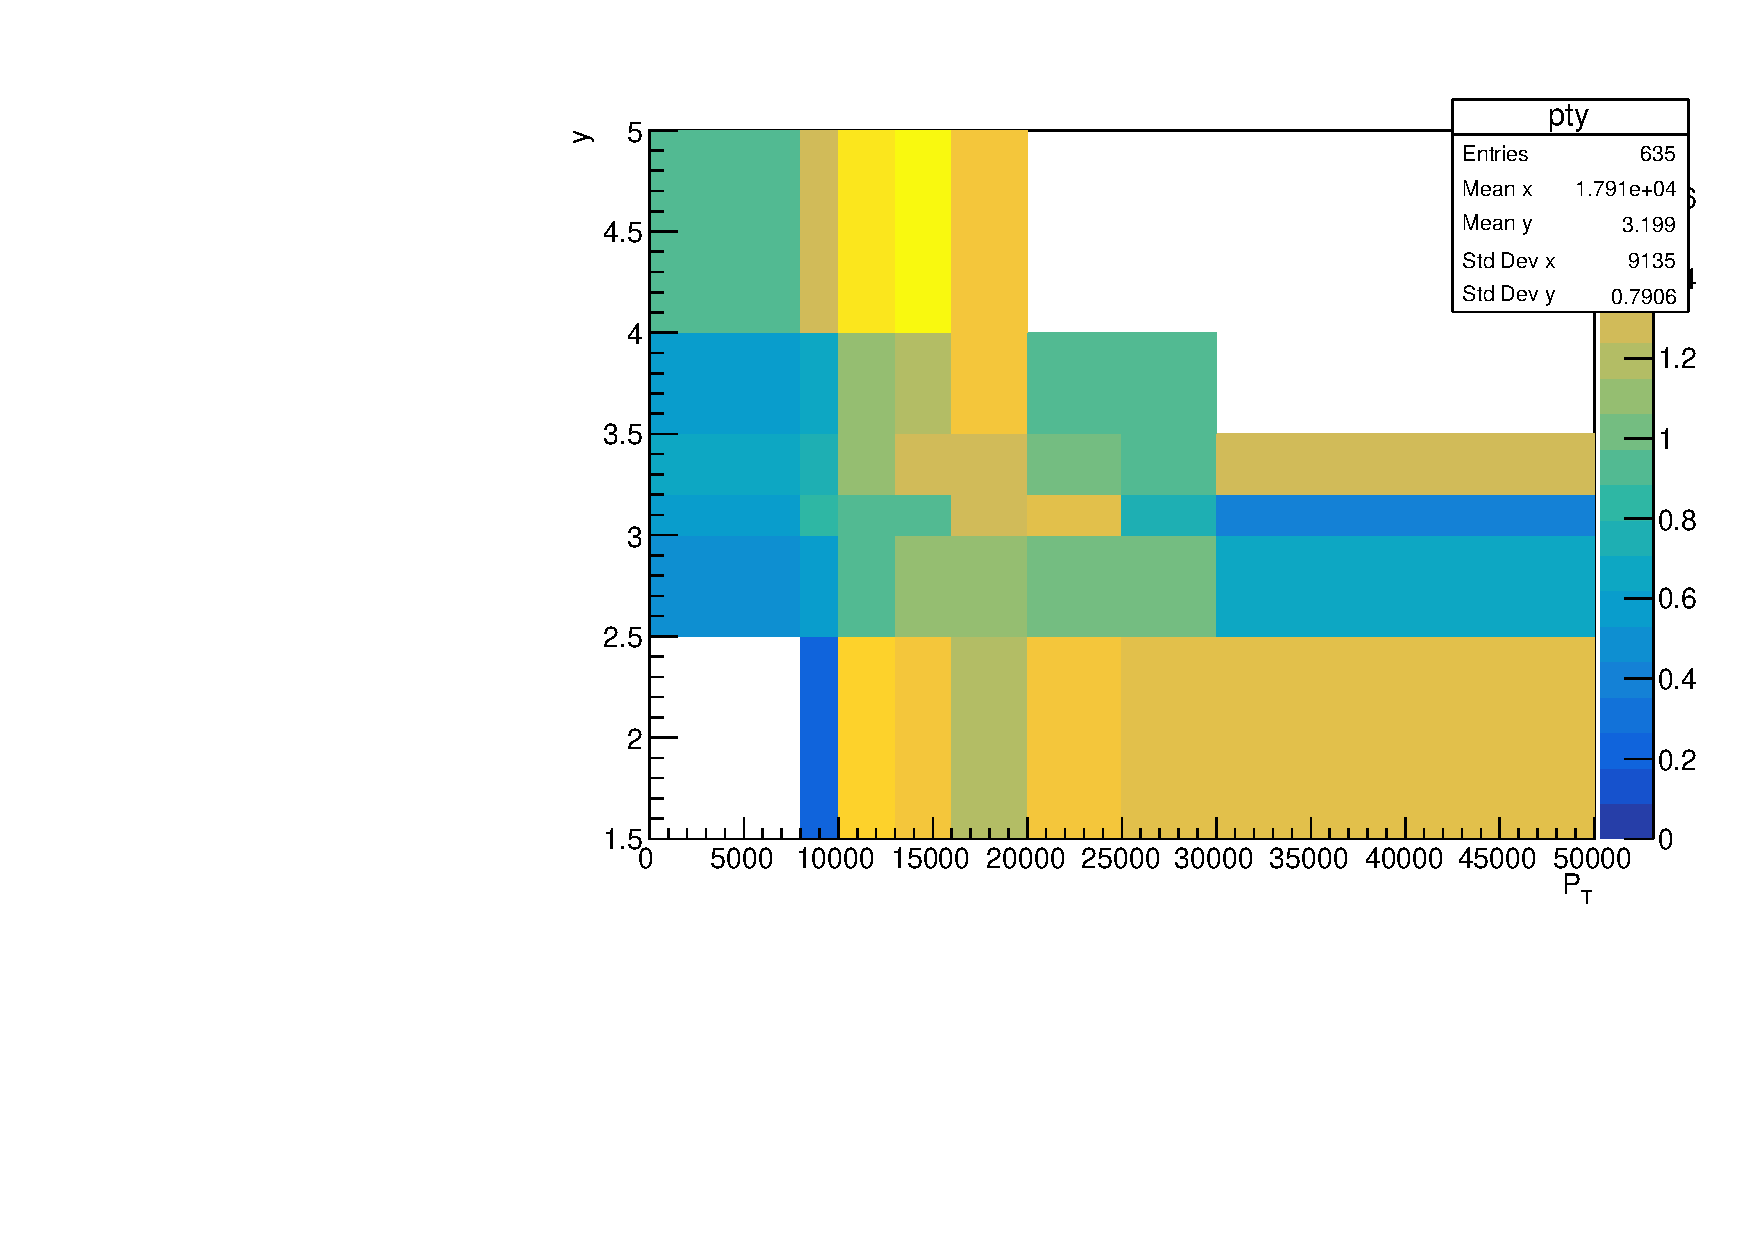
\includegraphics[width=0.4\textwidth]{Figures/05_open_charm/04_tune/pt_y/ratio_pty.pdf}%
	\caption{ Relative yields between background-subtracted data and signal MC of \LbLcpi as function of $\pt$ and $y$ of \Lb baryons. 
	The relative yield in each bin is shown with the color sized Z axis, and it's larger when it goes yellow.}
\label{Fig.pt_y_ratio}
\end{figure}

There's some difference between the distribution of multiplicity in background subtracted data and signal MC. 
And when estimating the PID efficiencies, the nTracks are used. 
We reweighted the distribution of MC to be the same as real data. 
We generate the weight tables of signal channel and normalization channel using \LbLcDs sample. 

\subsection{\Lc Dalitz reweight}
\label{sec:getdalitzweight}

The description of \Lc decays in simulated events can be different from the real situation. 
Since the MC have different \Lc decays in the signal and normalization channels, 
separate weights are obtained. 
For normalization channel, 
the statistics of data and MC are both large, 
so we apply a 2-D Dalitz reweight so that the MC distribution is consistent with data. 
The comparison between MC and data for normalization channel is shown in Figure.~\ref{Fig.dalitz_distri_pi}.

\begin{figure}[bth]
\centering
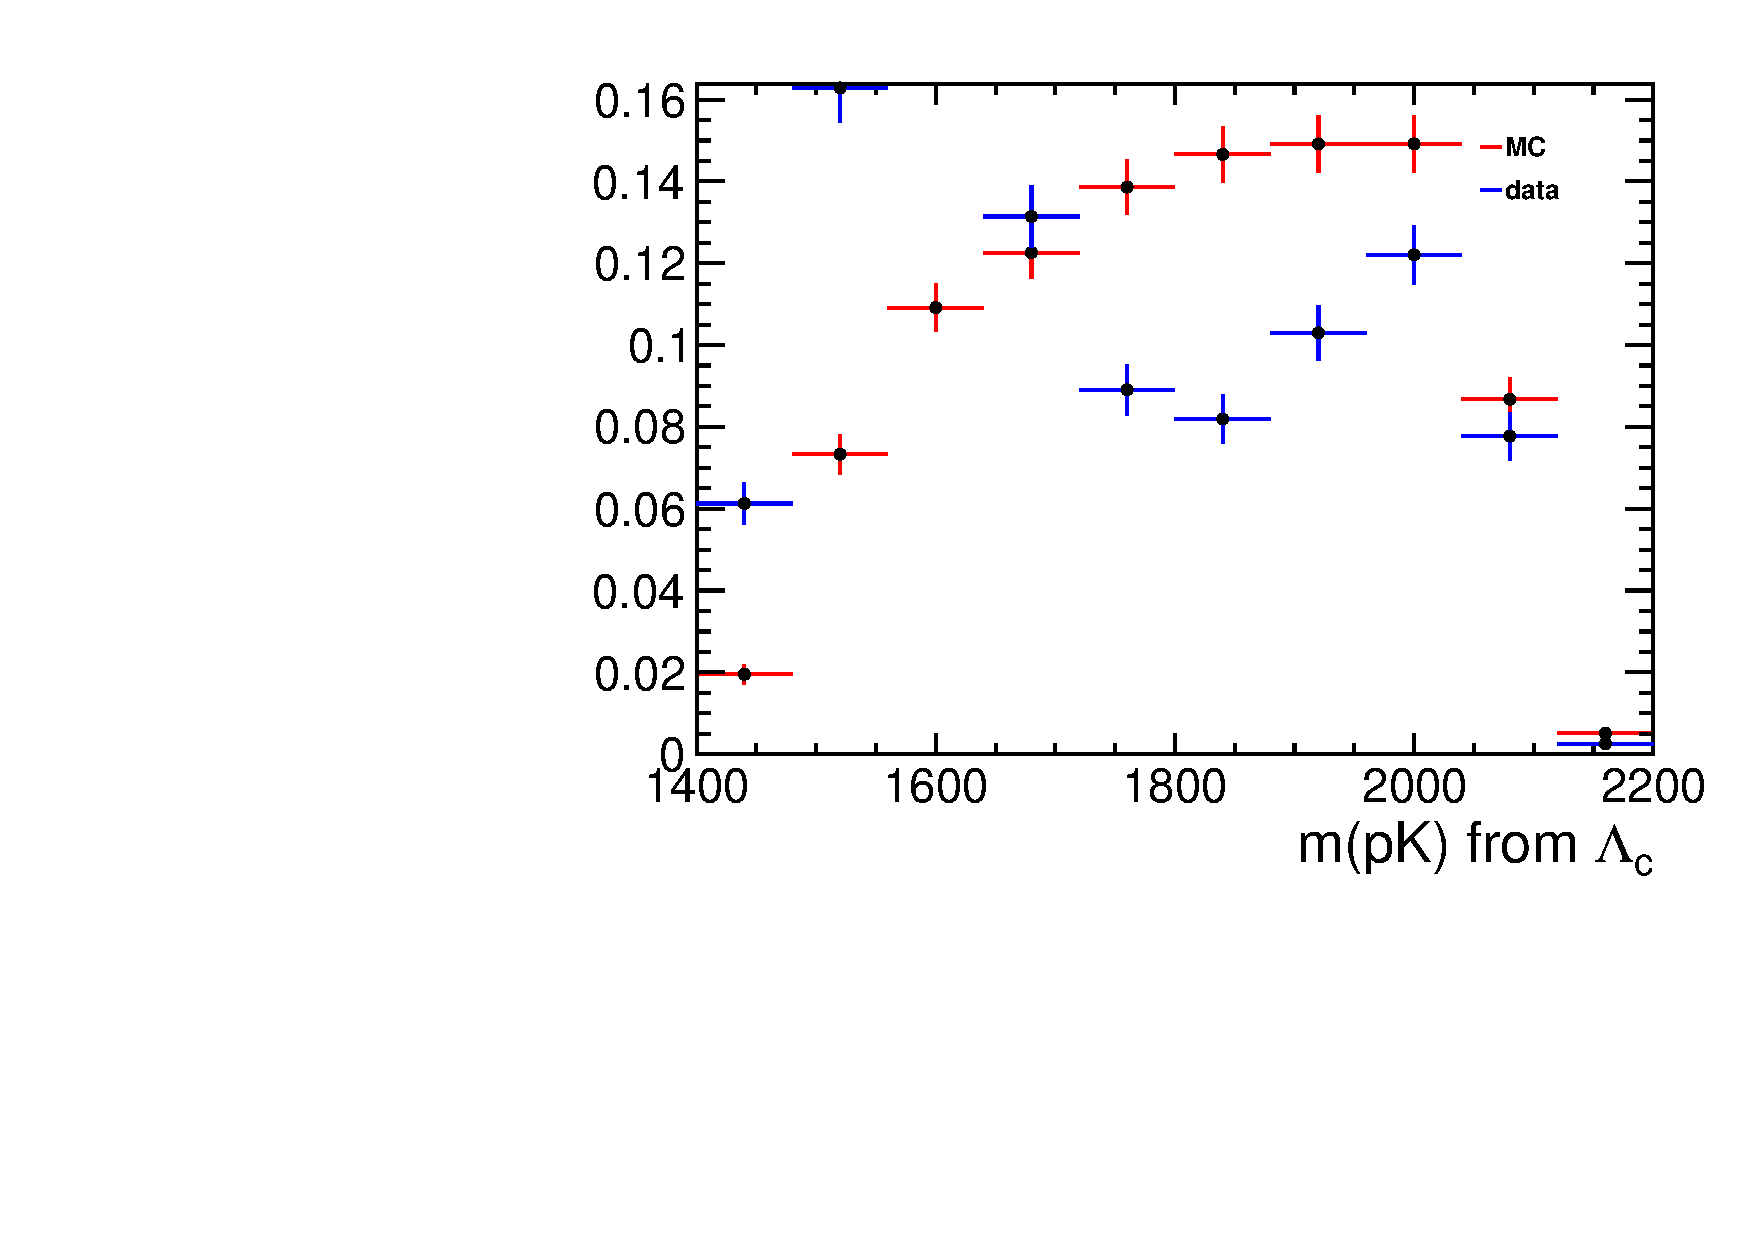
\includegraphics[width=0.4\textwidth]{Figures/05_open_charm/04_tune/dalitz/mkp.pdf}%
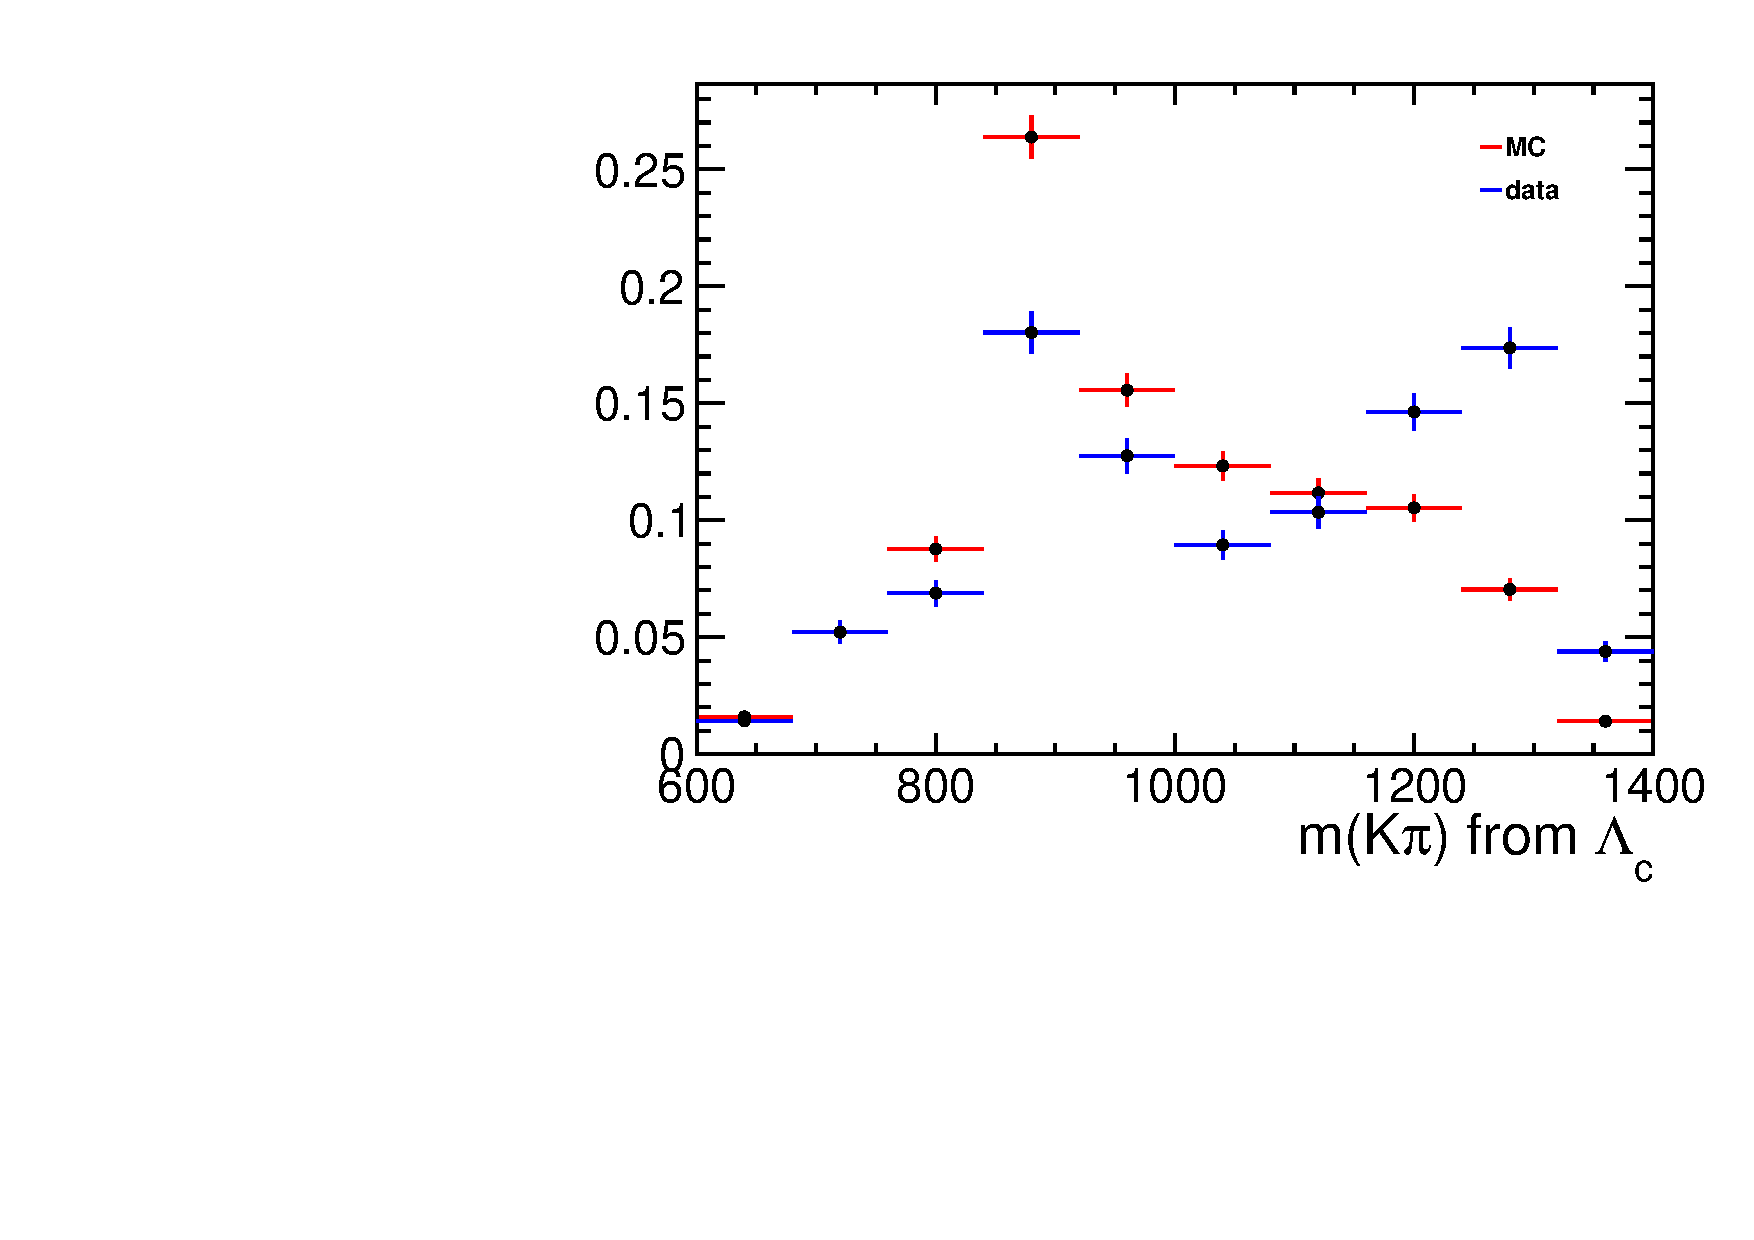
\includegraphics[width=0.4\textwidth]{Figures/05_open_charm/04_tune/dalitz/mkpi.pdf}%
\caption{ The distribution of invariant mass of combination of \Lc daughters in \LbLcDs channel}
\label{Fig.dalitz_distri_pi}
\end{figure}

\begin{figure}[bth]
\centering
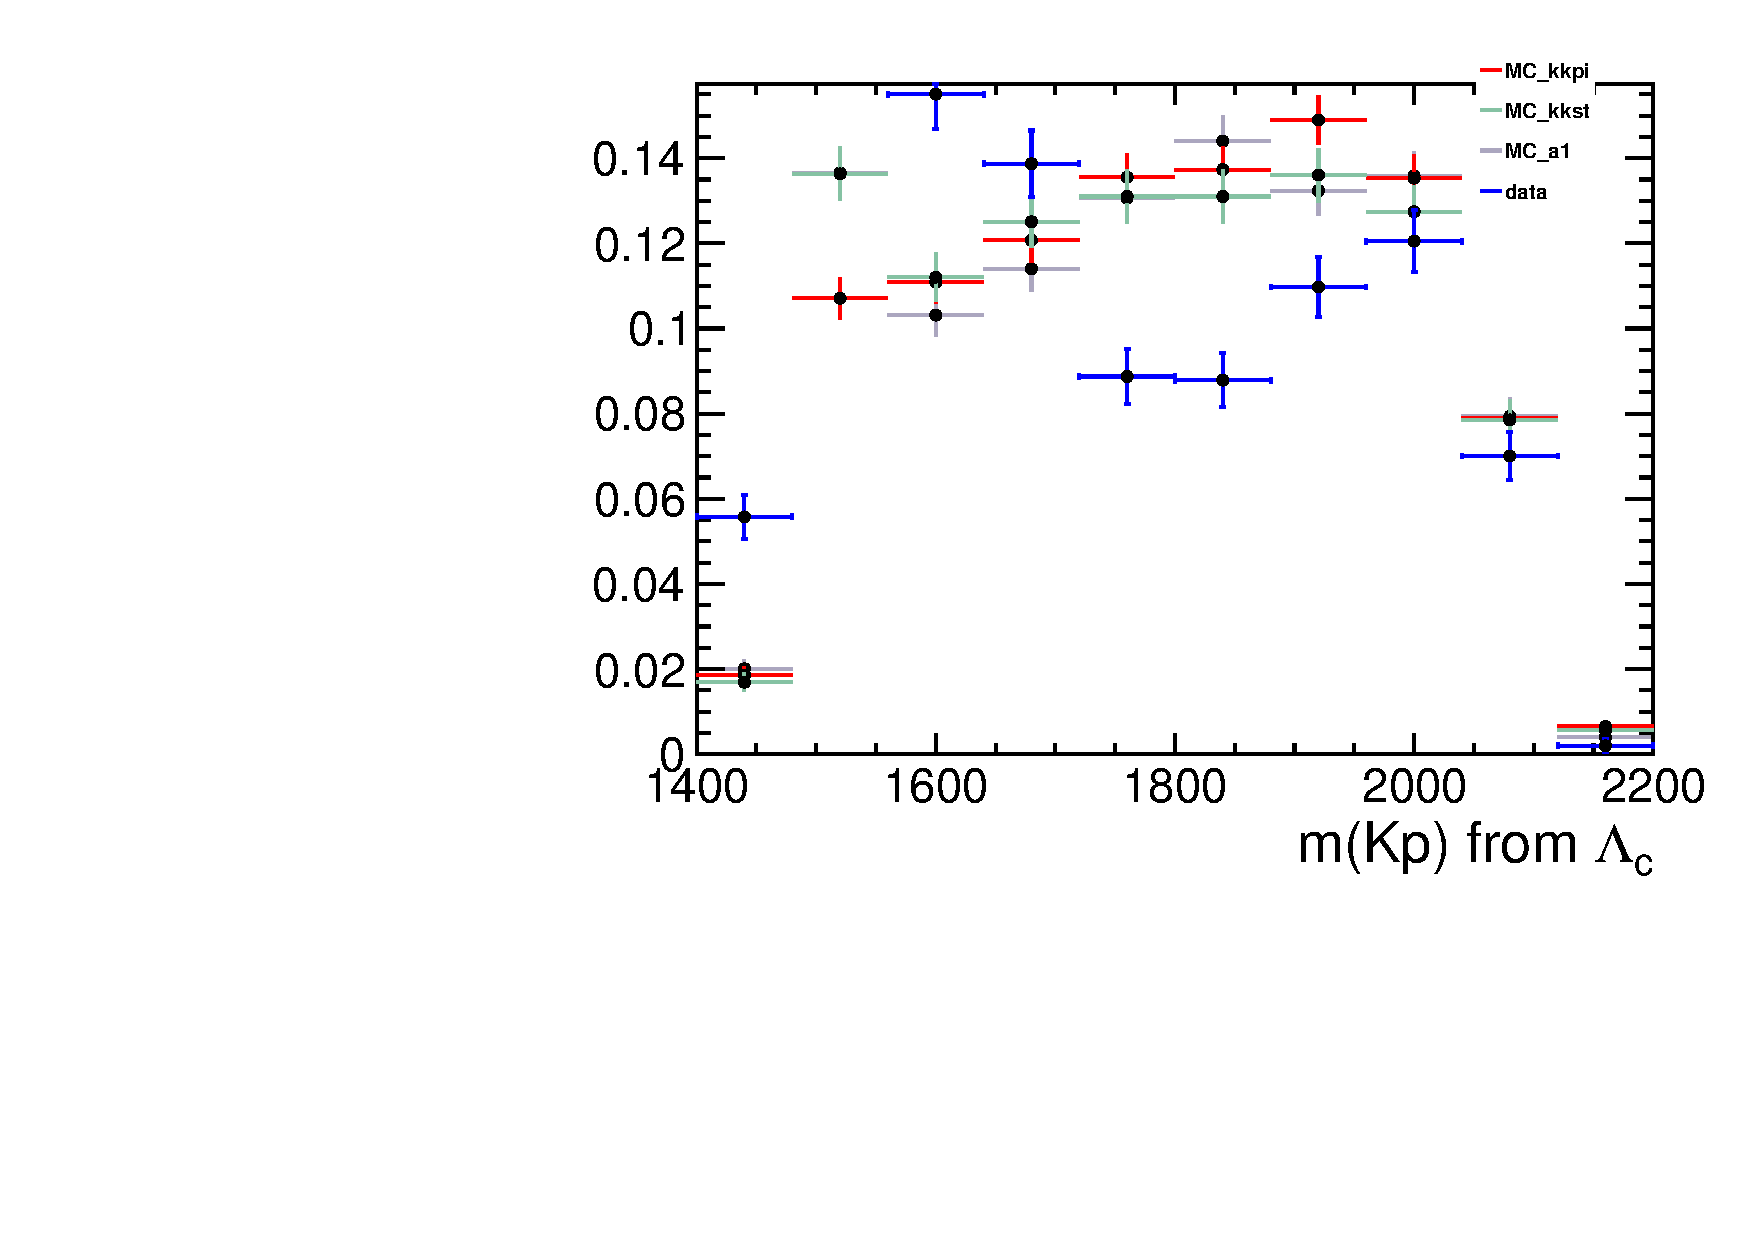
\includegraphics[width=0.4\textwidth]{Figures/05_open_charm/04_tune/dalitz/signal_channel/mkp.pdf}%
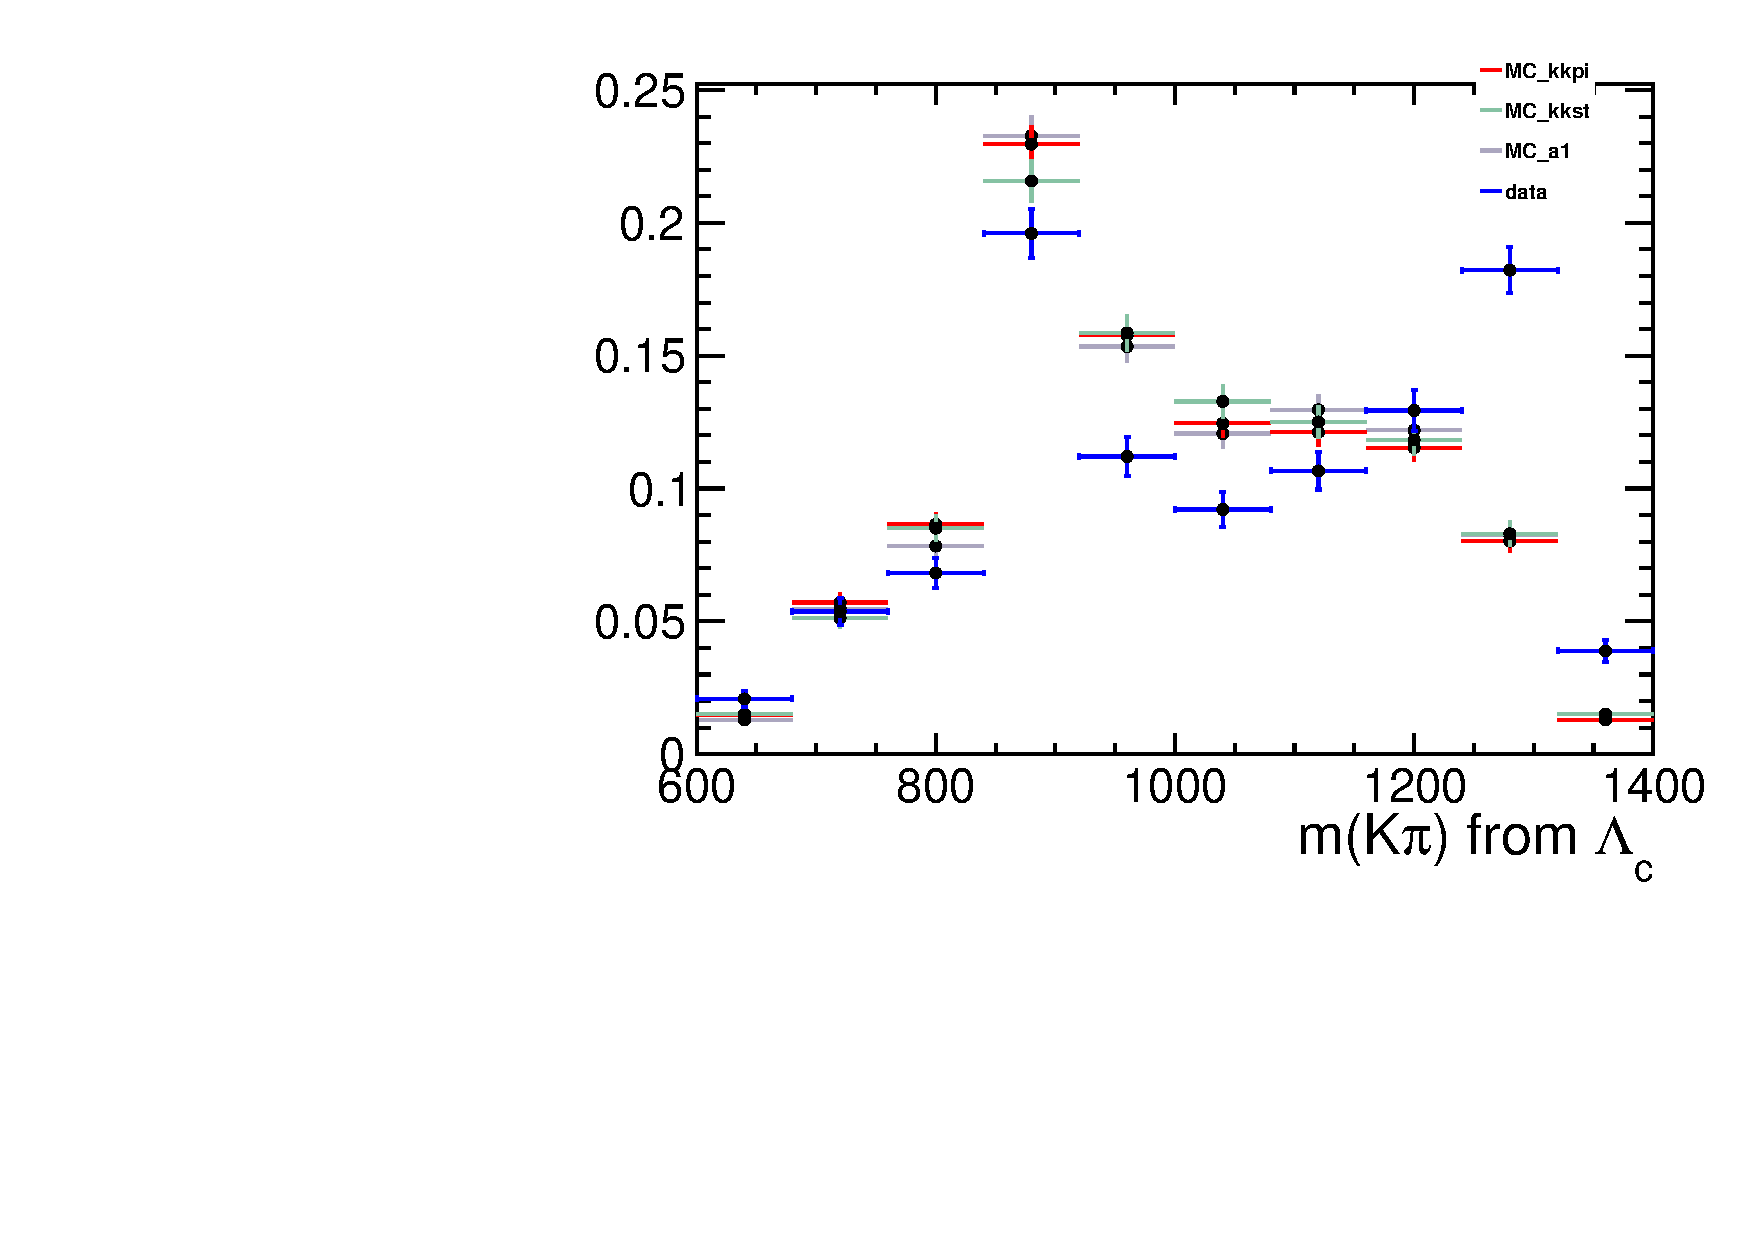
\includegraphics[width=0.4\textwidth]{Figures/05_open_charm/04_tune/dalitz/signal_channel/mkpi.pdf}%
\caption{ The distribution of invariant mass of combination of \Lc daughters in \LbLckkpi channel}
\label{Fig.dalitz_distri_kkpi}
\end{figure}


For the signal channel, the same method is used. 
Because the statistics of the data is limited for signal channel, 
the bin width is larger than that used in the normalization channel. 
Figure~\ref{Fig.dalitz_distri_kkpi} shows the comparison between data and MC for invariant mass distributions of $pK$ and $\pi K$. 
The weights for these two channels are shown in Figure.~\ref{Fig.dalitz_ratio}. 
Then these weights are applied to our MC samples both in reconstruction and generator level.

\begin{figure}[bth]
\centering
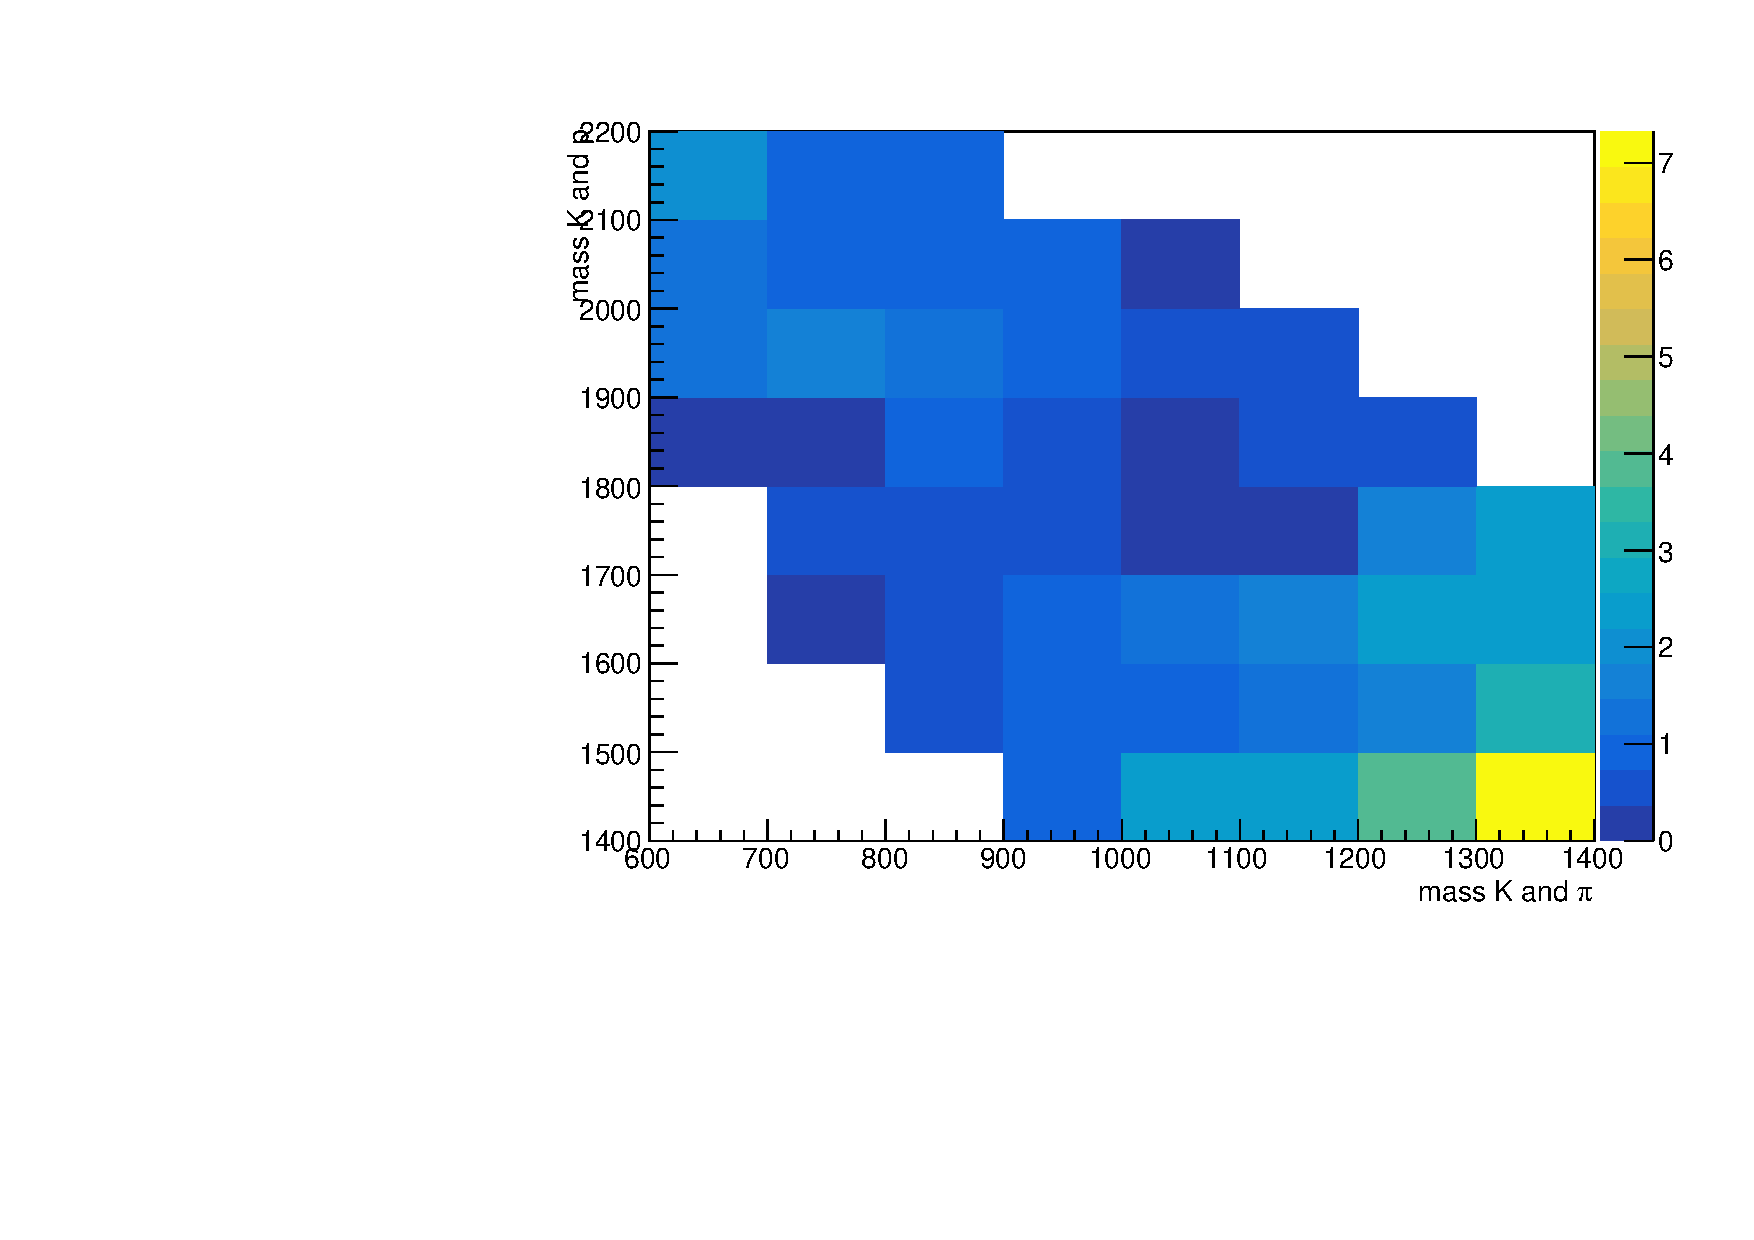
\includegraphics[width=0.4\textwidth]{Figures/05_open_charm/04_tune/dalitz/ratio_dalitz_ds.pdf}%
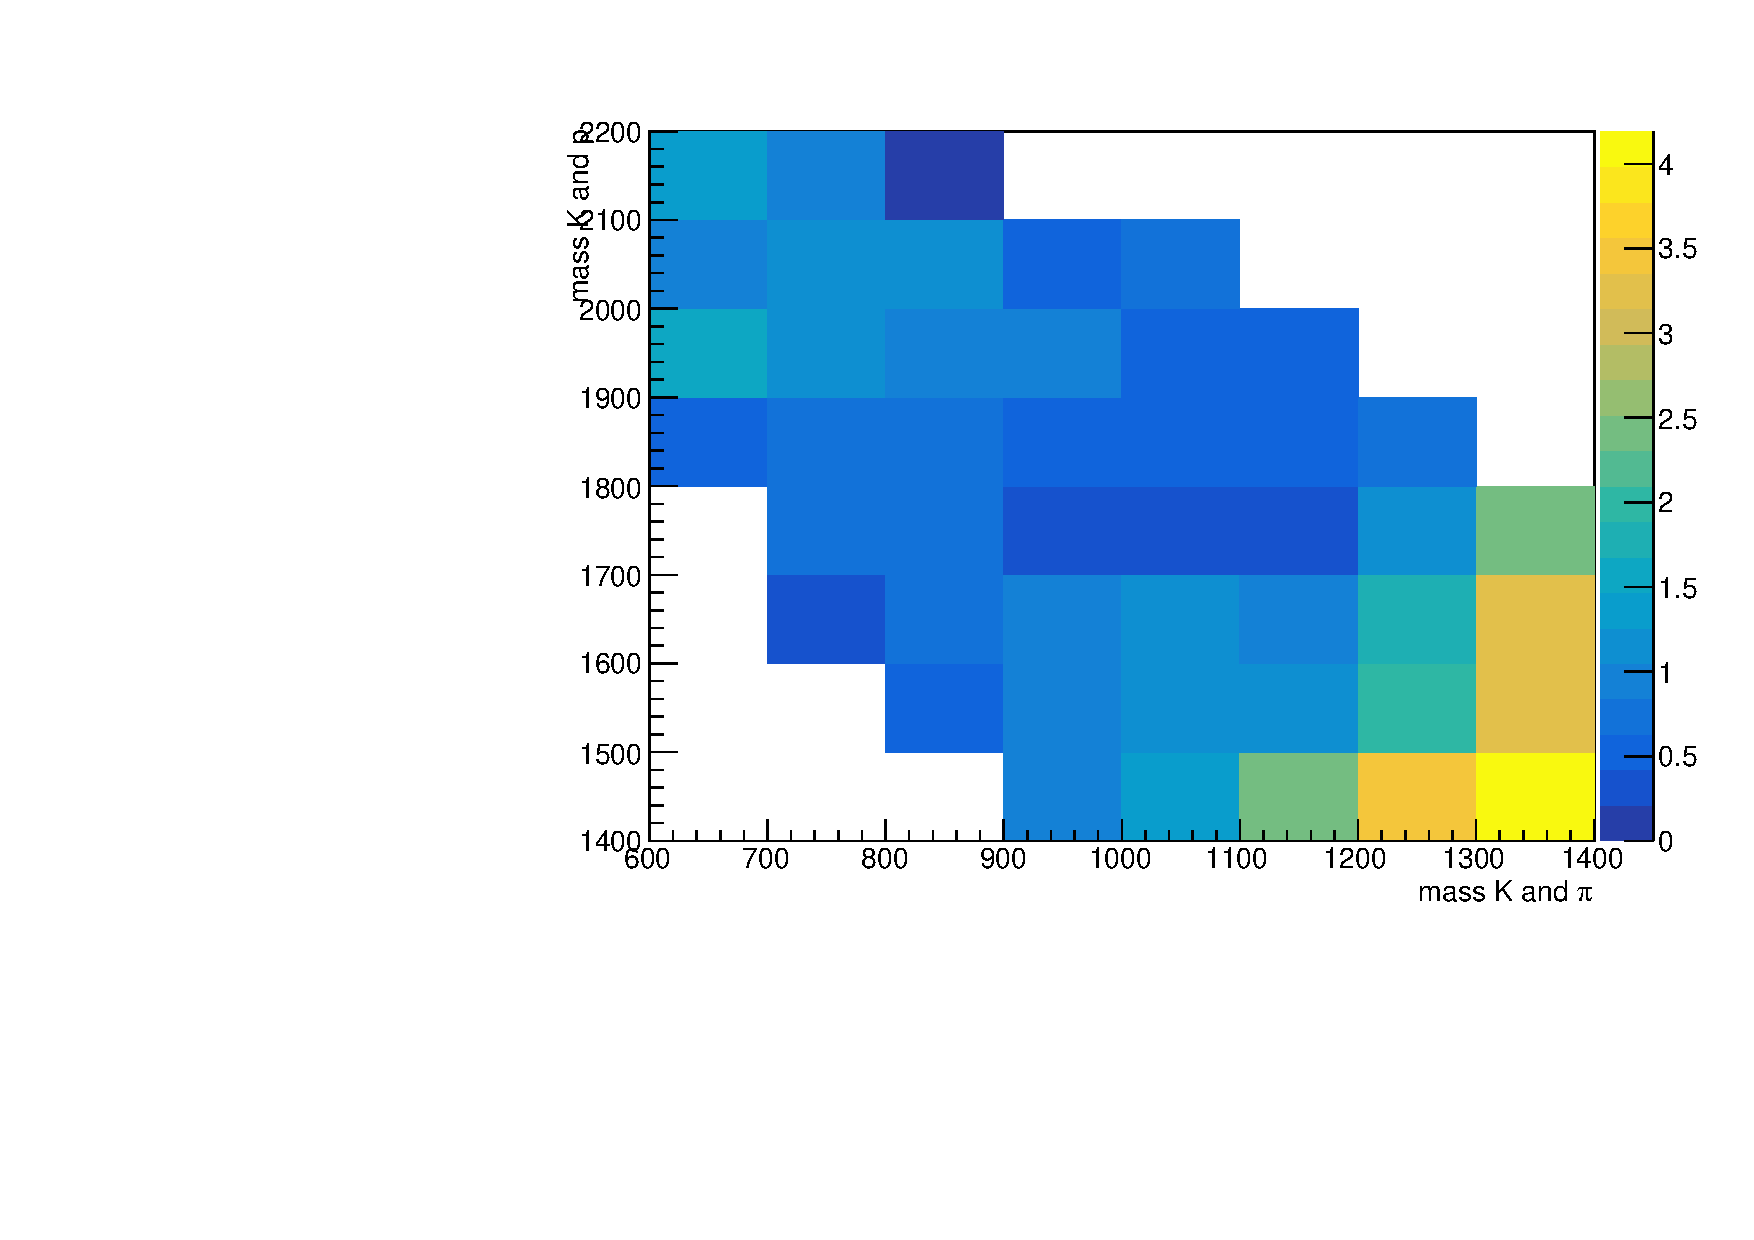
\includegraphics[width=0.4\textwidth]{Figures/05_open_charm/04_tune/dalitz/ratio_dalitz_kkpi.pdf}%
	\caption{ The distribution of combination invariable mass of \Lc daughters in \LbLcDs channel (left) and \LbLckkpi channel (right)}
\label{Fig.dalitz_ratio}
\end{figure}


\subsection{\Lc polarization}
\label{sec:getpoliweight}


\begin{figure}[bth]
\centering
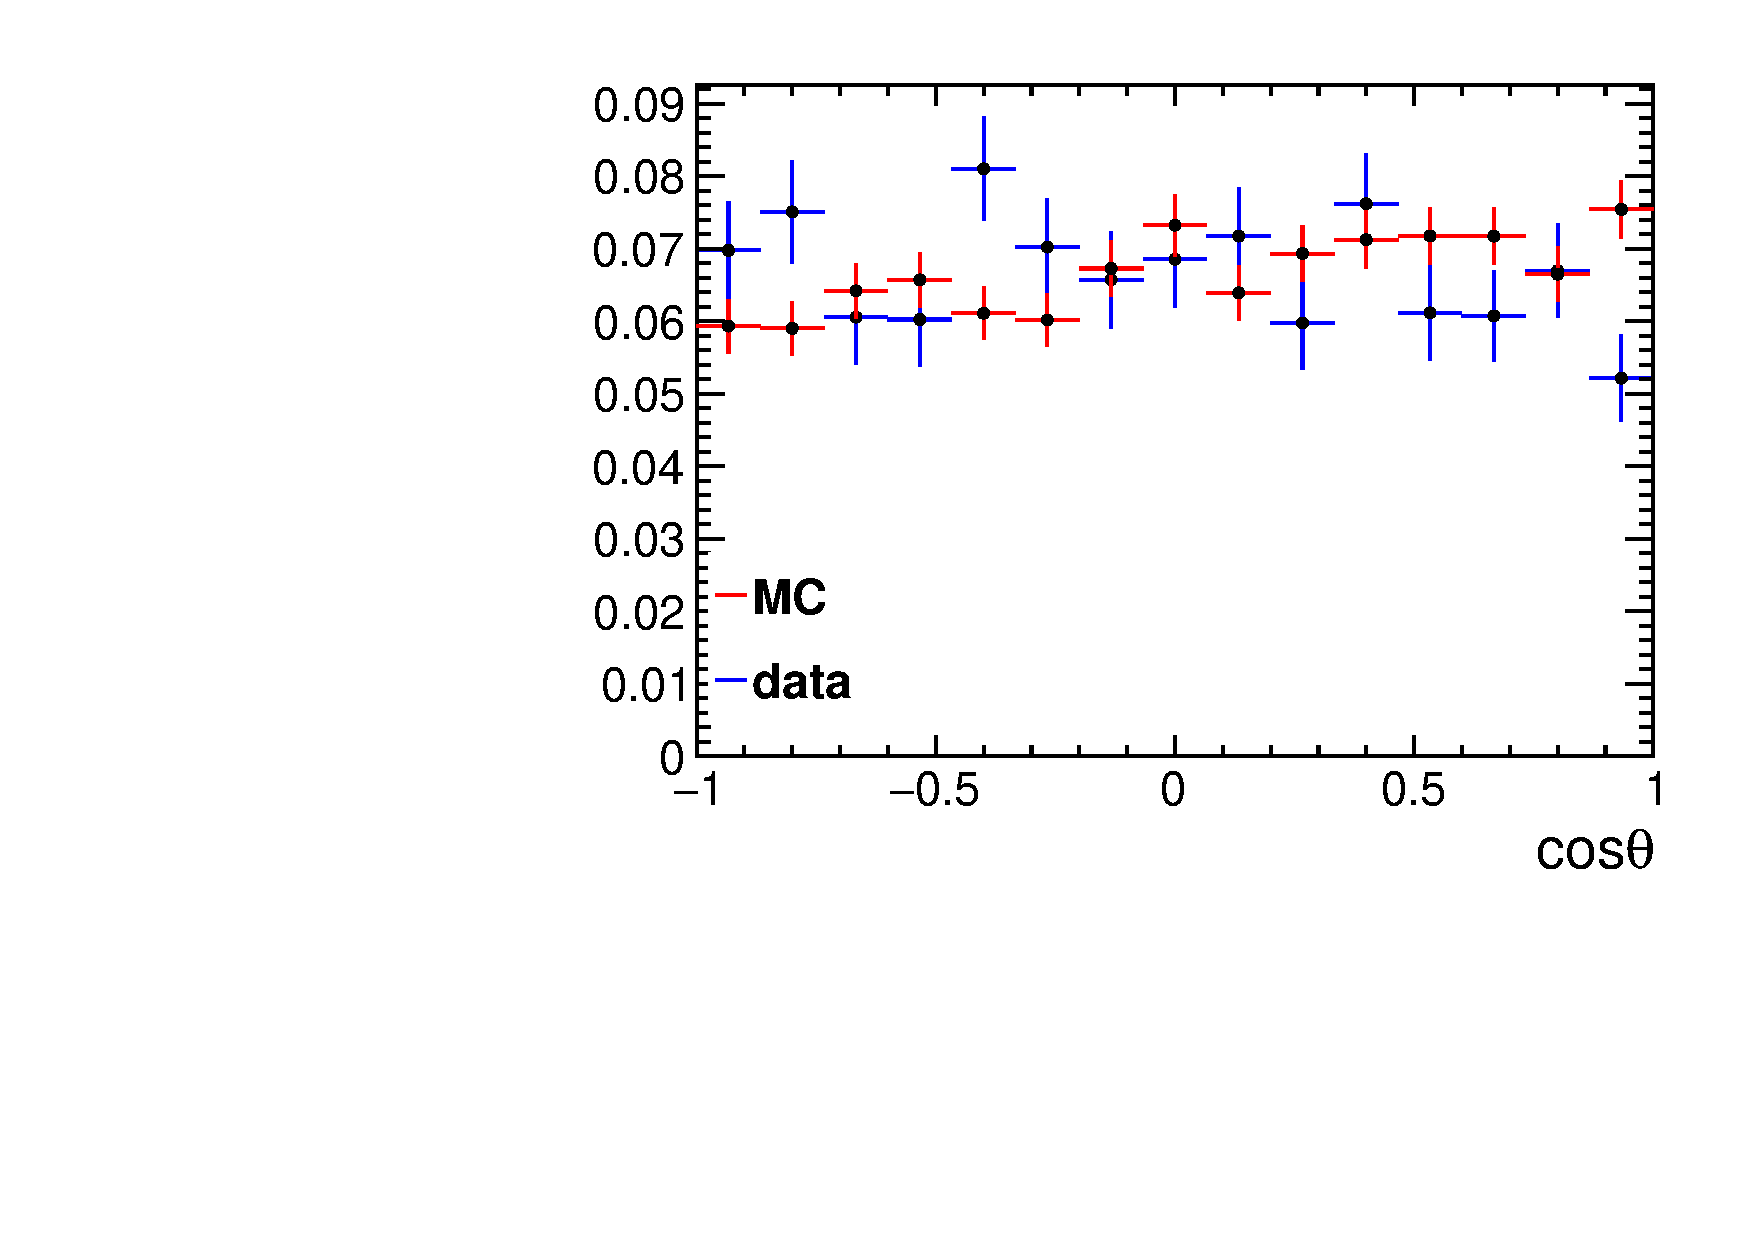
\includegraphics[width=0.4\textwidth]{Figures/05_open_charm/04_tune/poli/pi_poli/cosTheta.pdf}%
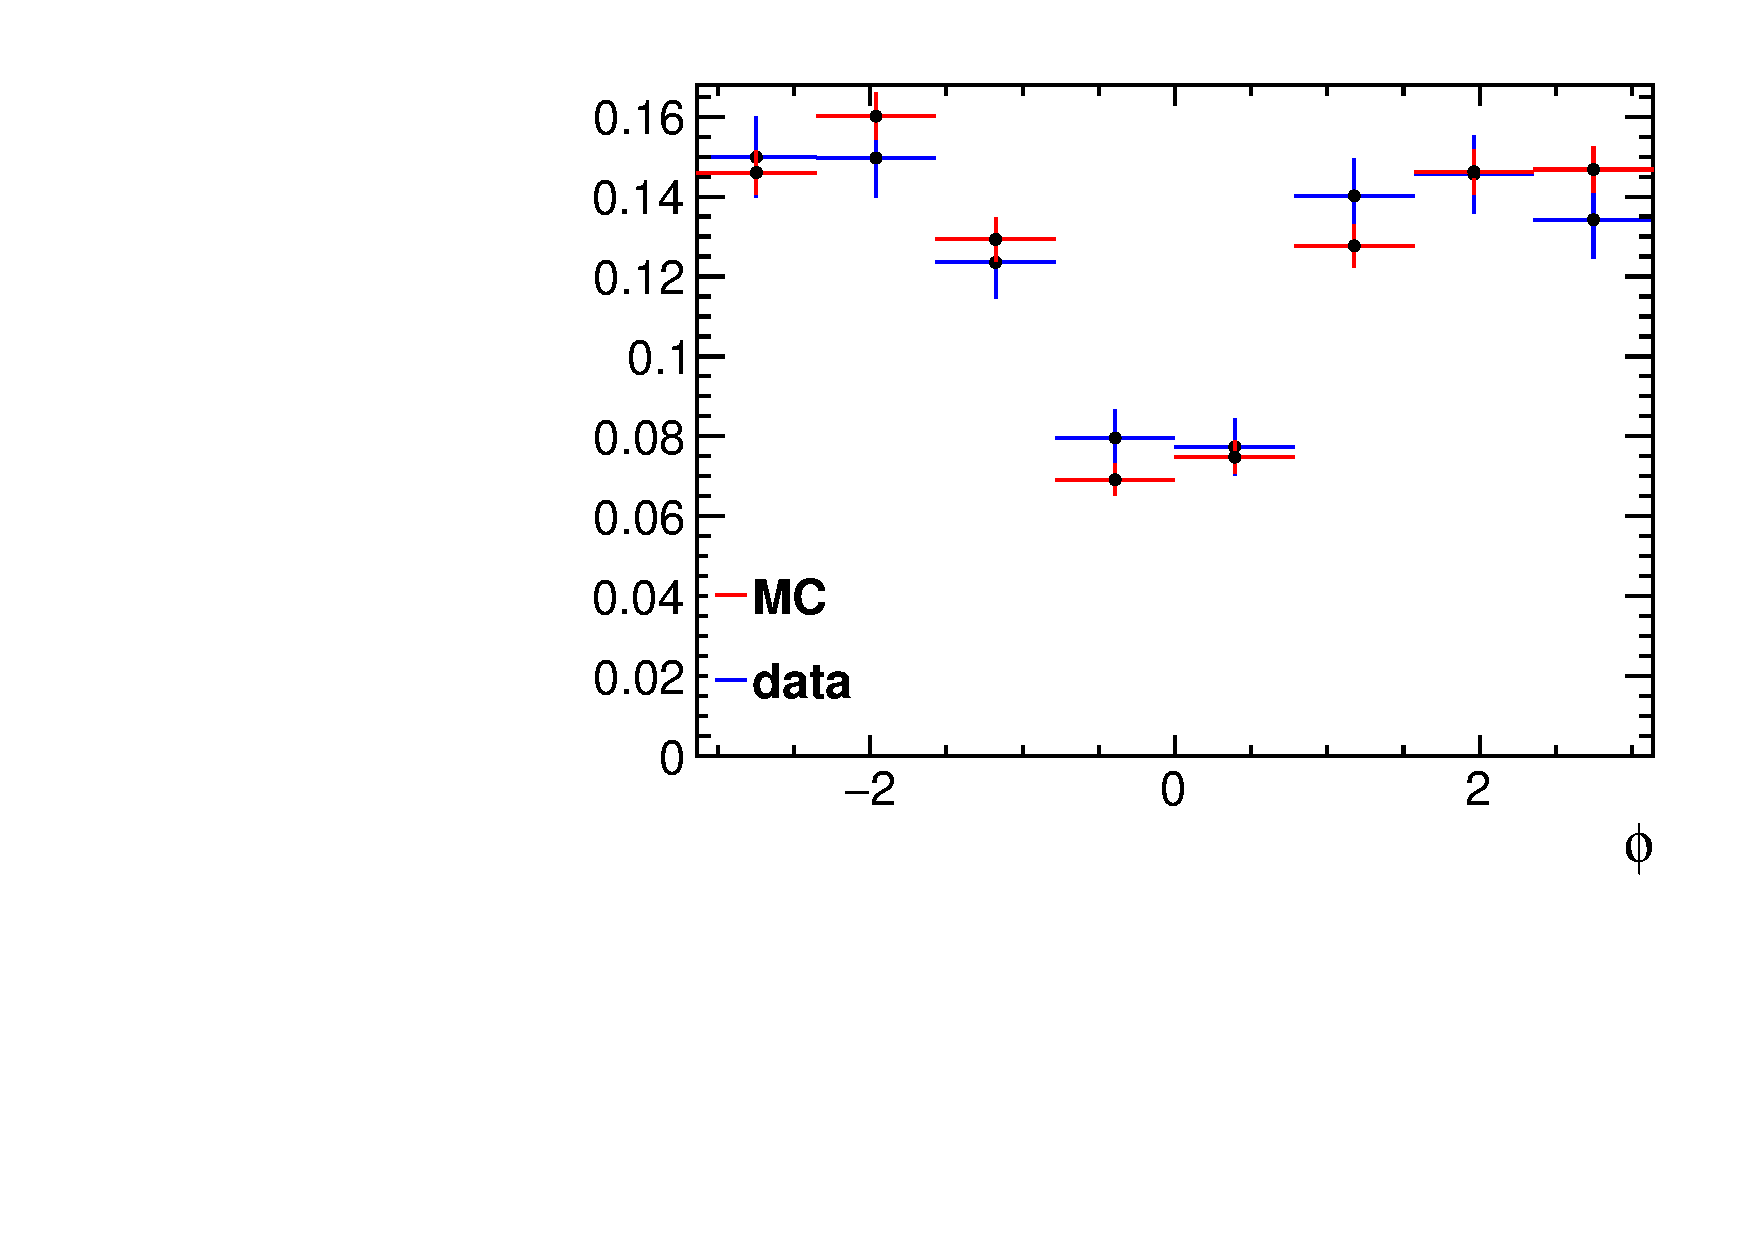
\includegraphics[width=0.4\textwidth]{Figures/05_open_charm/04_tune/poli/pi_poli/phi.pdf}\\
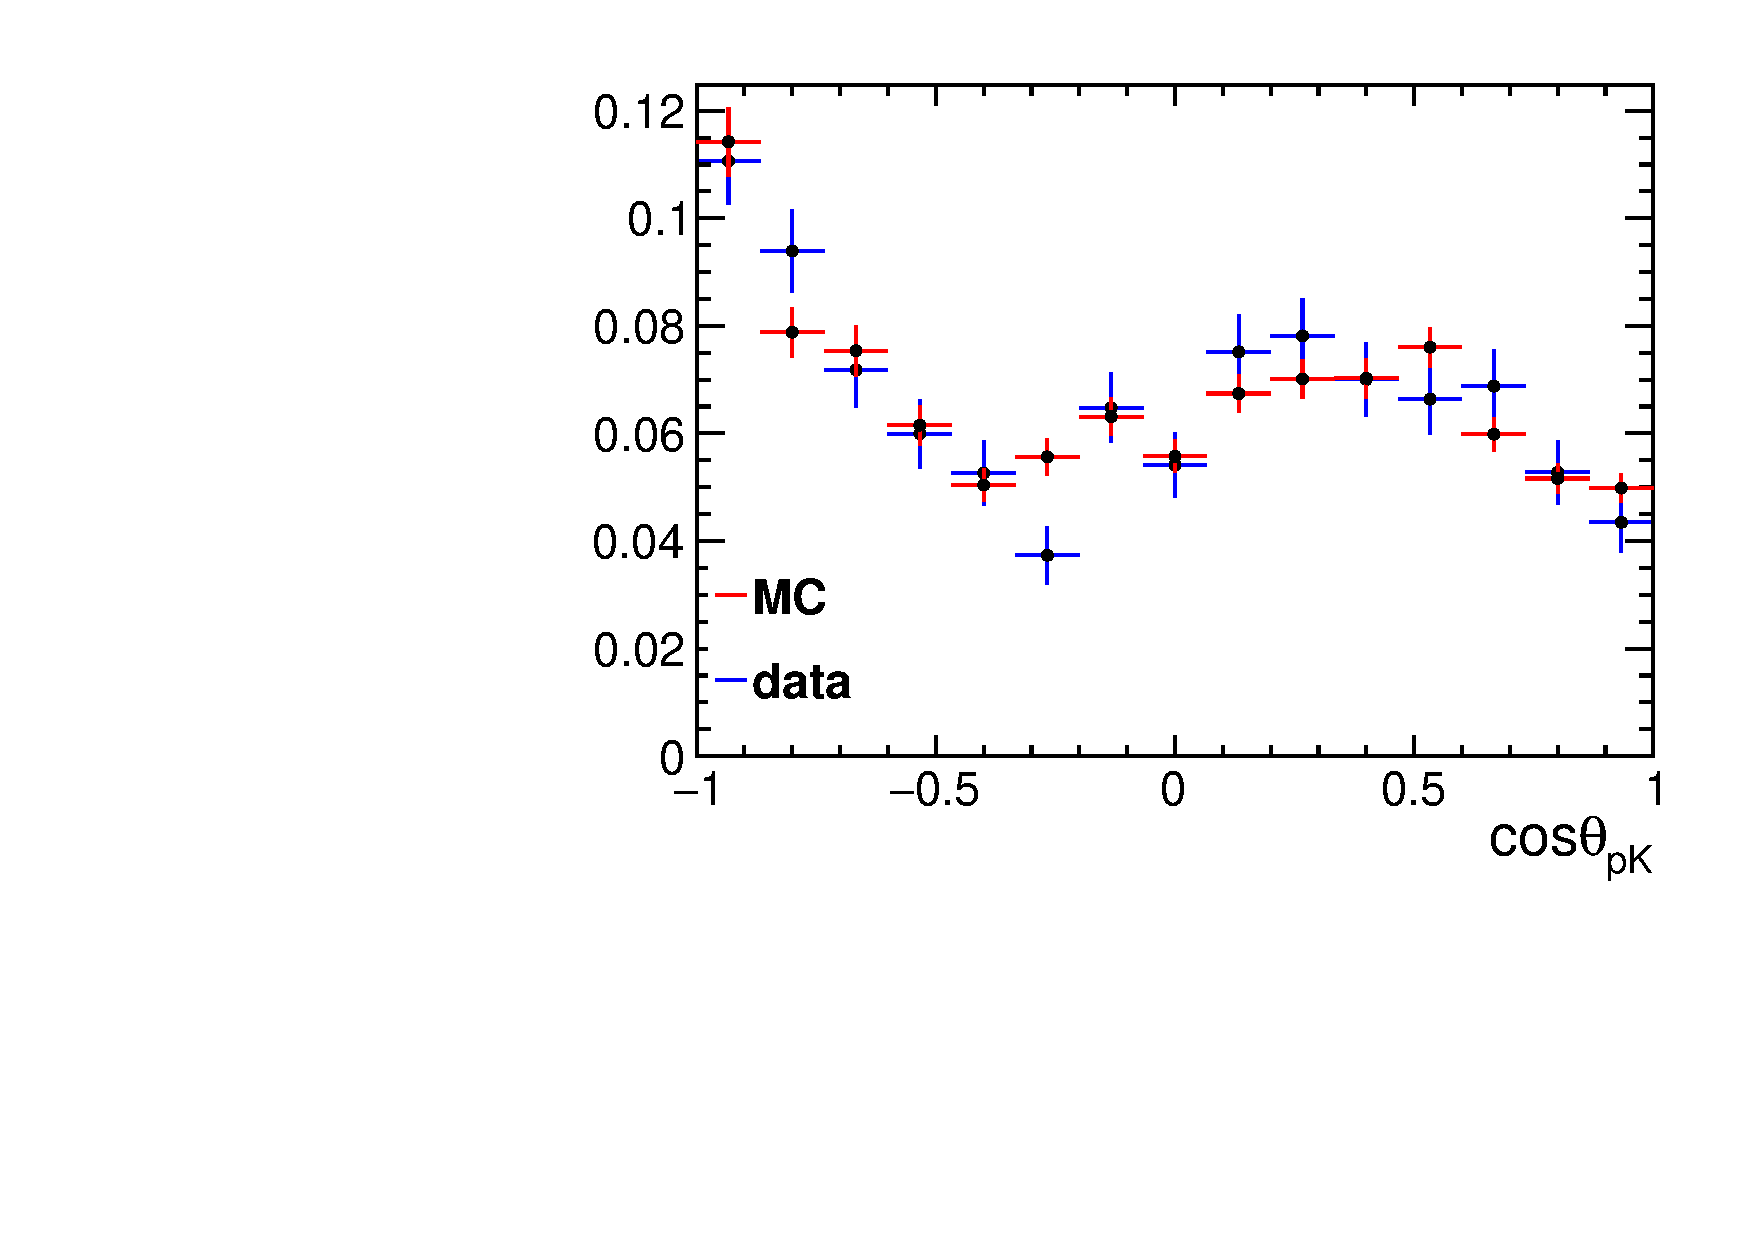
\includegraphics[width=0.4\textwidth]{Figures/05_open_charm/04_tune/poli/pi_poli/cosTheta_pk.pdf}%
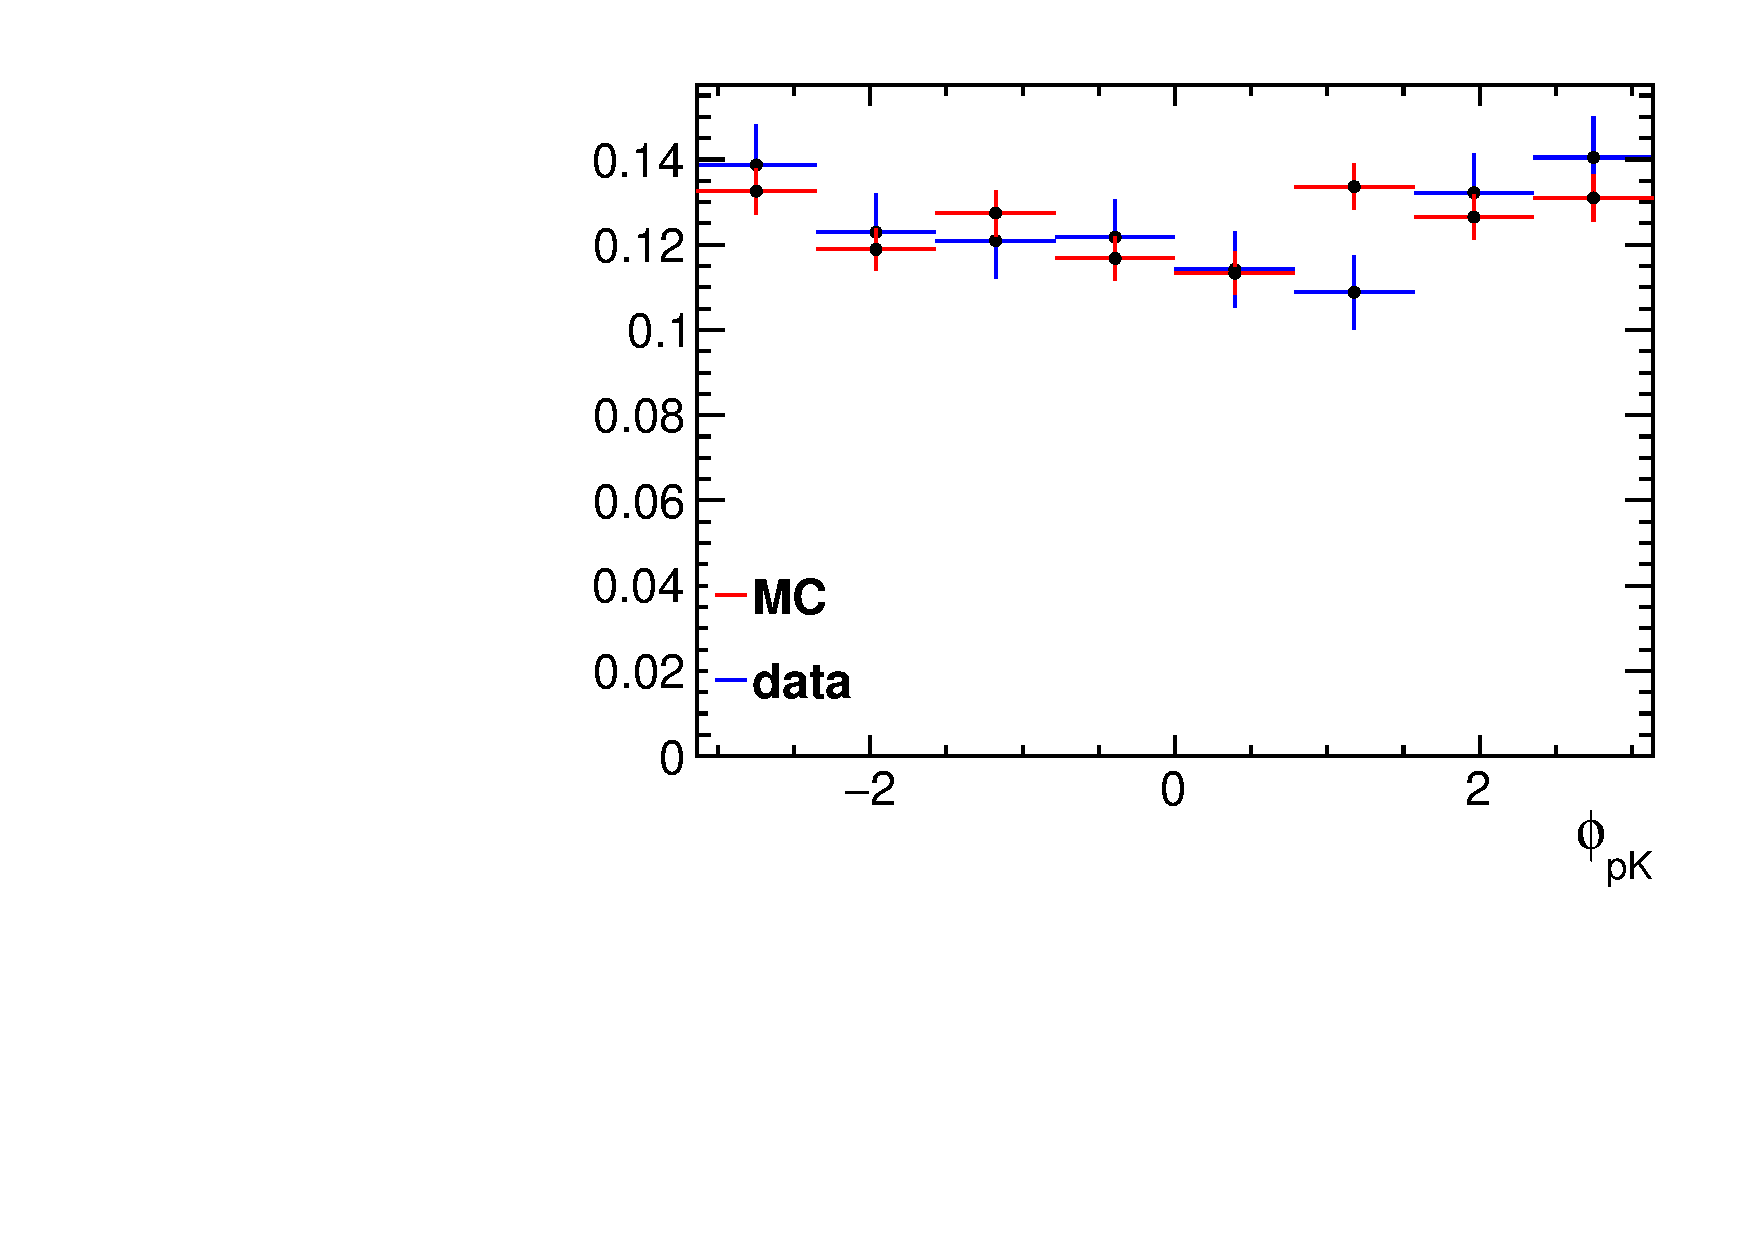
\includegraphics[width=0.4\textwidth]{Figures/05_open_charm/04_tune/poli/pi_poli/phi_pk.pdf}\\
\caption{ The distribution of some polarization angle in normalization channel}
\label{Fig.poli_pi}
\end{figure}


The polarization of \Lb is consistent with no-polarization, 
which is discussed in LHCb-ANA-2017-009, 
however, \Lc could polarized because of weak decay of \Lb. 
The MC simulation assumes no-polarization for both \Lb and \Lc. 
This assumption may lead to a different angular distribution from the \Lc decay in data and MC. 
As the polarization of \Lc in \LbLcDs and \LbLckkpi may not be the same, 
so the signal channel and normalization channel are handled separately.

We compare the distribution of $\theta_{\pi}^{\Lc}$, $\phi_{\pi}^{\Lc}$, $\theta_{p}^{pK}$ and $\phi_{p}^{pK}$ 
in data and MC of both signal channel and normalization channel, 
and the MC distribution are after all weight mentioned before. 
Here $\theta_{\pi}^{\Lc}$, $\phi_{\pi}^{\Lc}$ correspond to the polar angle and azimuthal angle, 
respectively, of the $\pi$ in the \Lc rest frame. 
And $\theta_{p}^{pK}$ and $\phi_{p}^{pK}$ correspond to the polar and azimuthal angle, respectively, 
of the proton in the $pK$ rest frame. 
The method to obtain these decay angles are discussed in \cite{LHCb-PAPER-2015-029}.

The result of this comparison is shown in Figure.~\ref{Fig.poli_pi} for normalization channel and Fig.~\ref{Fig.poli_kkpi} for signal channel. 
There are not obvious inconformities for these distribution, we don't reweight for these distributions.

\begin{figure}[bth]
\centering
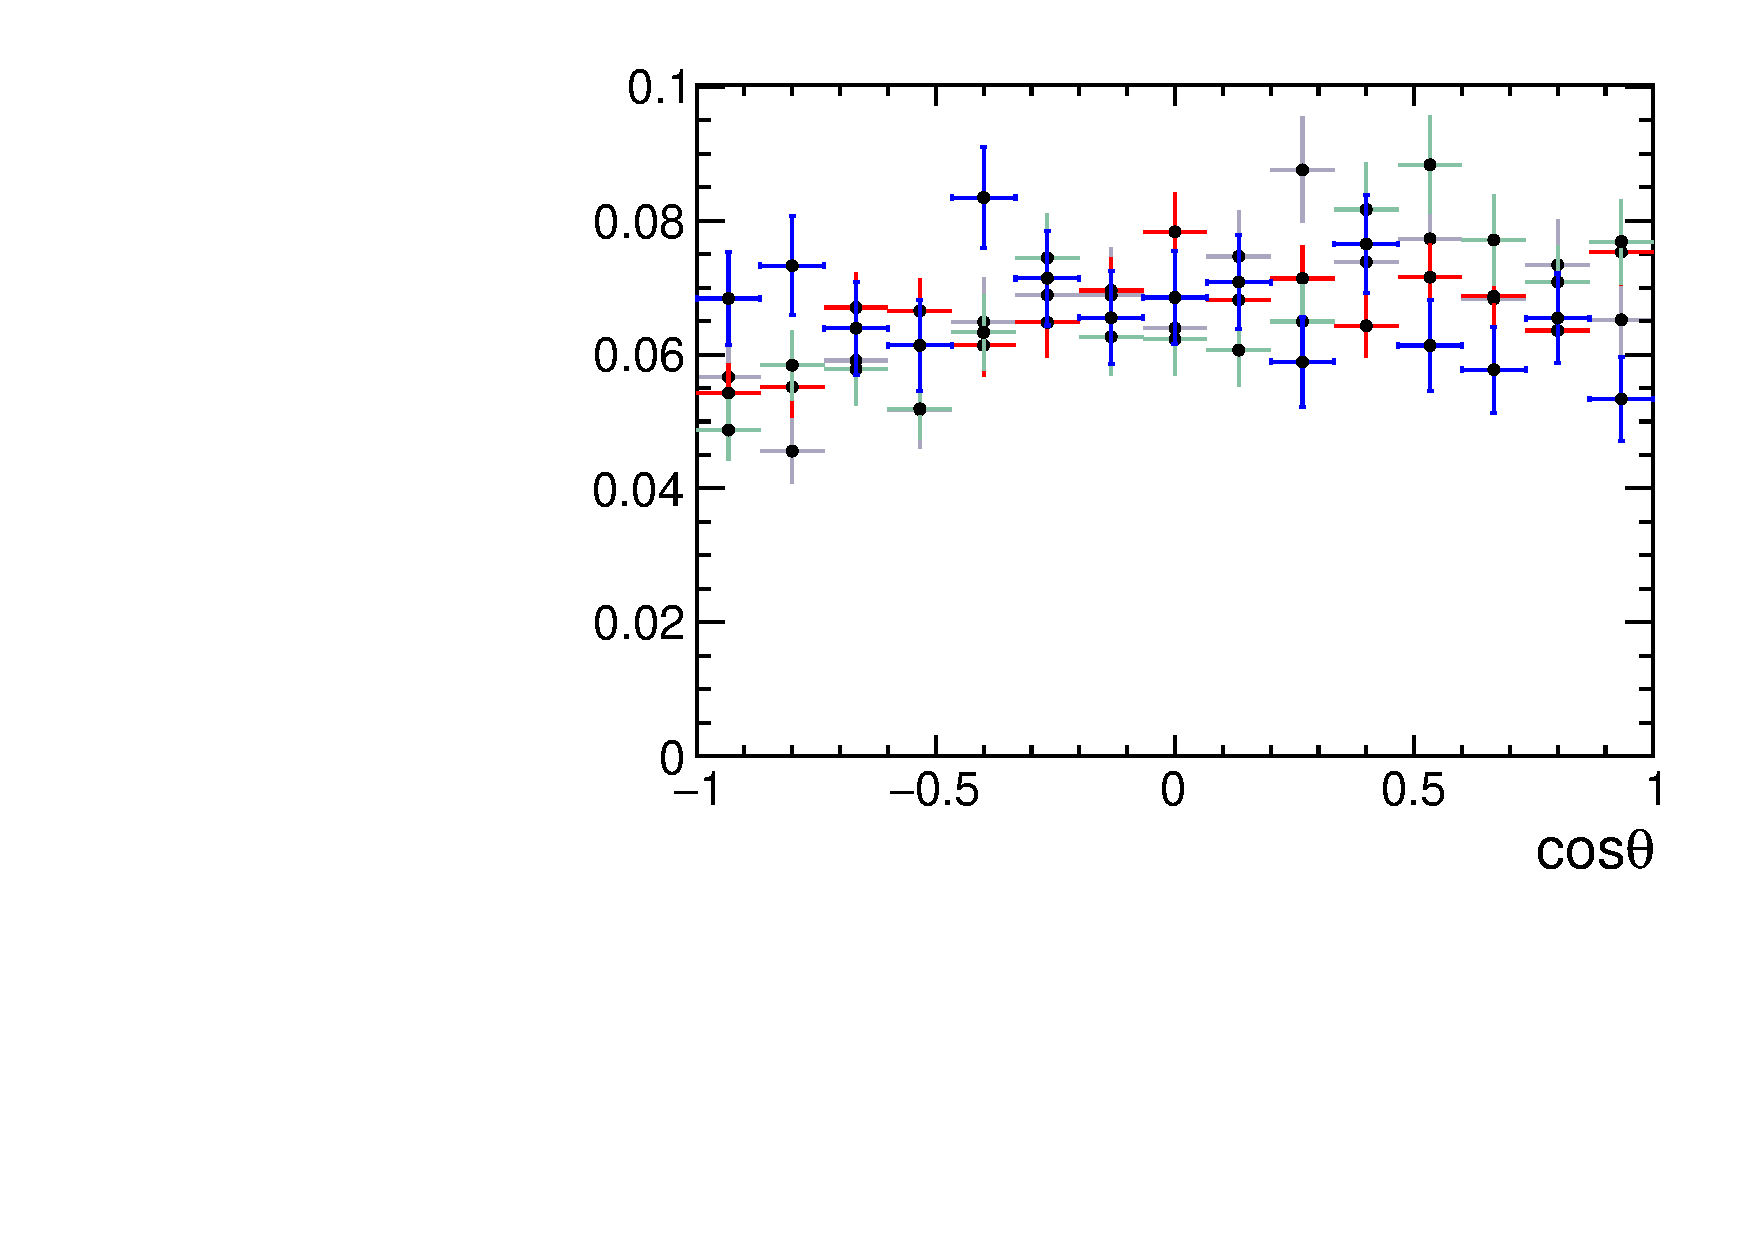
\includegraphics[width=0.4\textwidth]{Figures/05_open_charm/04_tune/poli/kkpi_poli/cosTheta.pdf}%
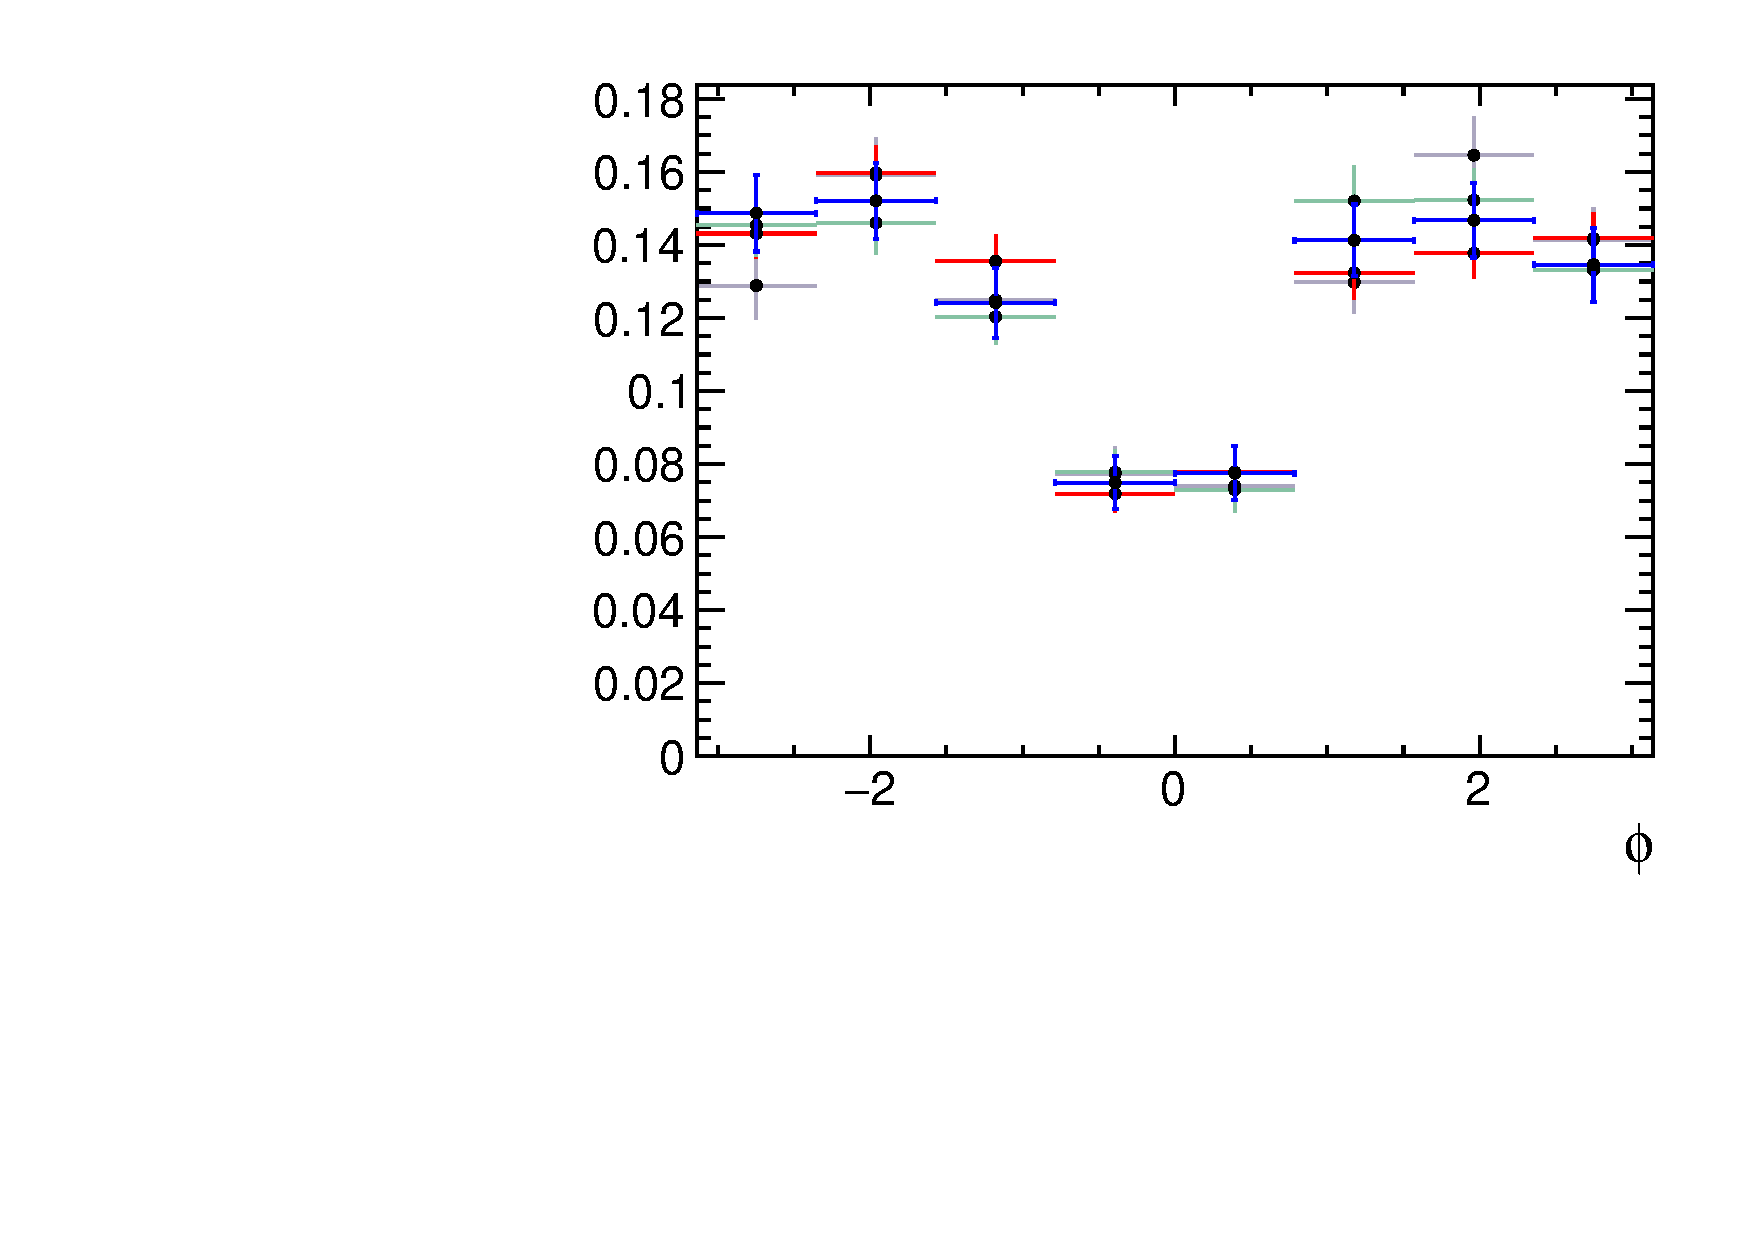
\includegraphics[width=0.4\textwidth]{Figures/05_open_charm/04_tune/poli/kkpi_poli/phi.pdf}\\
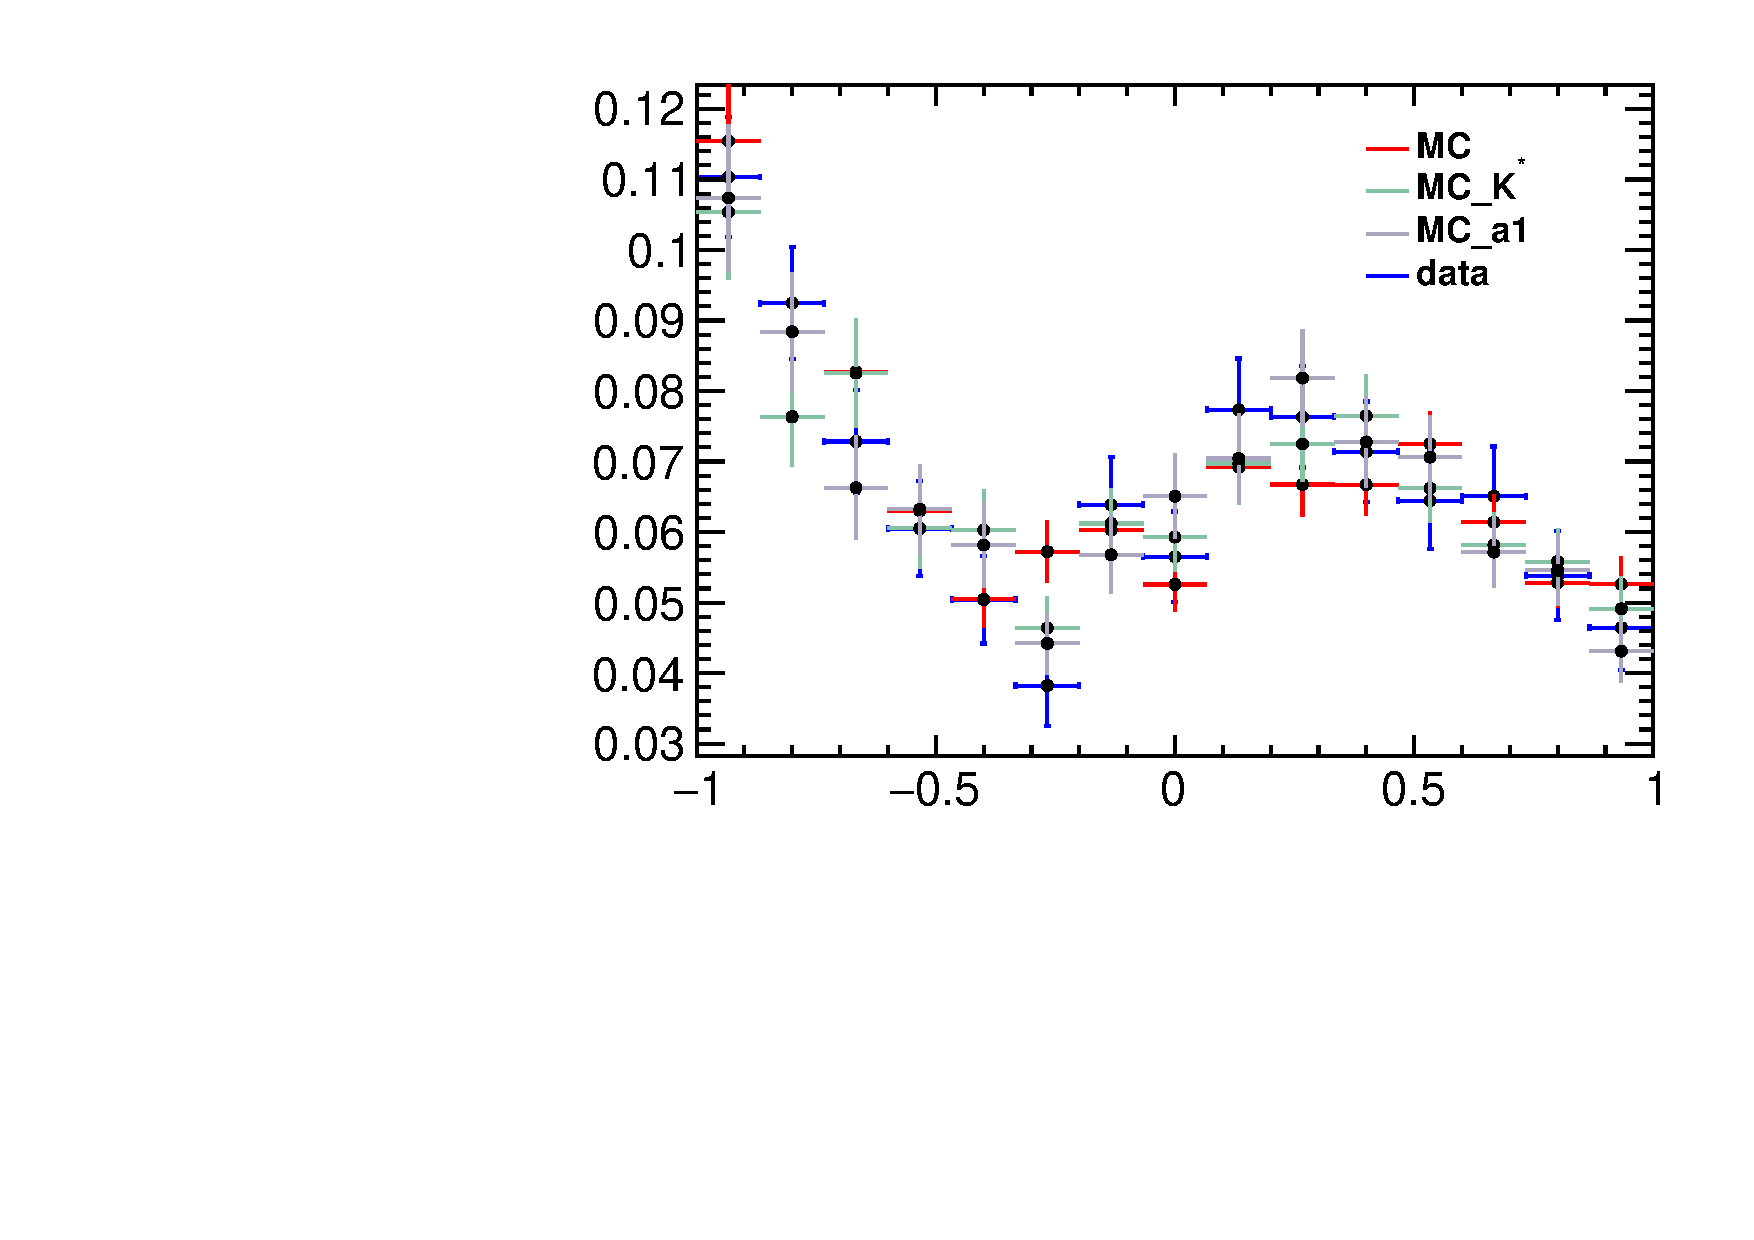
\includegraphics[width=0.4\textwidth]{Figures/05_open_charm/04_tune/poli/kkpi_poli/cosTheta_pk.pdf}%
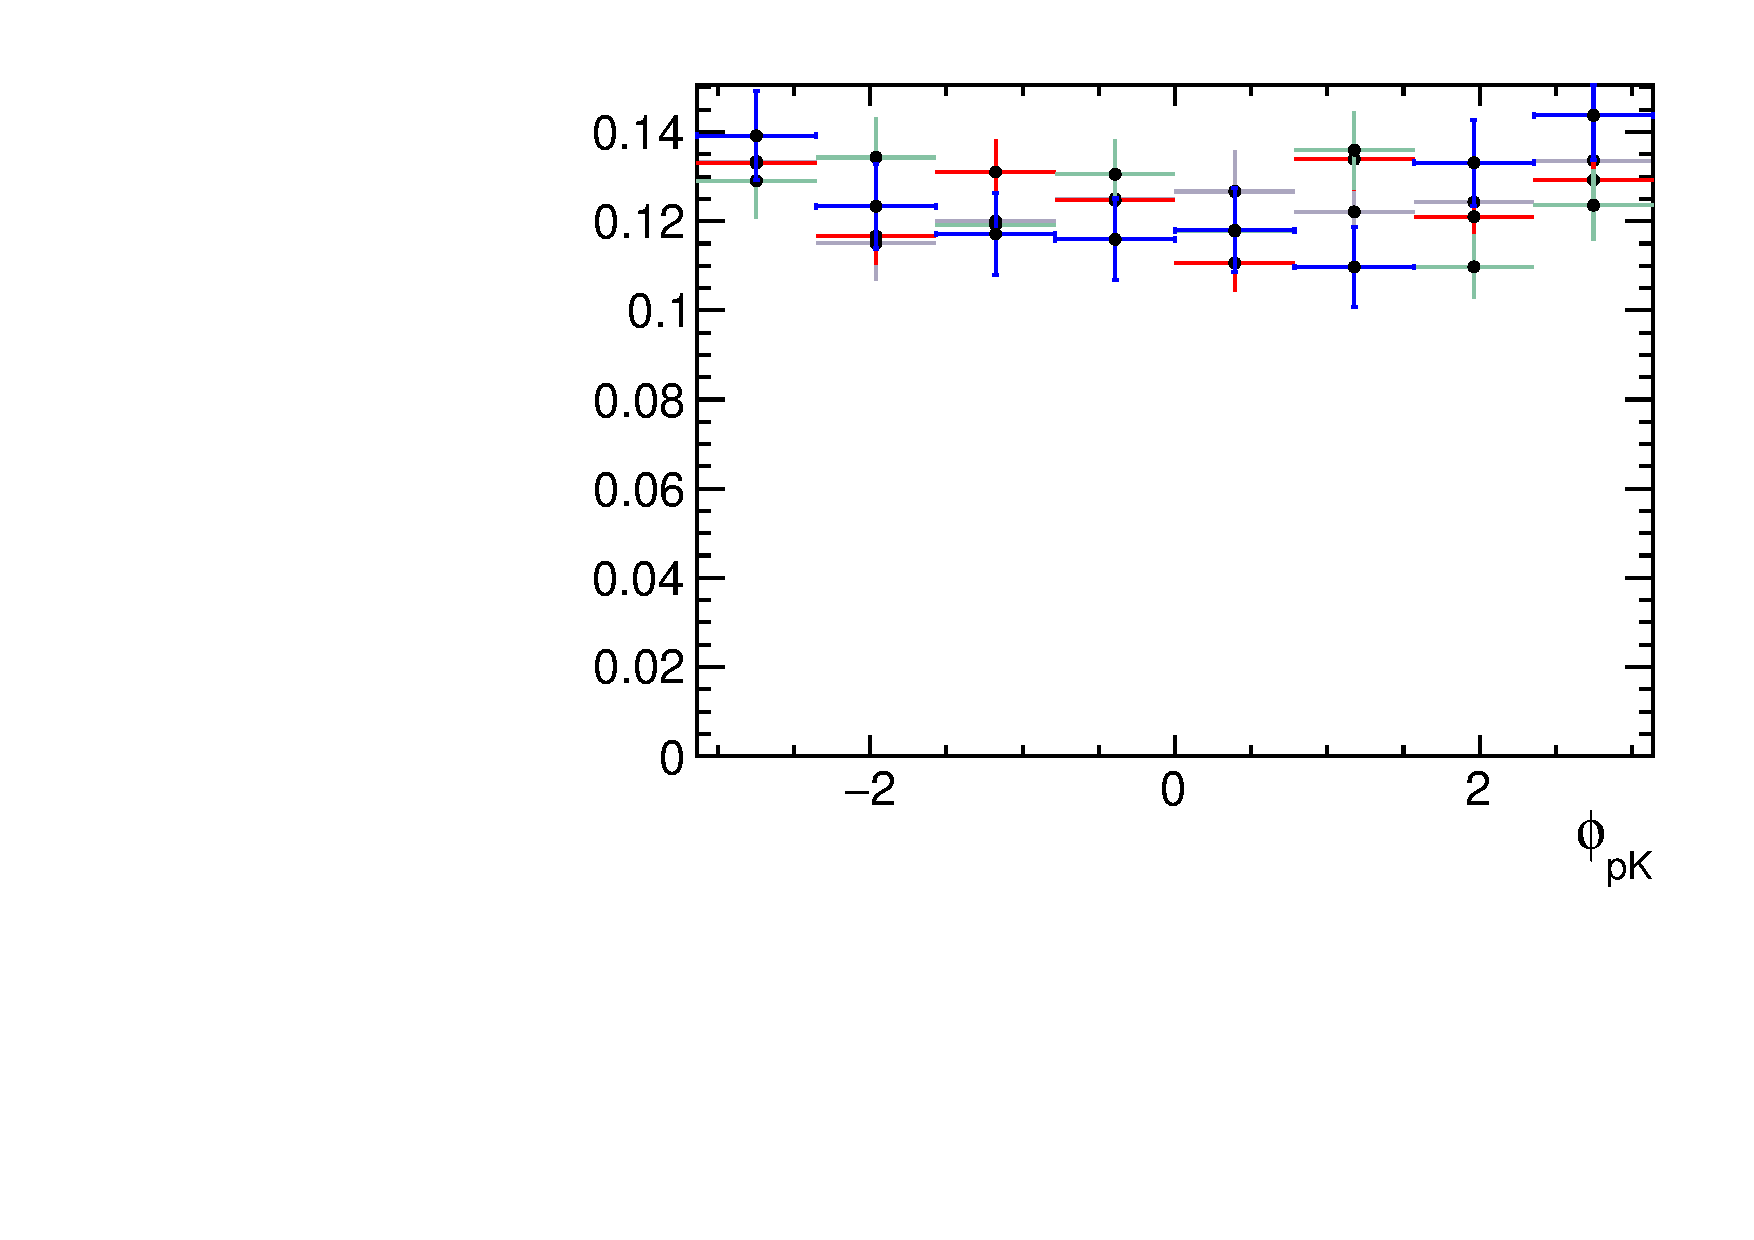
\includegraphics[width=0.4\textwidth]{Figures/05_open_charm/04_tune/poli/kkpi_poli/phi_pk.pdf}\\
	\caption{ The distribution of polarization angle in signal channel}
\label{Fig.poli_kkpi}
\end{figure}


\subsection{Resonances in \LbLckkpi}
\label{sec:resonanceweight}

\begin{figure}[bth]
\centering
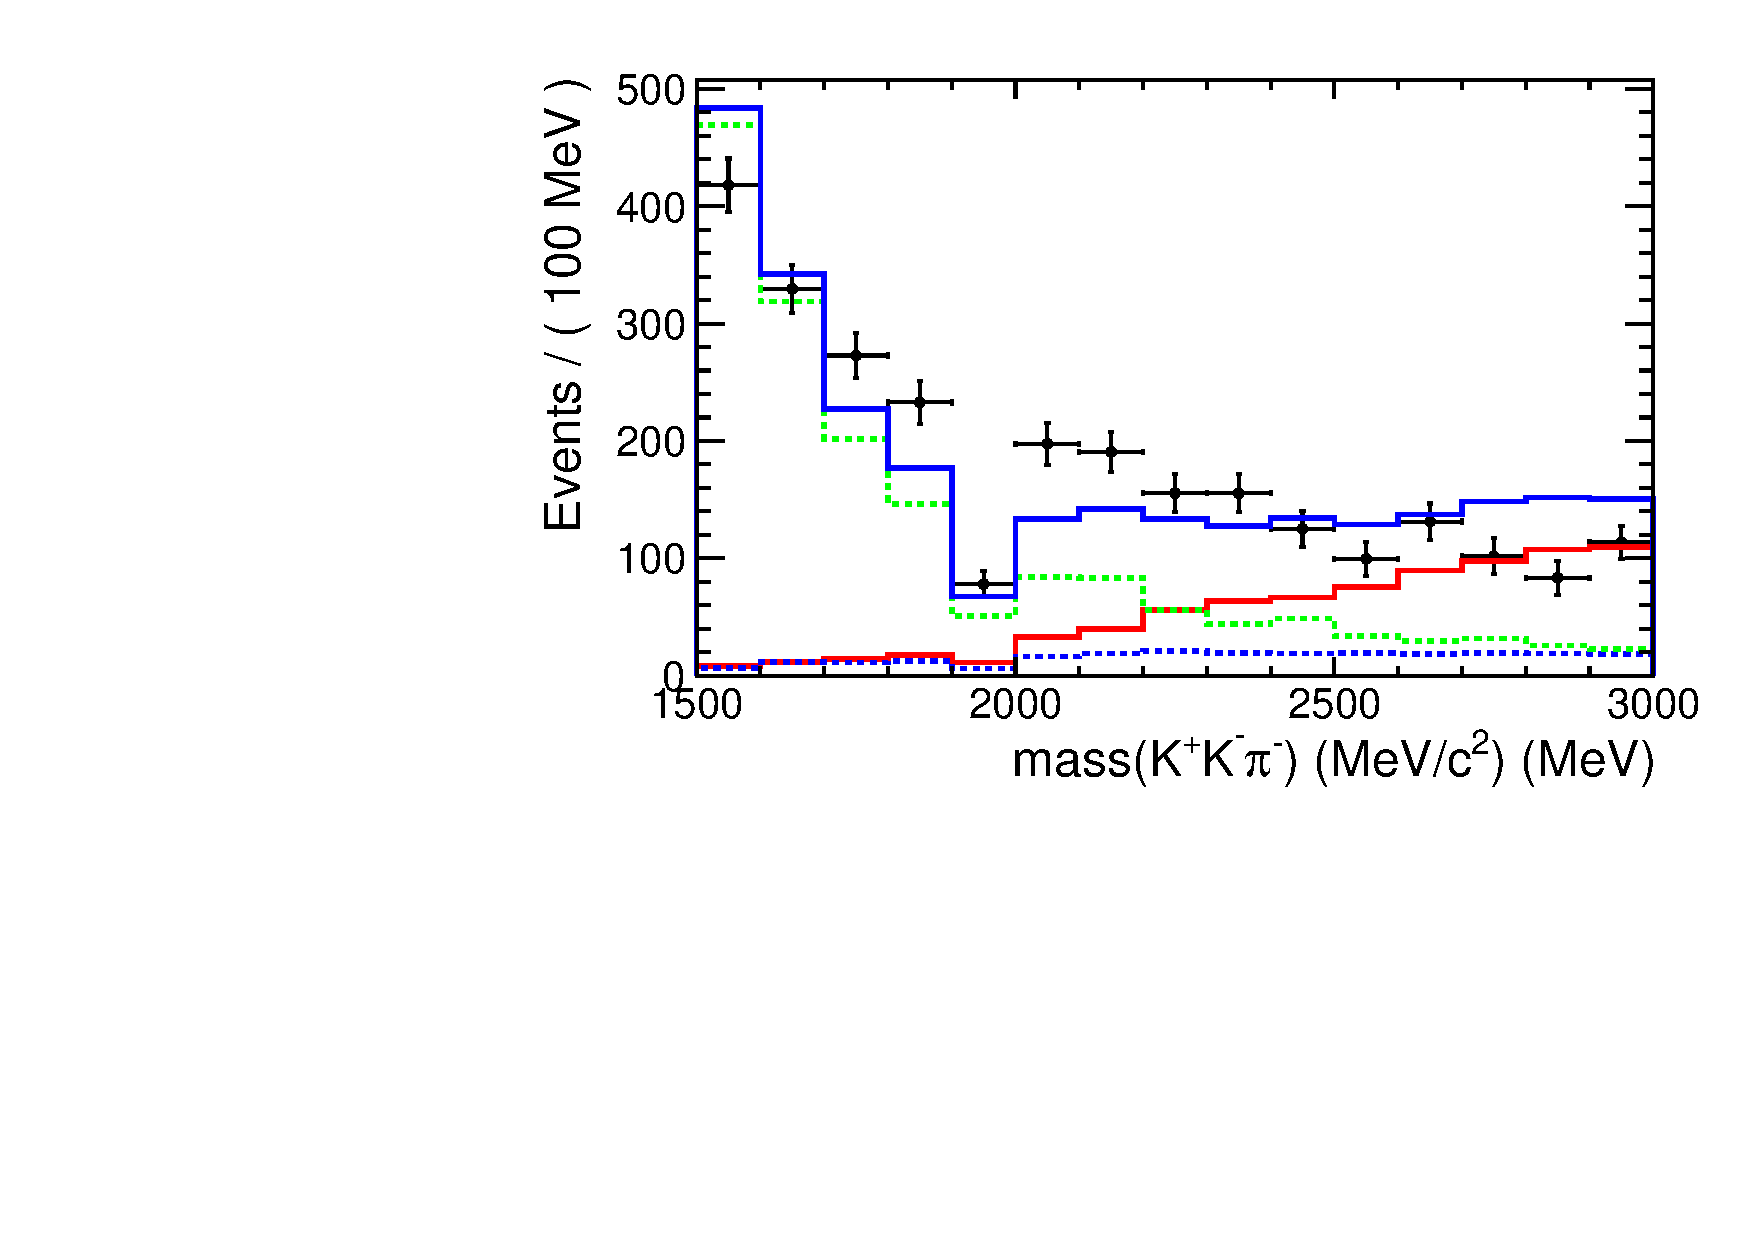
\includegraphics[width=0.4\textwidth]{Figures/05_open_charm/04_tune/component/LbKpKmPi.pdf}%
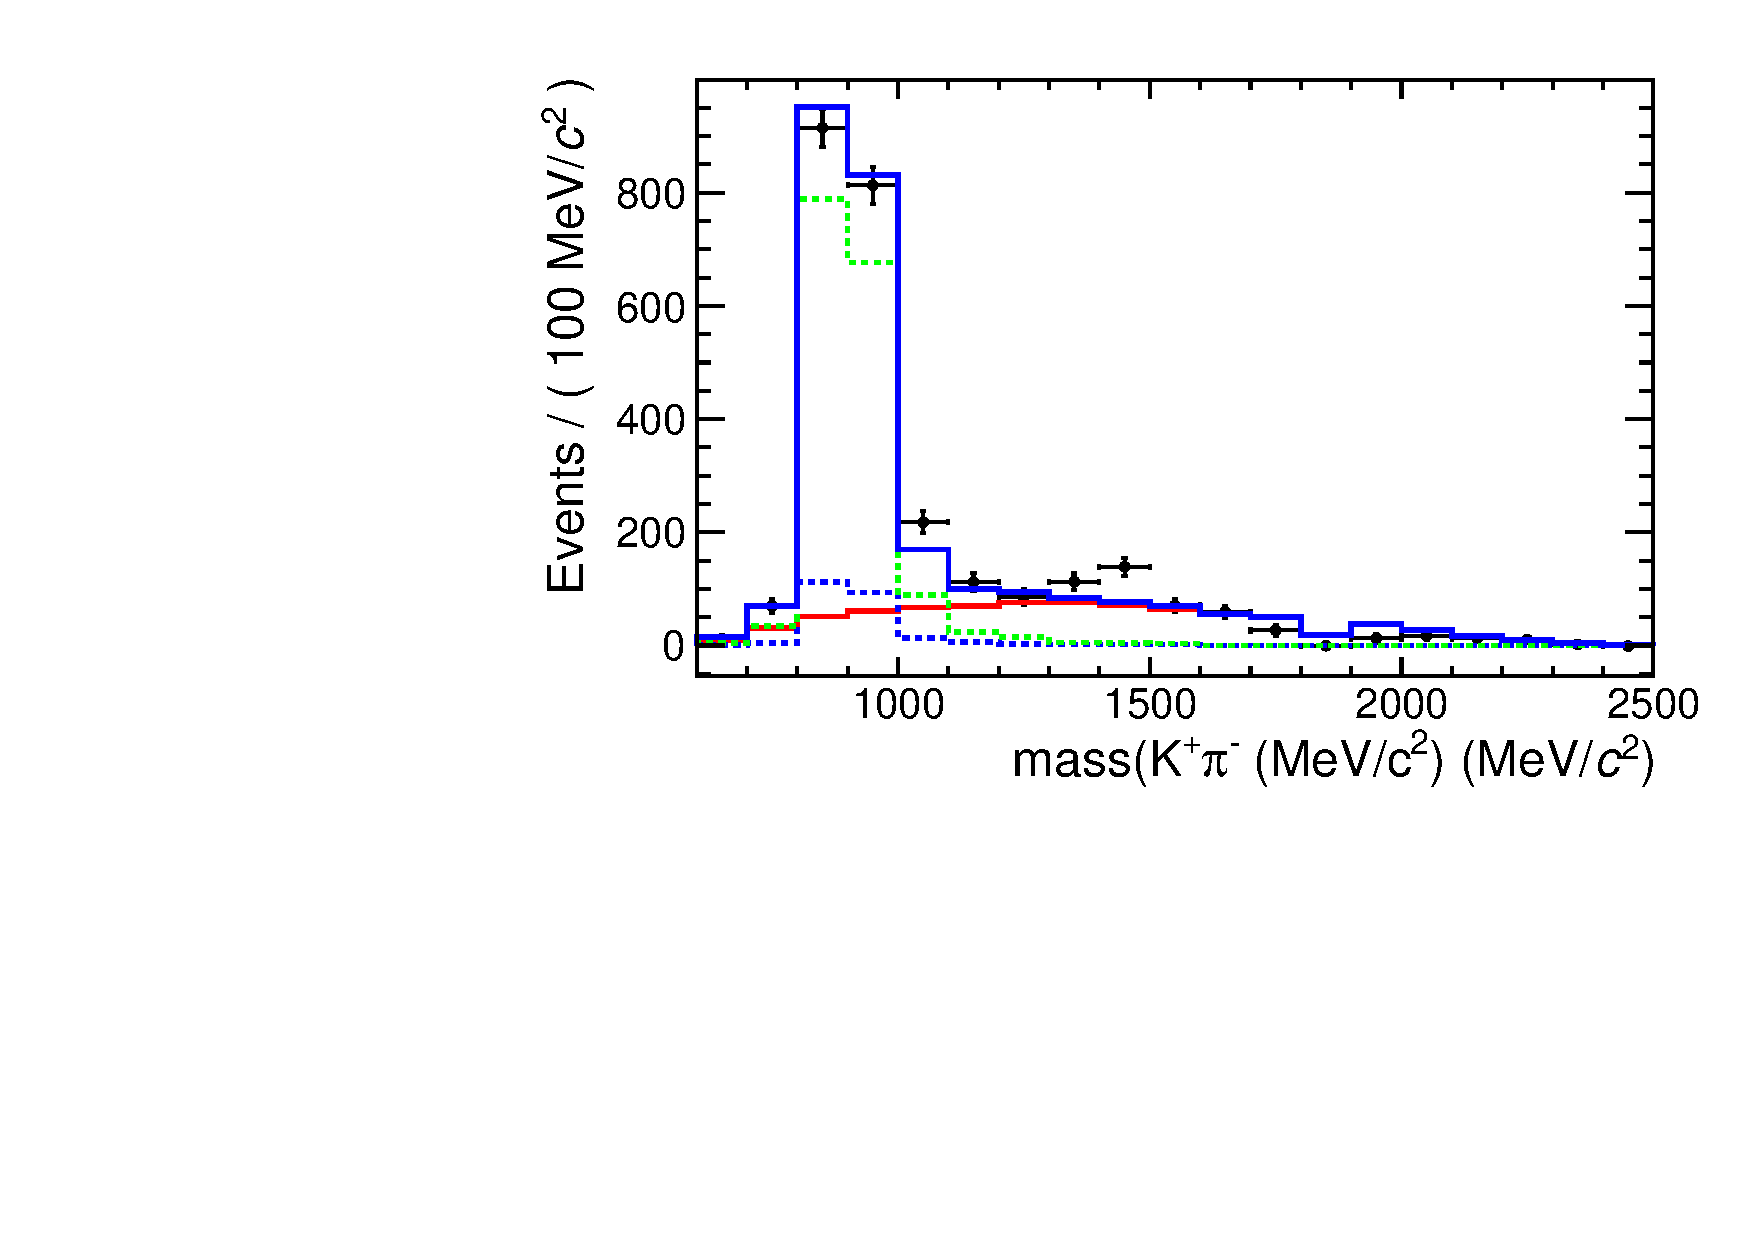
\includegraphics[width=0.4\textwidth]{Figures/05_open_charm/04_tune/component/LbKpPi.pdf}%
\caption{The projection from two dimentions fit, 
the black points are data, 
red line is PHSP sample, 
blue dash line is MC sample with $K^{*}$, 
green dash line is MC sample with $a1$ and blue line is full fit result.}
\label{Fig.Projection}
\end{figure}  

The description of the intermediate states in the signal \Lb decays in simulated events can be different from the real situation, 
many resonances are found in the \LbLckkpi from the data sample while PHSP model is used in the MC sample. 
To estimate the compoments of data sample, 
we fit it using three MC samples -- PHSP $K^+K^-\pi^-$ sample, 
with $K^{*}(892)^0K^-$, and with $a_1(1260)^-\to K^{*}(892)^0K^-$ resonance.  

Comparing the invariant mass distribution of two body combination or three body combination, 
we find the invariant mass of $K^+\pi^-$ and $K^+K^-\pi^-$ have large differences. 
The three MC samples with floating yields are used to fit the background subtracted data distributions 
of two dimensional invariant masses of $K^+\pi^-$ and $K^+K^-\pi^-$, 
the projected distributions are shown in Figure.~\ref{Fig.Projection}. 

The fitting fractions are used to construct a blended MC sample to better describe data.
The fitting results are listed in Table~\ref{tab:MassFit_component}.   

\begin{table}[!btp]
\centering
\caption{Fit result of \LbLckkpi using MC smaples.}
\vspace{0.2cm}
\label{tab:MassFit_component}
\begin{tabular}{c c }\hline\hline
Parameter         	& Number             \\\hline
$n_{nonresonance}$ & 824.1  $\pm$  36.7 \\
$n_{K^{*}}$        & 275.2  $\pm$  49.2 \\
$n_{a_1(1260)^-}$  & 2059.8 $\pm$  61.4 \\
\hline\hline
\end{tabular}
\end{table}

\begin{figure}[bth]
\centering
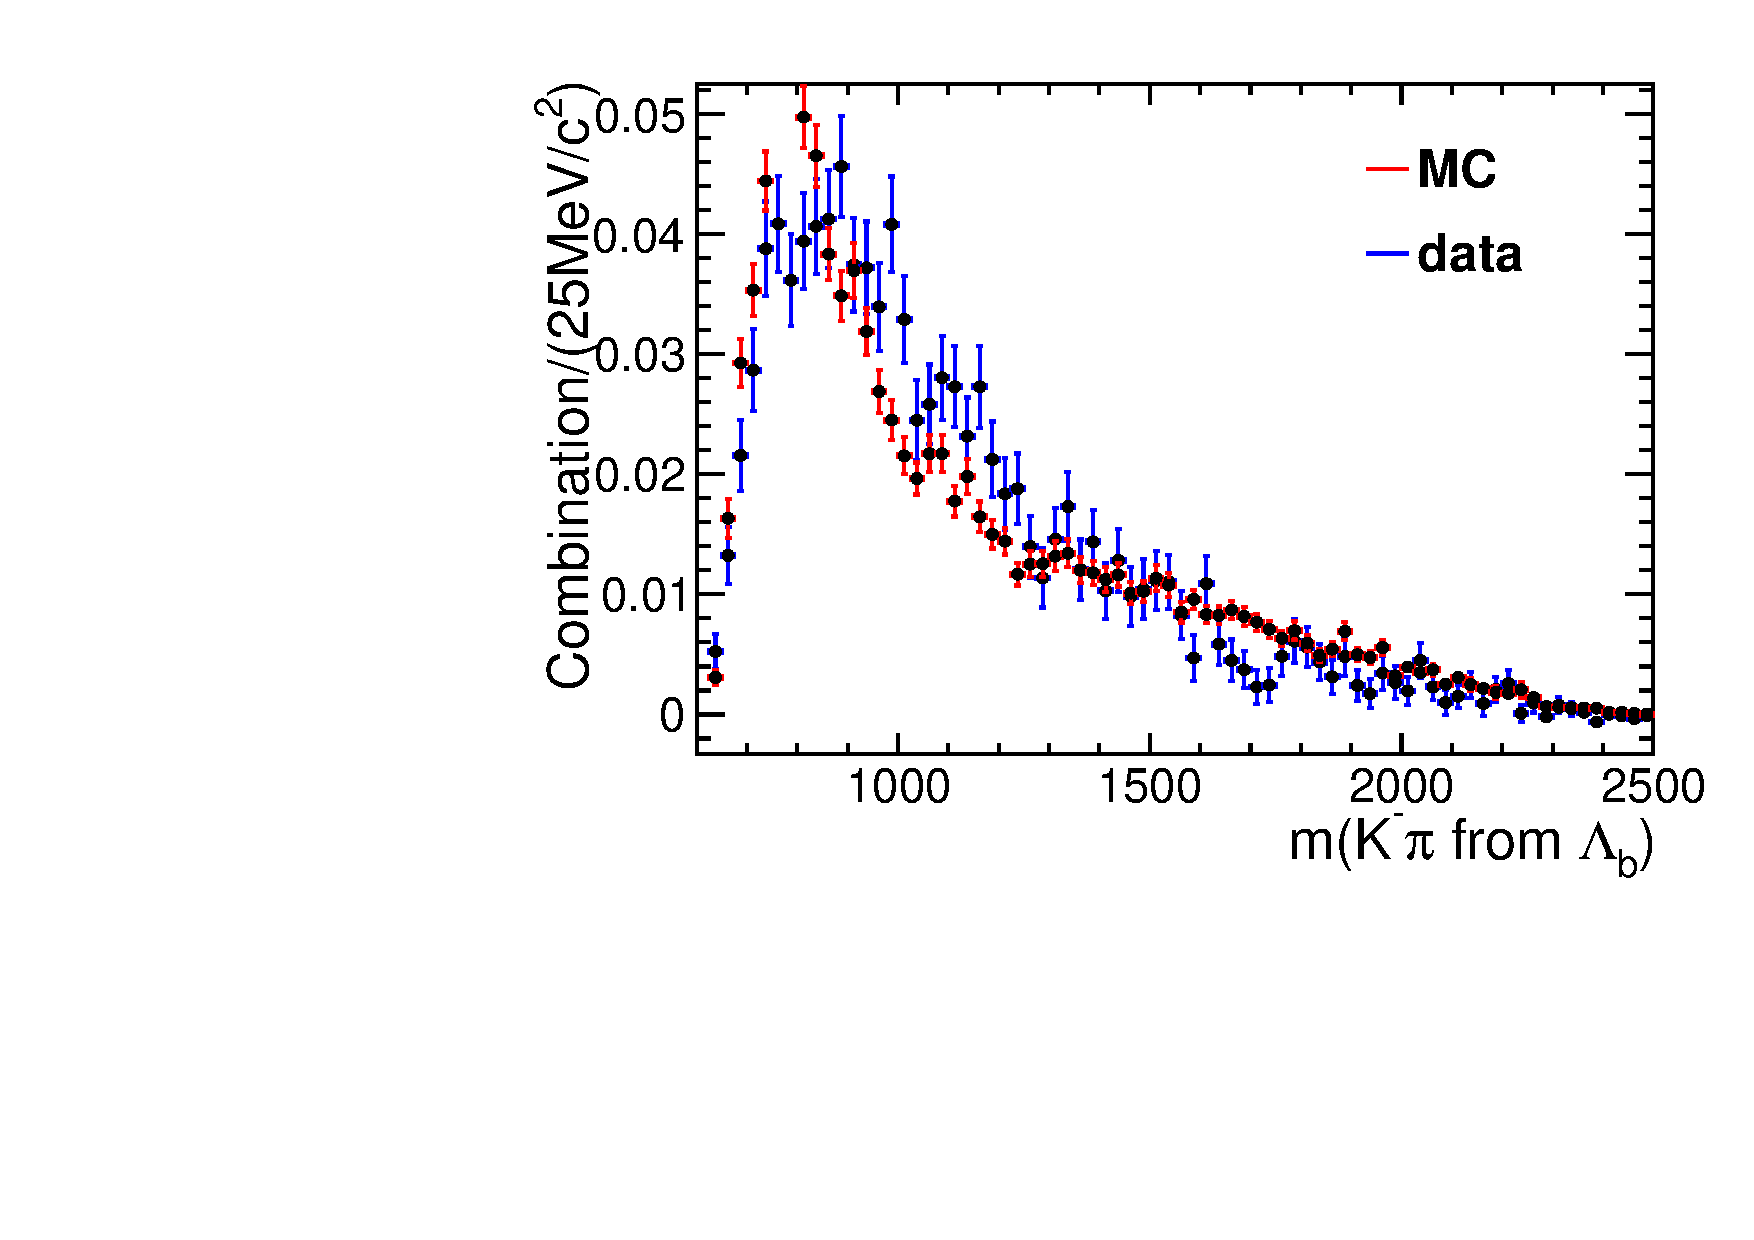
\includegraphics[width=0.4\textwidth]{Figures/05_open_charm/04_tune/new_for_note/LbKmPi_M.pdf}%
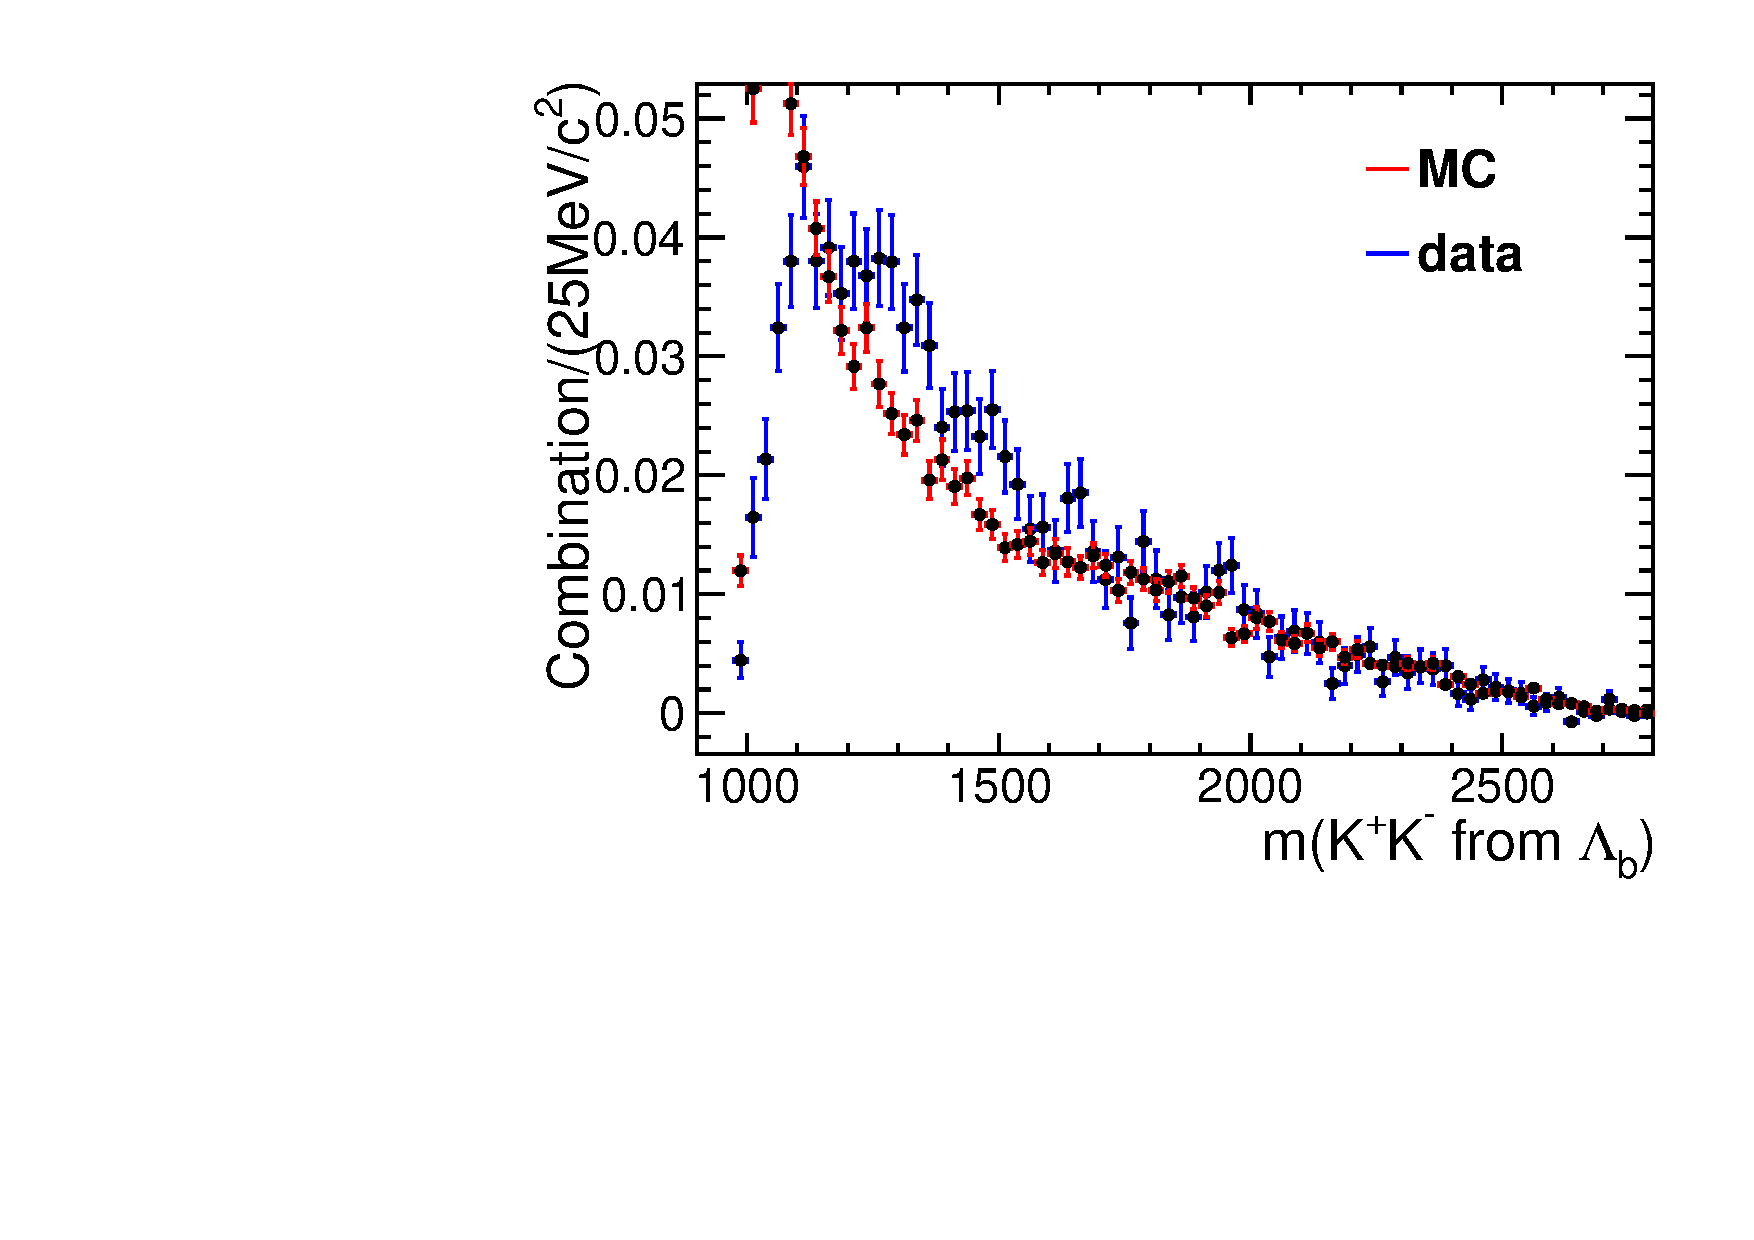
\includegraphics[width=0.4\textwidth]{Figures/05_open_charm/04_tune/new_for_note/LbKpKm_M.pdf}\\%
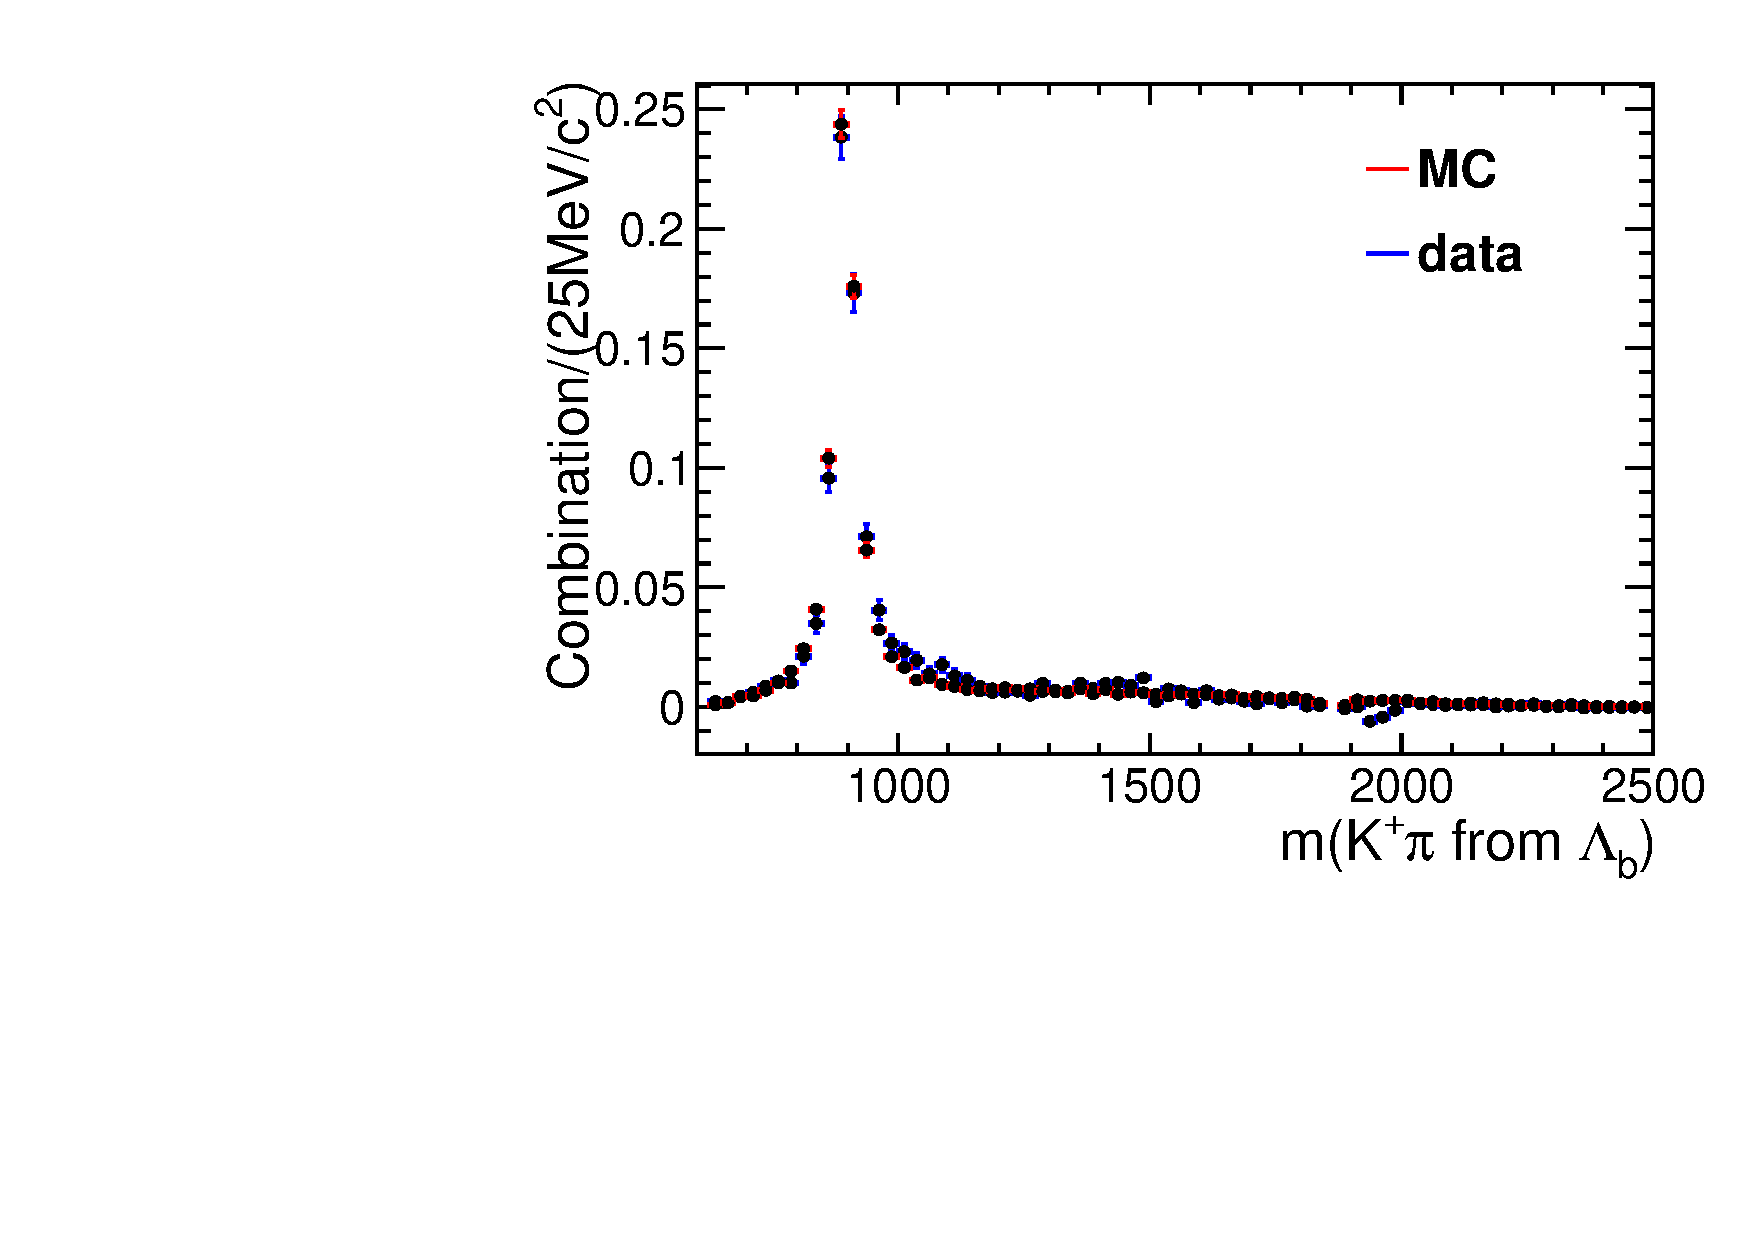
\includegraphics[width=0.4\textwidth]{Figures/05_open_charm/04_tune/new_for_note/LbKpPi_M.pdf}%
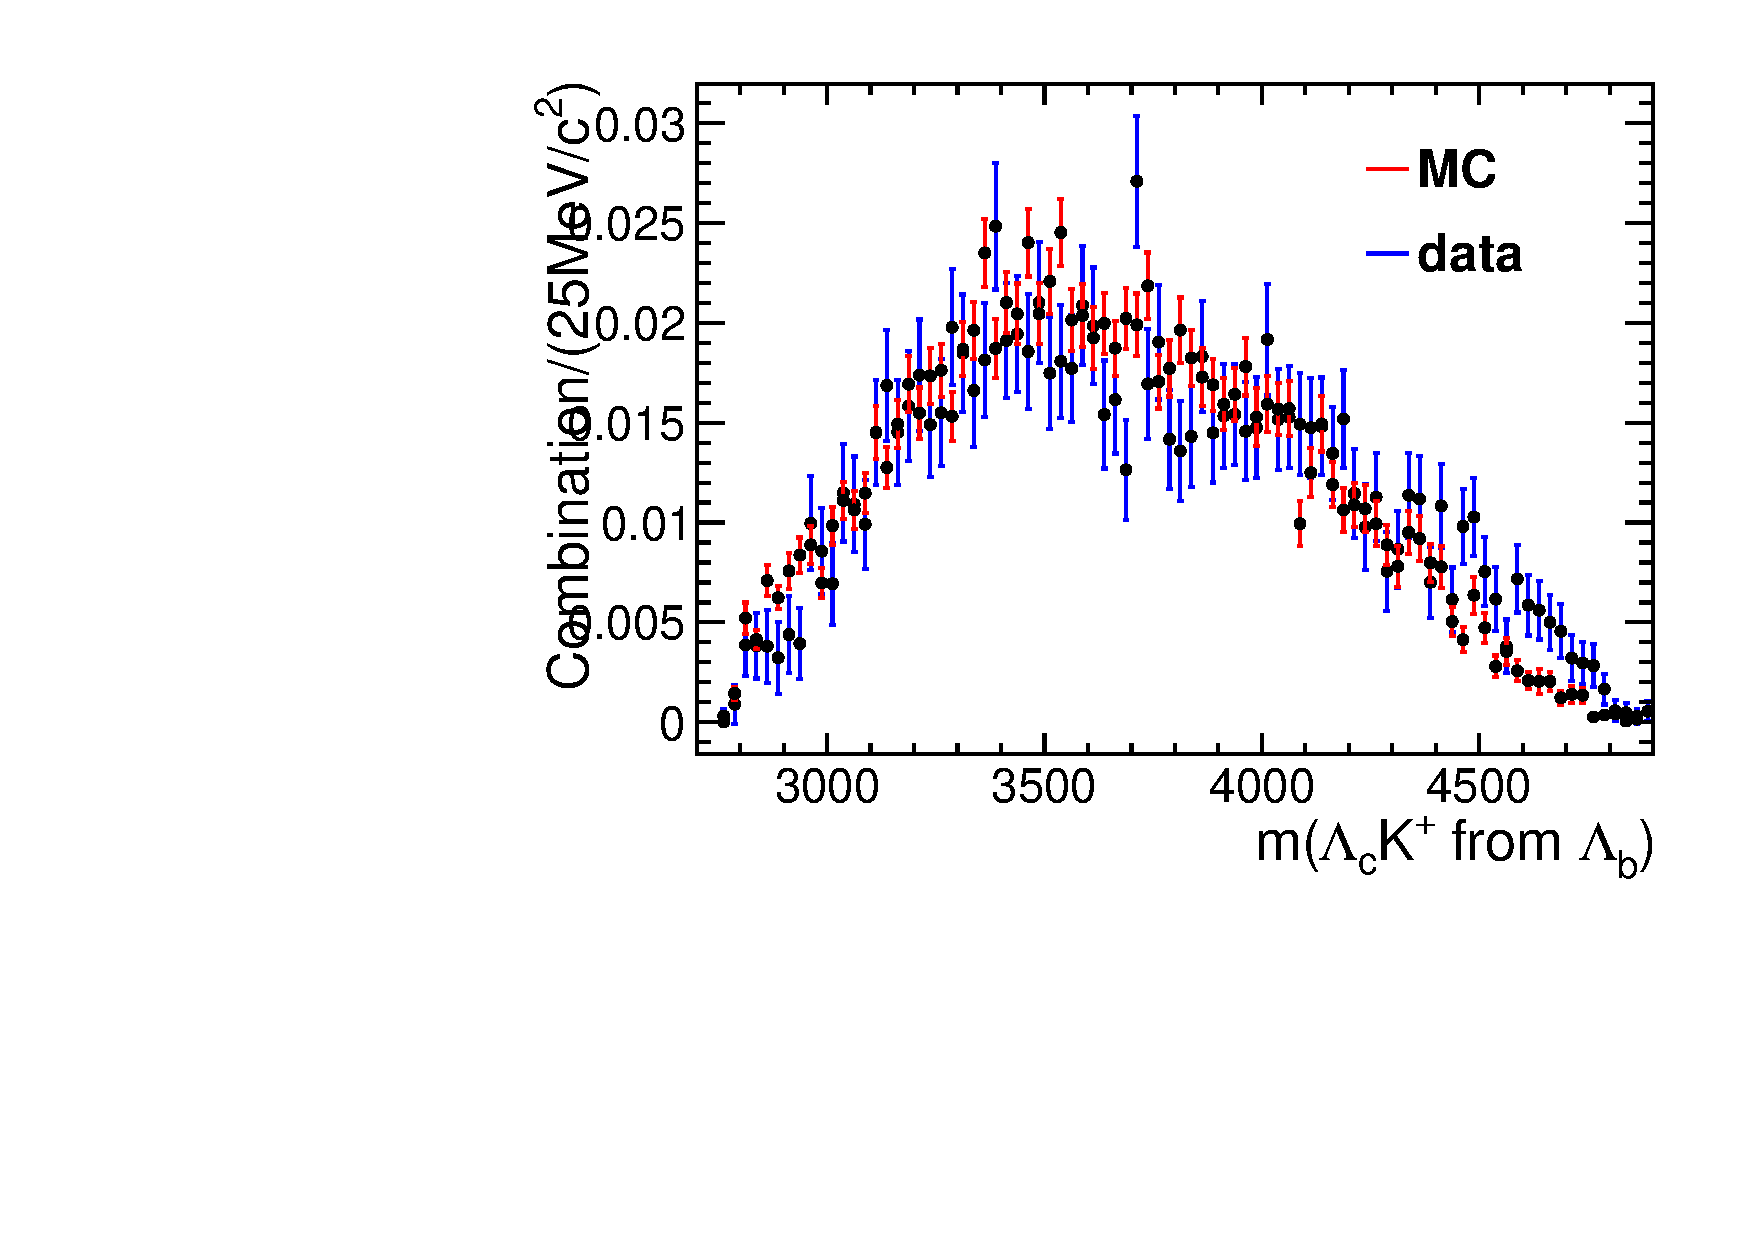
\includegraphics[width=0.4\textwidth]{Figures/05_open_charm/04_tune/new_for_note/LcLbKp_M_con.pdf}\\
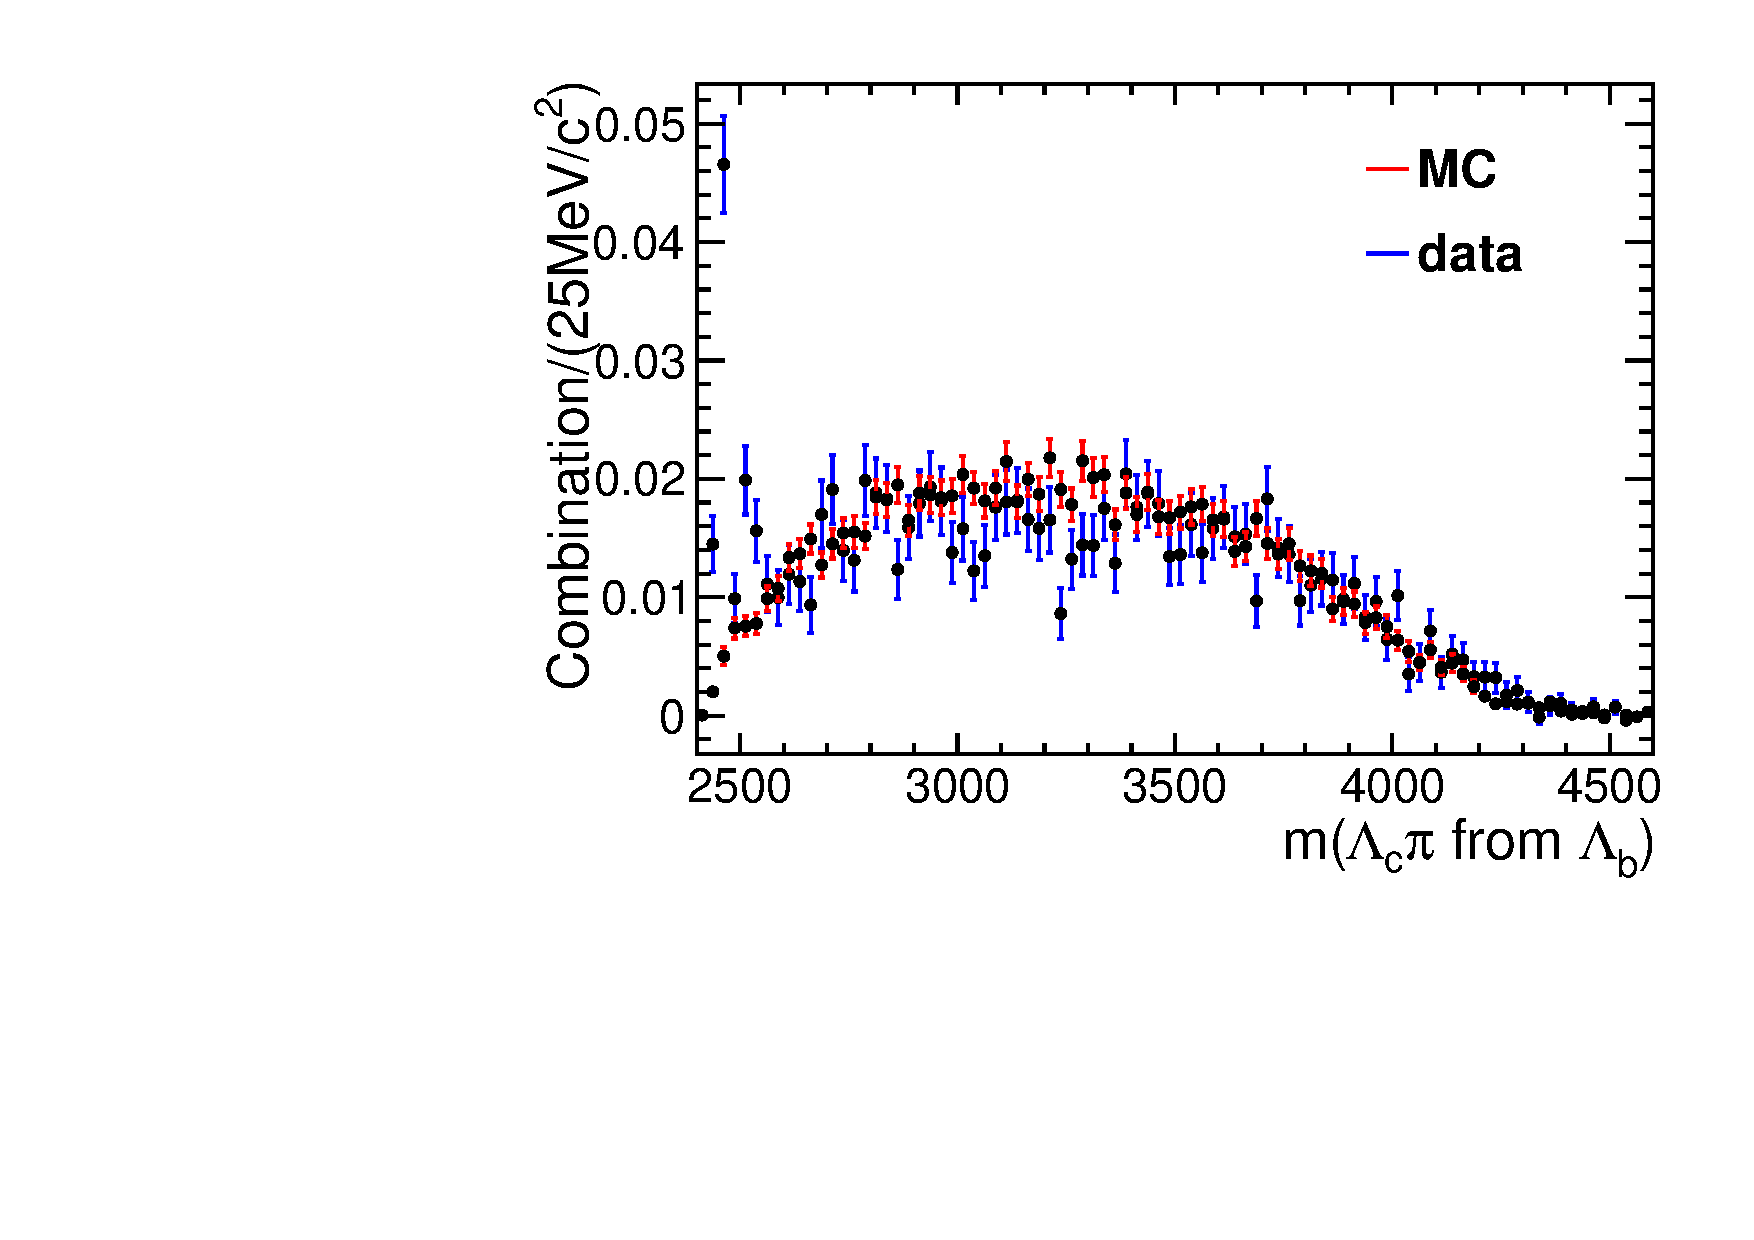
\includegraphics[width=0.4\textwidth]{Figures/05_open_charm/04_tune/new_for_note/LcLbPi_M_con.pdf}%
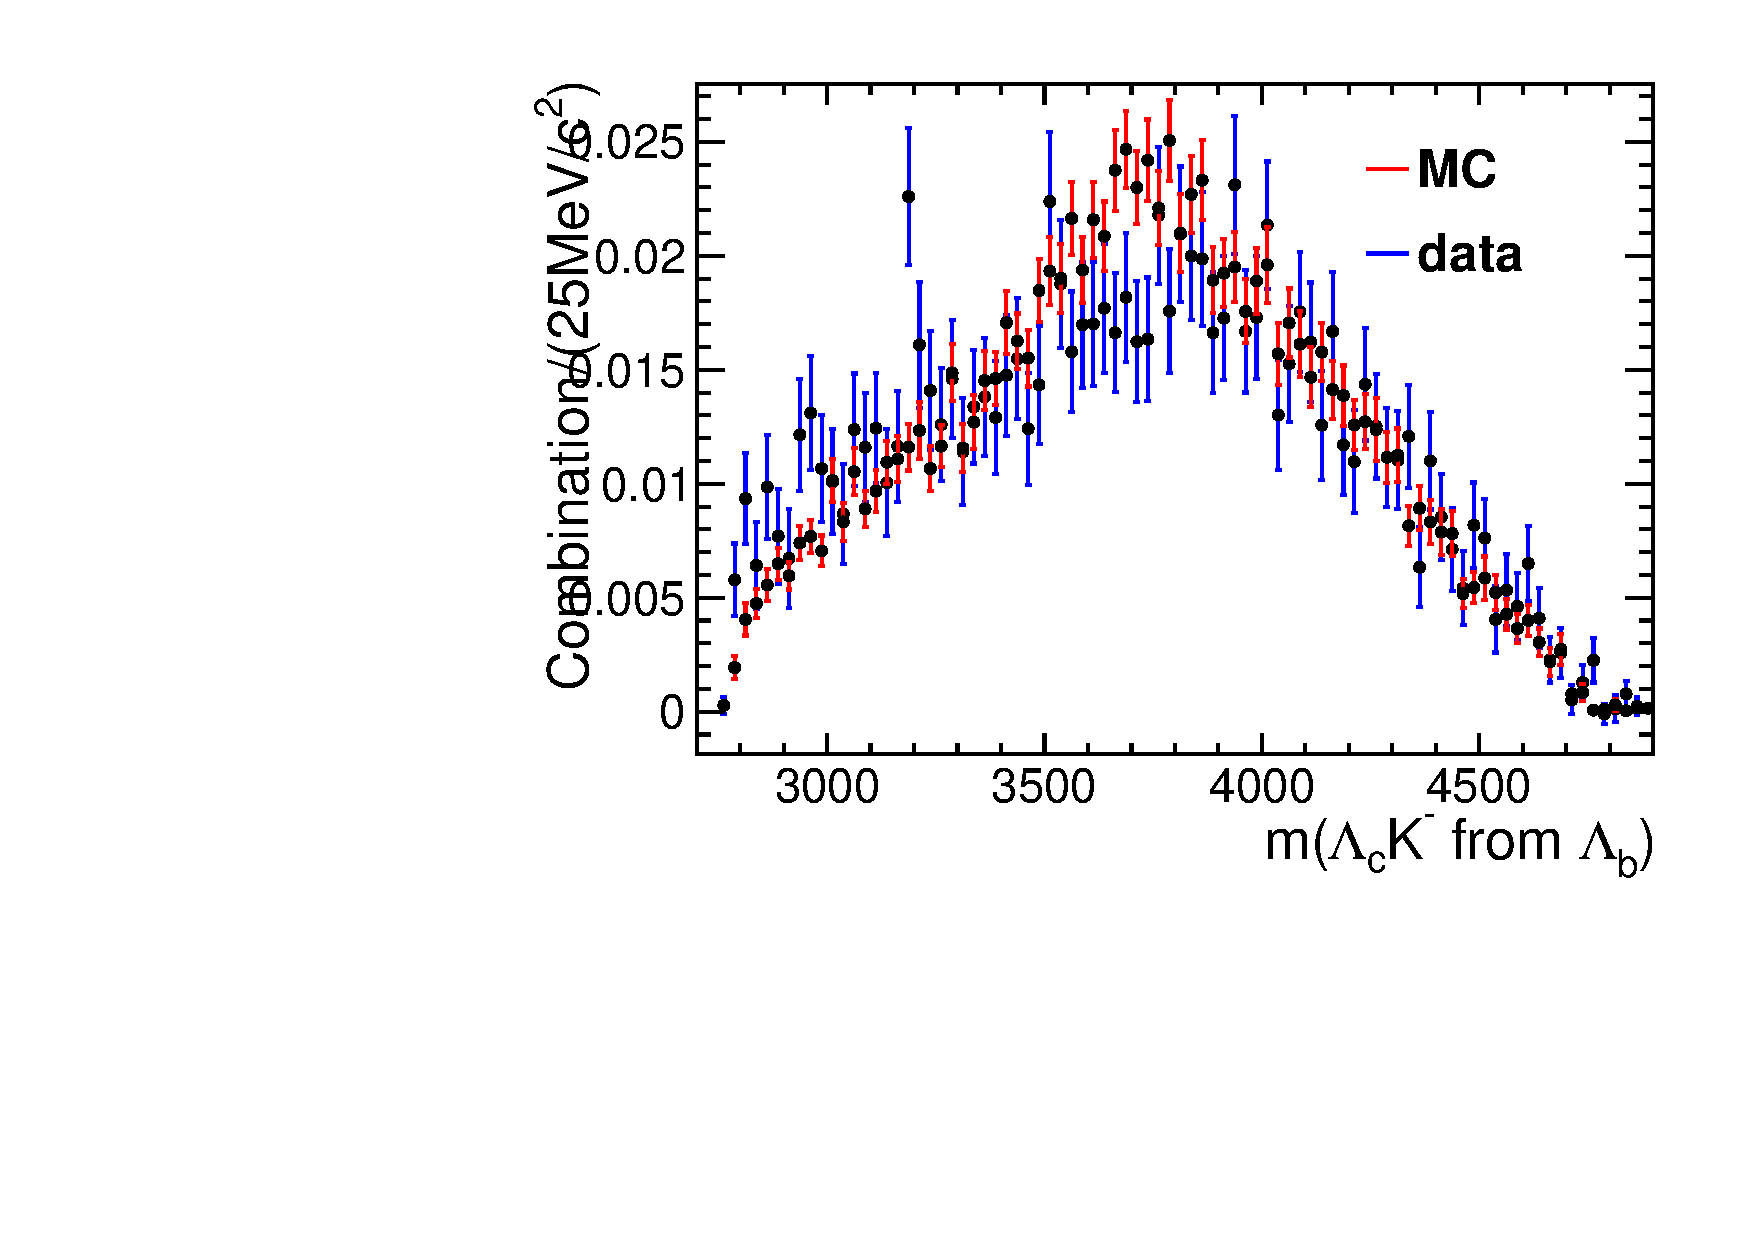
\includegraphics[width=0.4\textwidth]{Figures/05_open_charm/04_tune/new_for_note/LcLbKm_M_con.pdf}\\%
\caption{The invariant mass distribution of  two body combination for \LbLckkpi in the background subtracted data and MC.}
\label{fig.Resonance_2body}
\end{figure}  

\begin{figure}[bth]
\centering
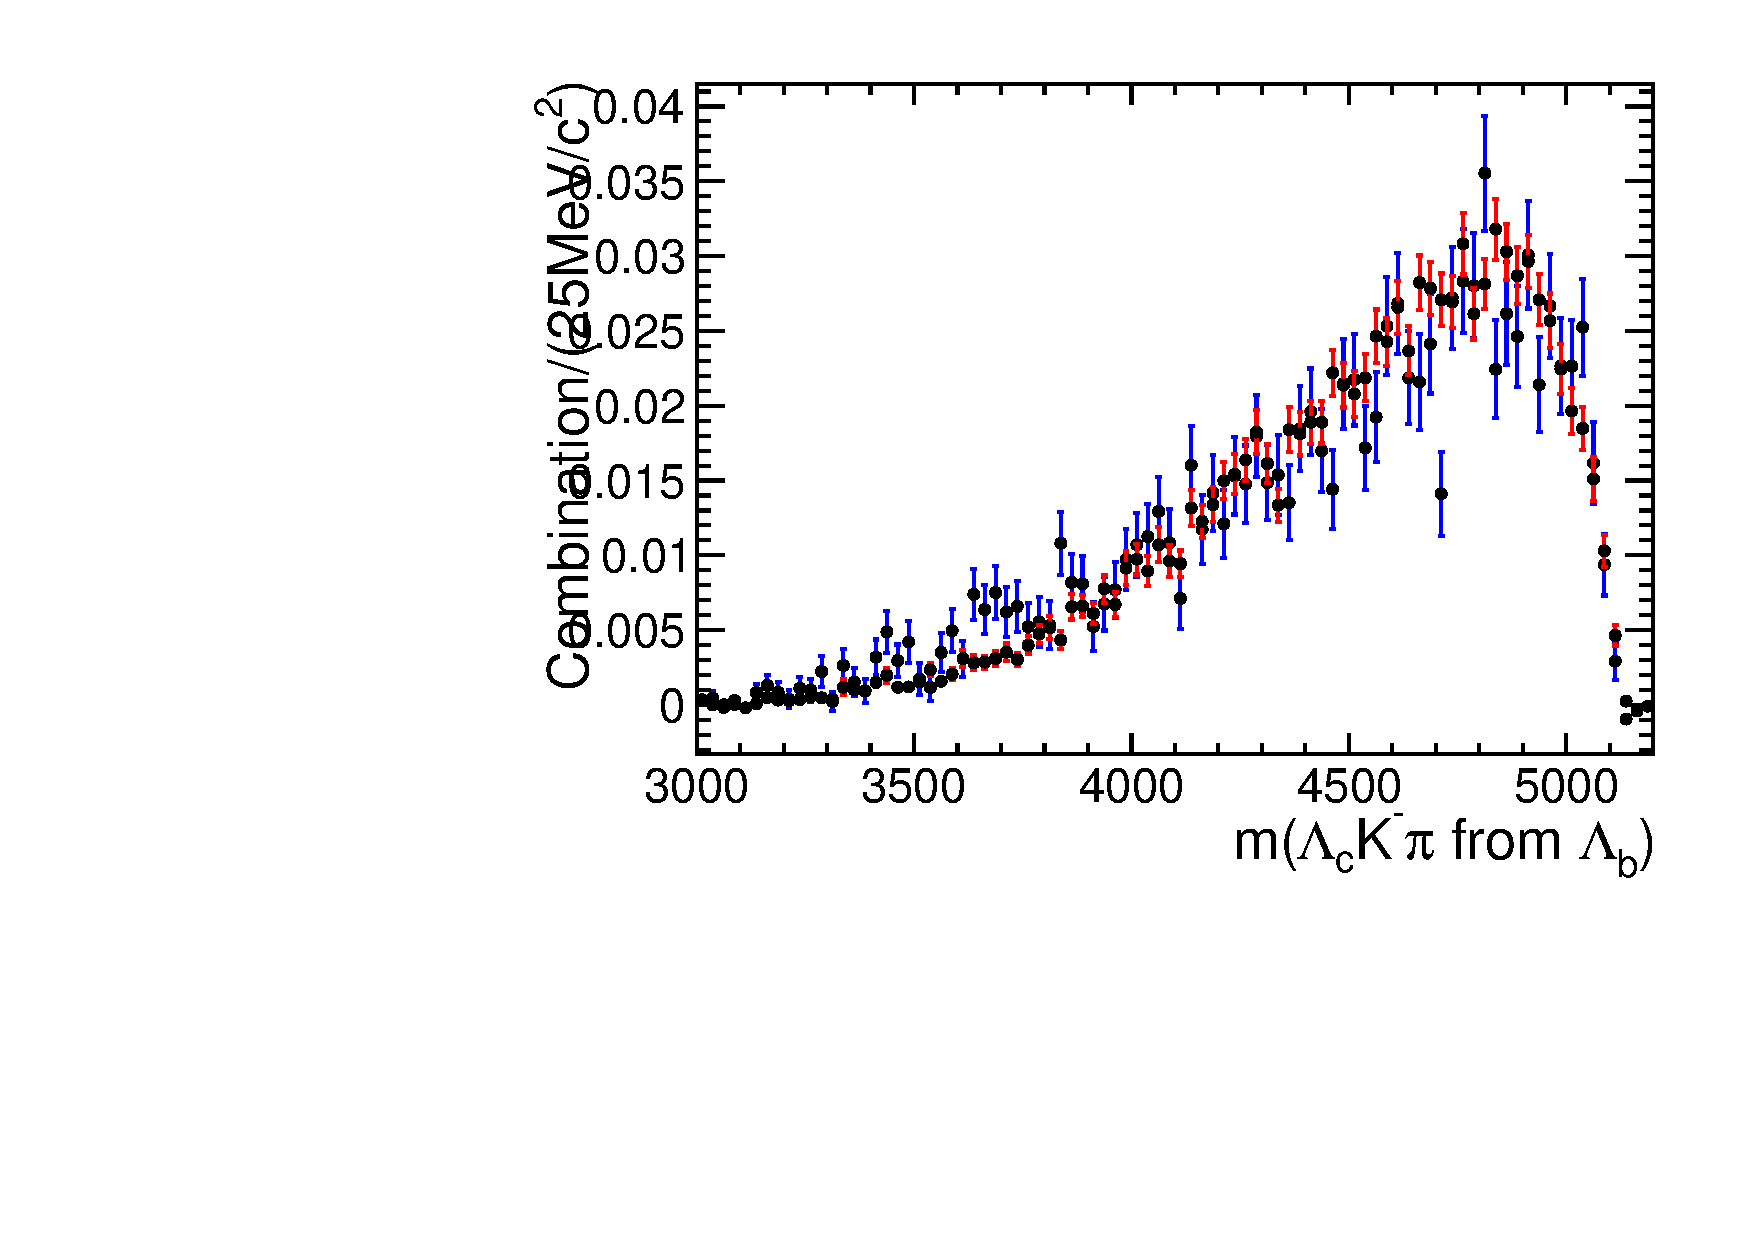
\includegraphics[width=0.4\textwidth]{Figures/05_open_charm/04_tune/new_for_note/LcLbKmPi_M_con.pdf}%
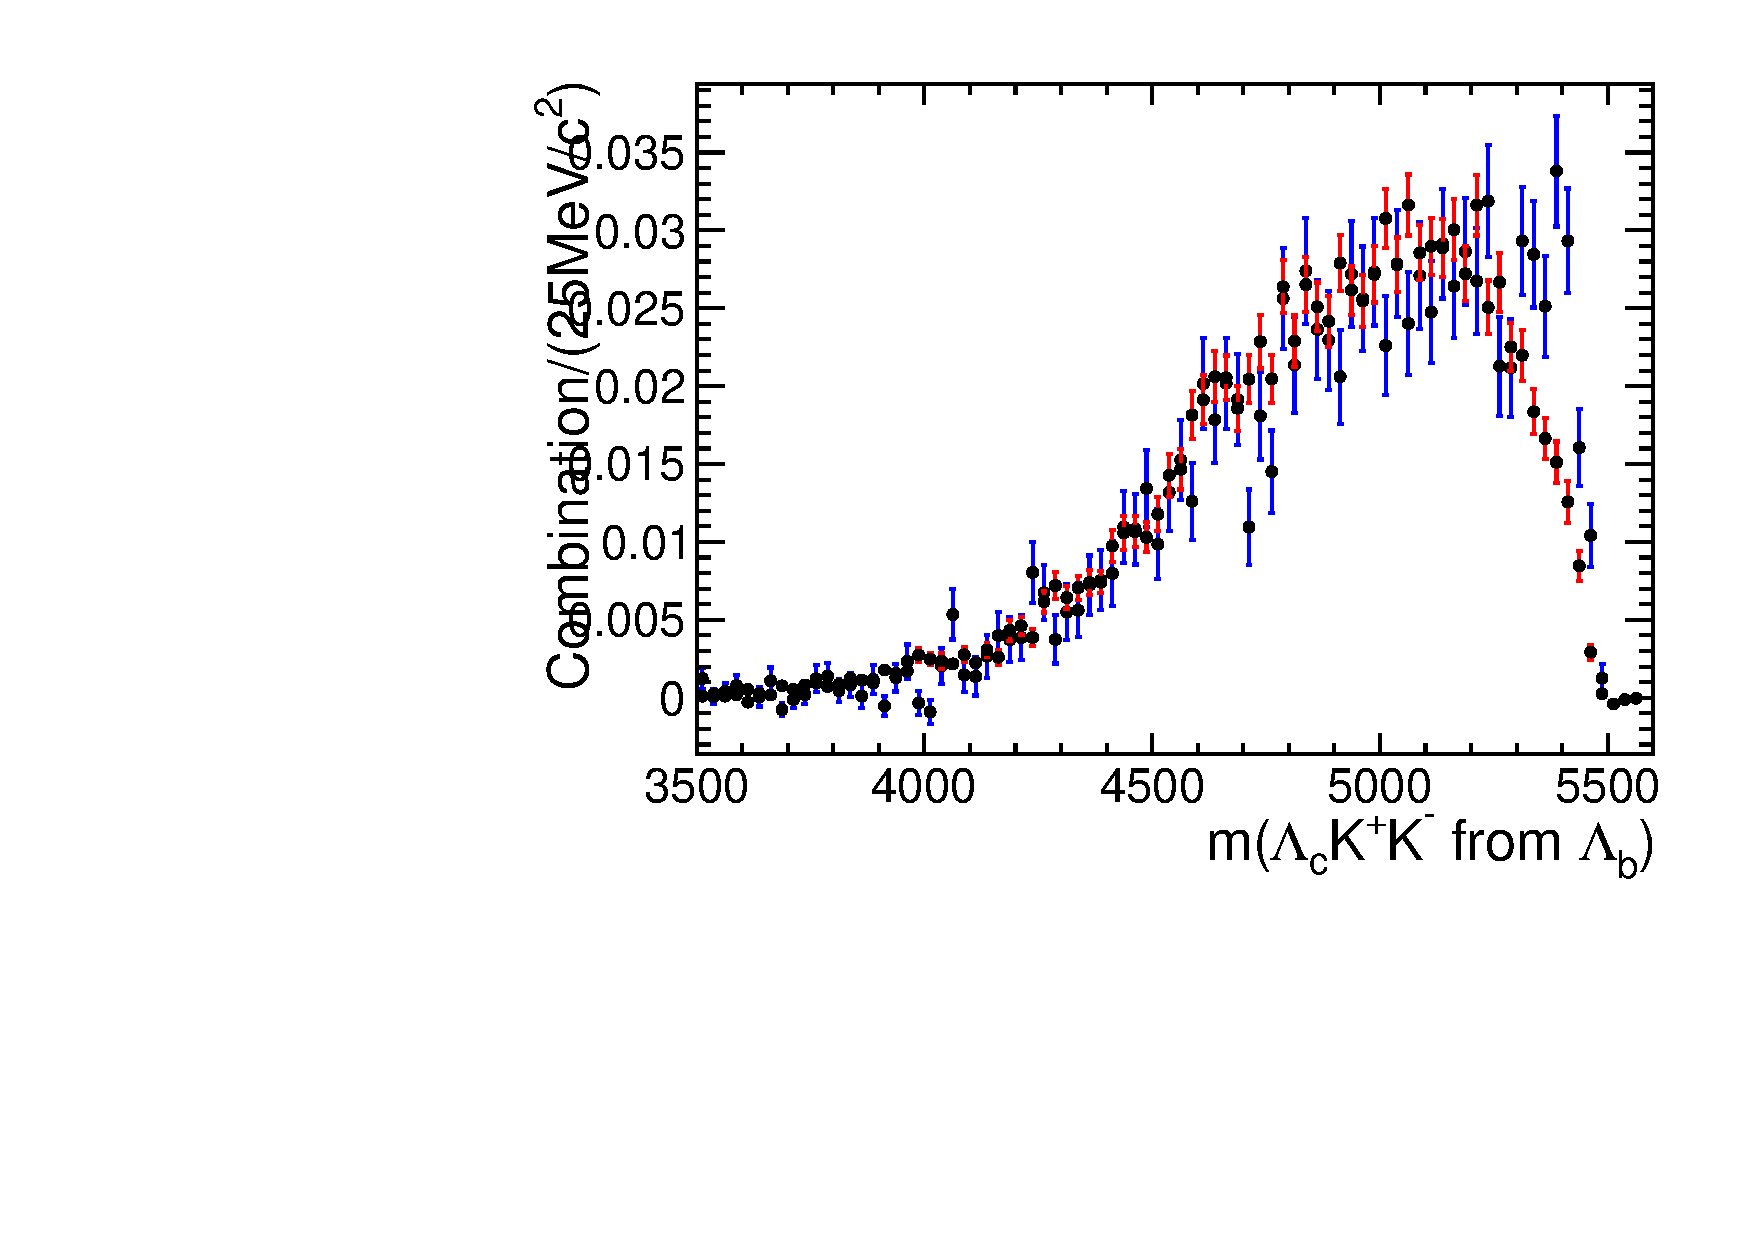
\includegraphics[width=0.4\textwidth]{Figures/05_open_charm/04_tune/new_for_note/LcLbKpKm_M_con.pdf}\\%
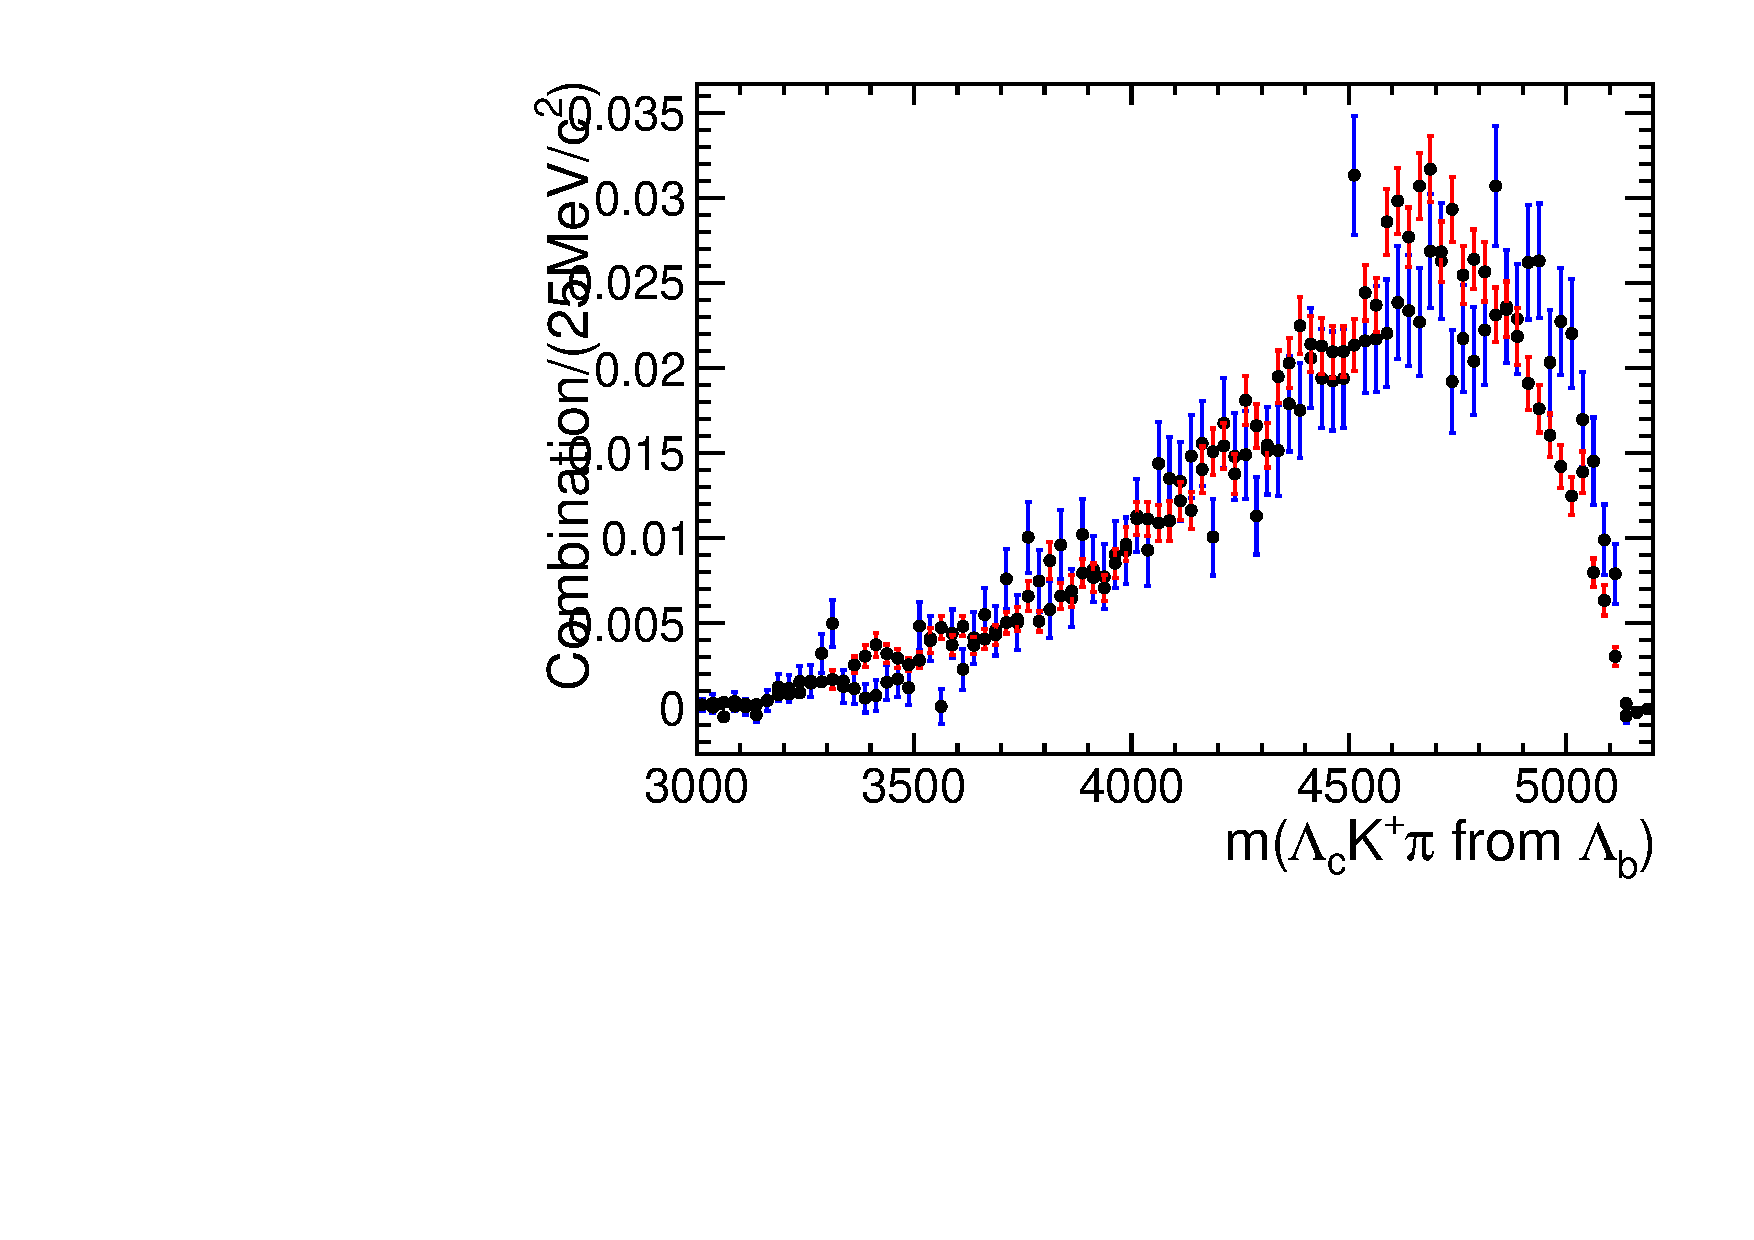
\includegraphics[width=0.4\textwidth]{Figures/05_open_charm/04_tune/new_for_note/LcLbKpPi_M_con.pdf}%
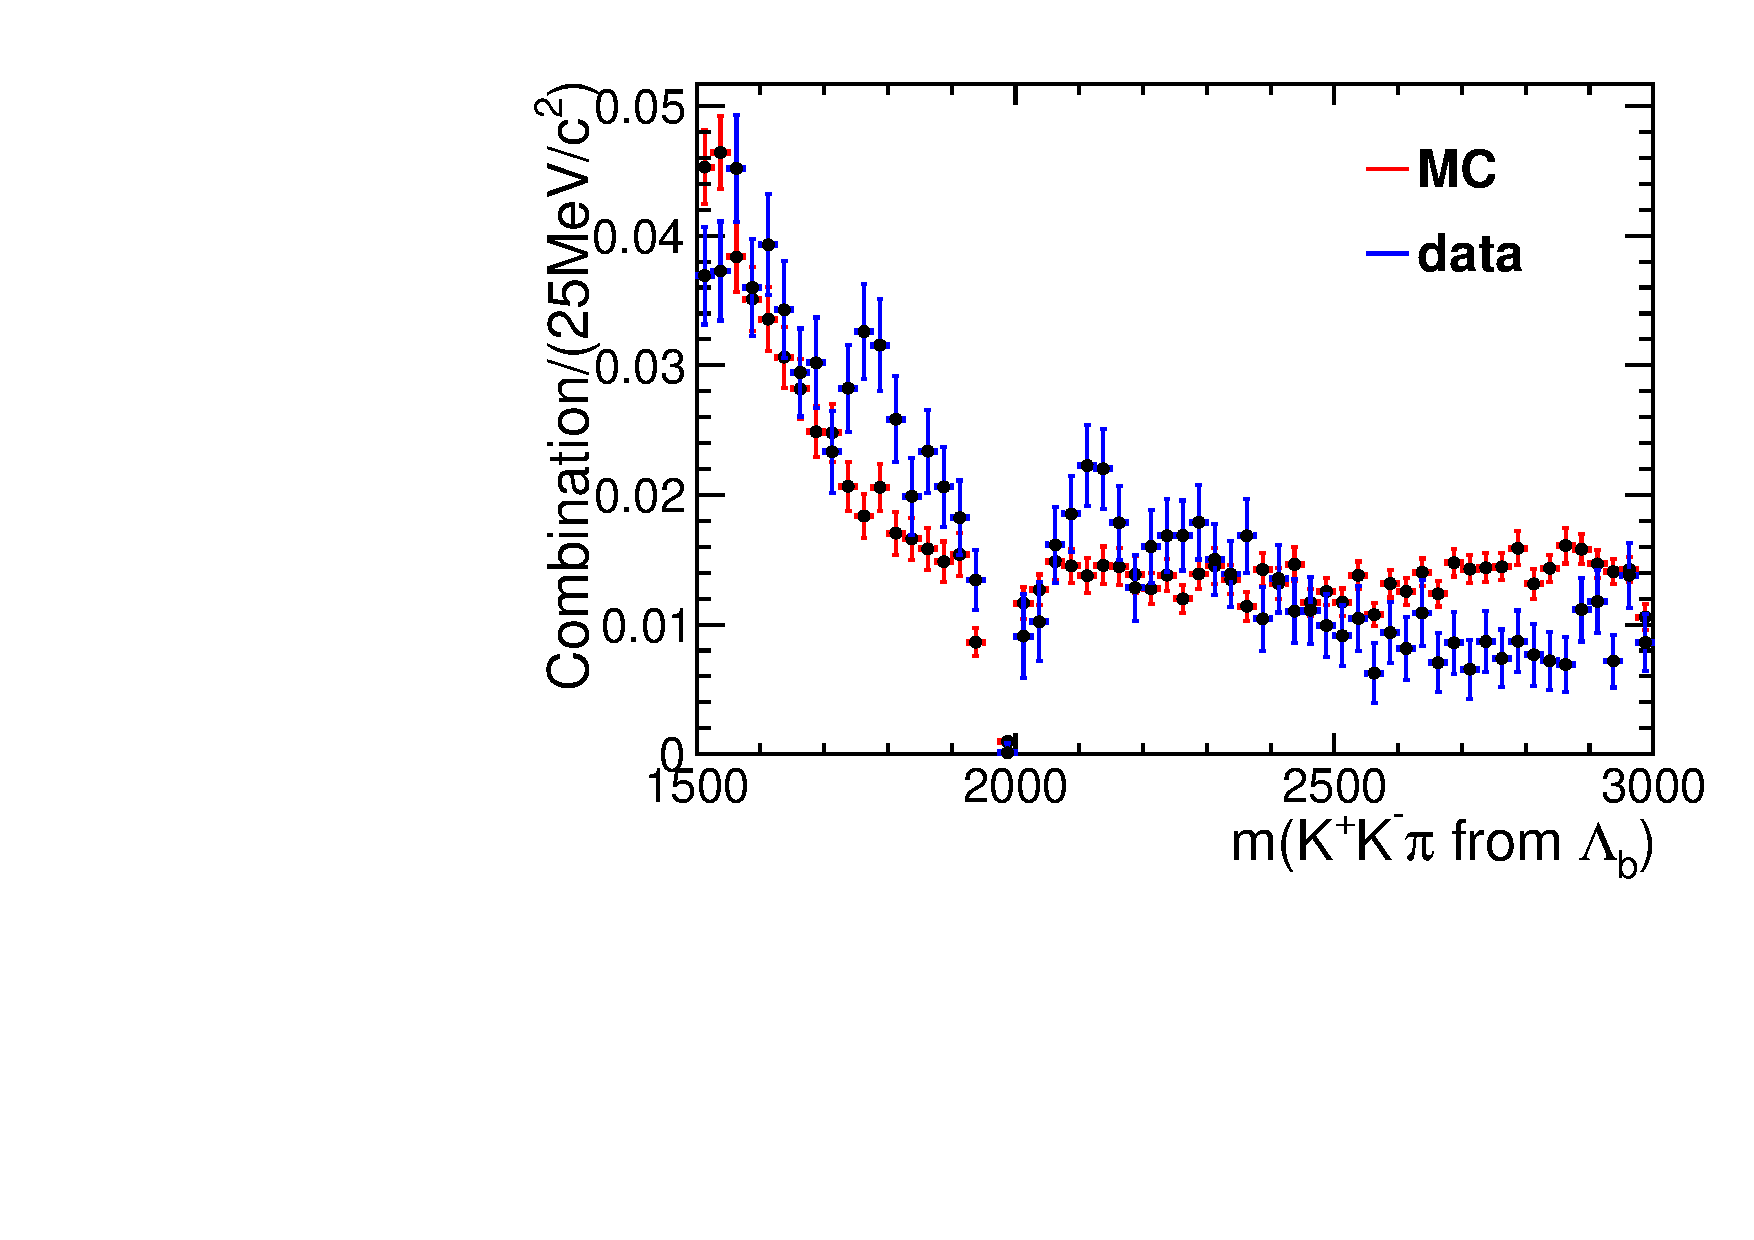
\includegraphics[width=0.4\textwidth]{Figures/05_open_charm/04_tune/new_for_note/LbKpKmPi_M.pdf}\\%
\caption{The invariant mass distribution of  three body combination for \LbLckkpi in the background subtracted data and MC.}
\label{fig.Resonance_3body}
\end{figure}  


Figure.~\ref{fig.Resonance_2body} and Figure~\ref{fig.Resonance_3body} show the combinations distribution between the data sample and blended MC sample. 
As we have employed some vetoes in mass spectrum of $K^+\pi^-$ and $K^+K^-\pi^-$, 
the bin's size used in the resonance weight is larger than the size of veto mass window, 
in this way, we can avoid the divide-by-zero errors. 

From the bottom left plot shown in the Figure.~\ref{fig.Resonance_2body}, 
a clear peak of $\Sigma_{c}$ appears in the mass spectrum of $\Lc\pim$, 
this disagreement might cause a deviate for the estimation of efficiency, 
so we considered this effect in the systematic uncertainty calculation. 

%Besides, the zoomed distribution is shown in Figure.~\ref{fig.zoom_LcPi}.   
%\begin{figure}[hbt]
%\centering
%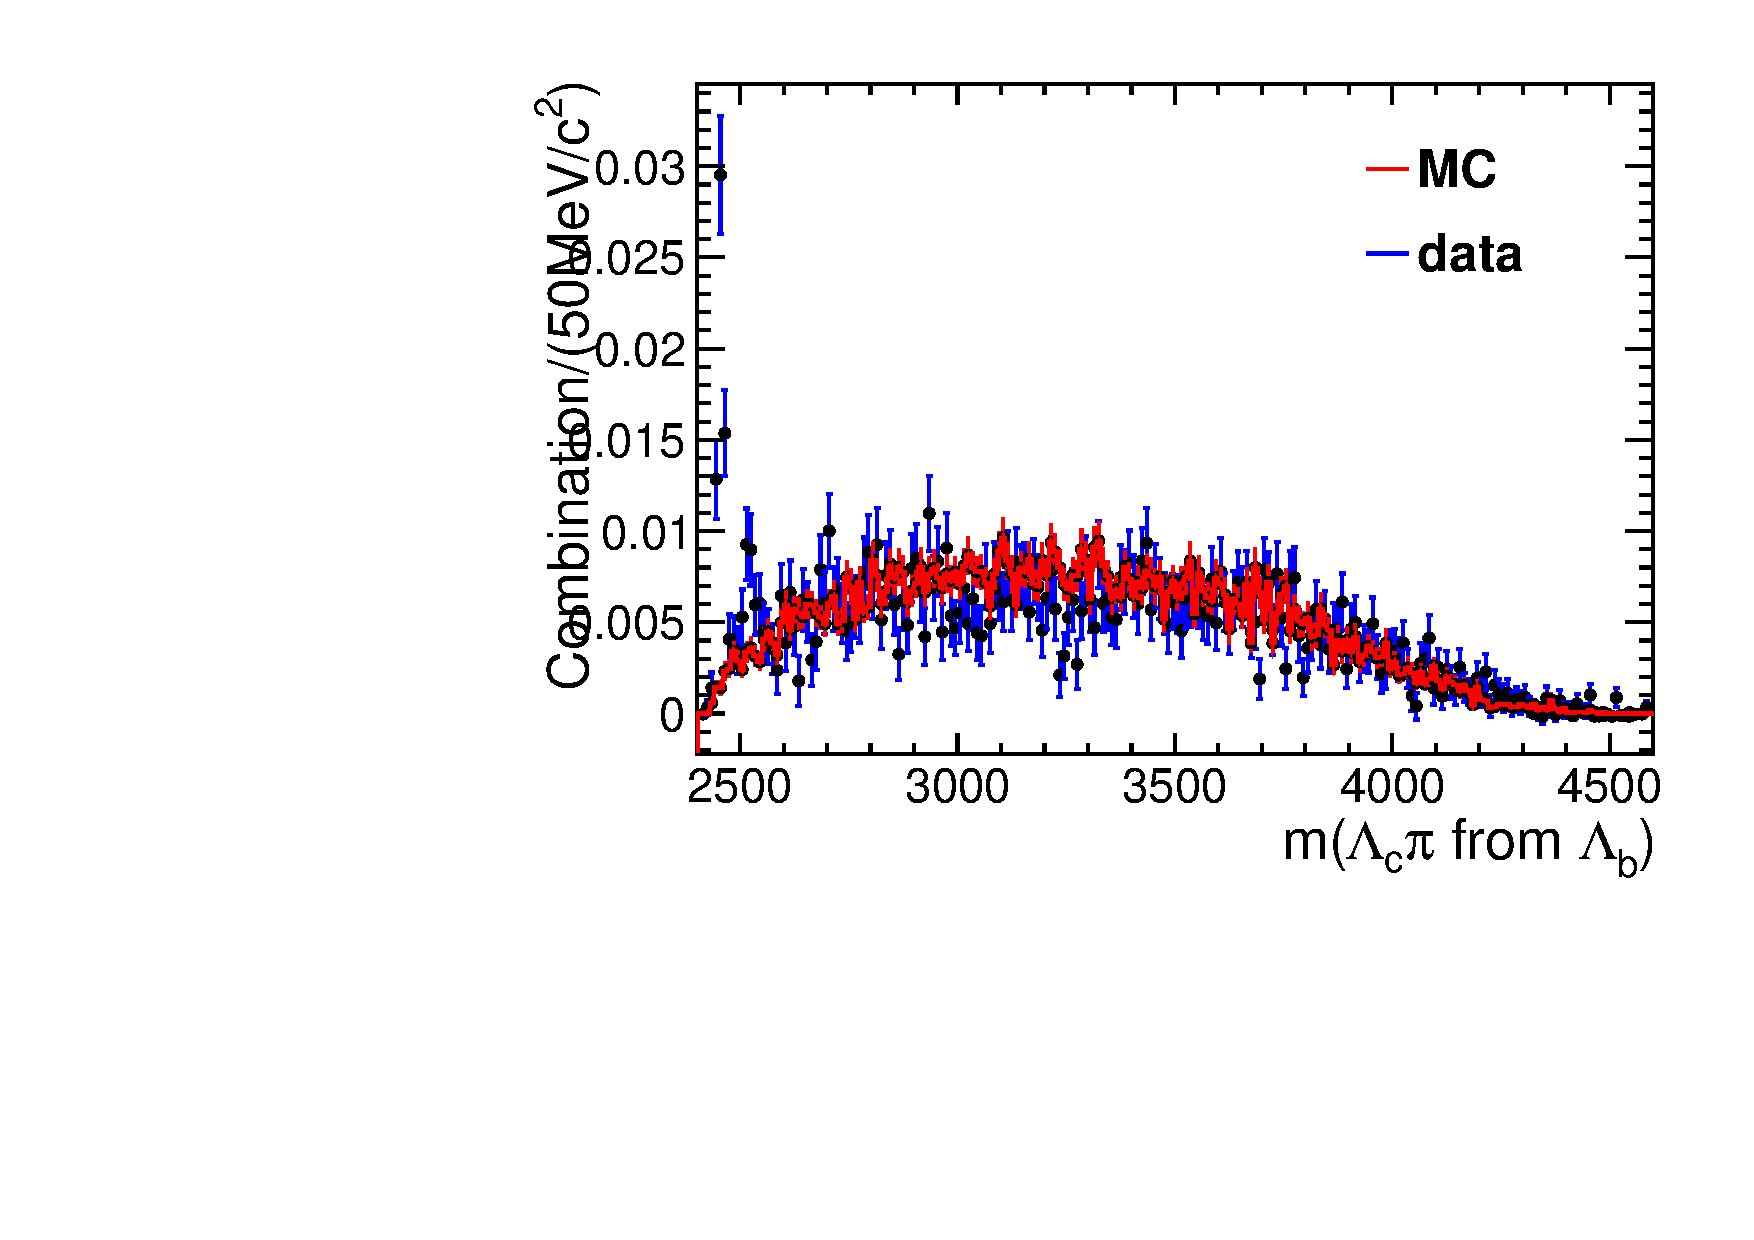
\includegraphics[width=0.5\textwidth]{plots/LcPi_zoom_in/LcLbPi_M_con.pdf}\\%
%\caption{The zoomed invariant mass distribution of $\Lc\pim$ combination for \LbLckkpi in the background subtracted data and MC.}
%\label{fig.zoom_LcPi}
%\end{figure}  


\subsection{Check the Reweight}
\label{sec:reweight_check}

We applied the $\pt,y$ weight, nTracks weight, \Lc dalitz weight and mass weight sequentially, 
with a weighting procedure performed on top of the previous weighting. 
In this case, 
we need to make sure the distributions weighted previously is not changed significantly by a later reweighting. 
So we need to check the distribution especially the first few weights. 
Some distributions after all weight are shown in Figure.~\ref{Fig.check_pi} and Figure.~\ref{Fig.check_kkpi}. 
All variables are consistent with each to a certain extent.
%more checks are shown in Appendix.~\ref{appendix:check}.

\begin{figure}[bth]
\centering
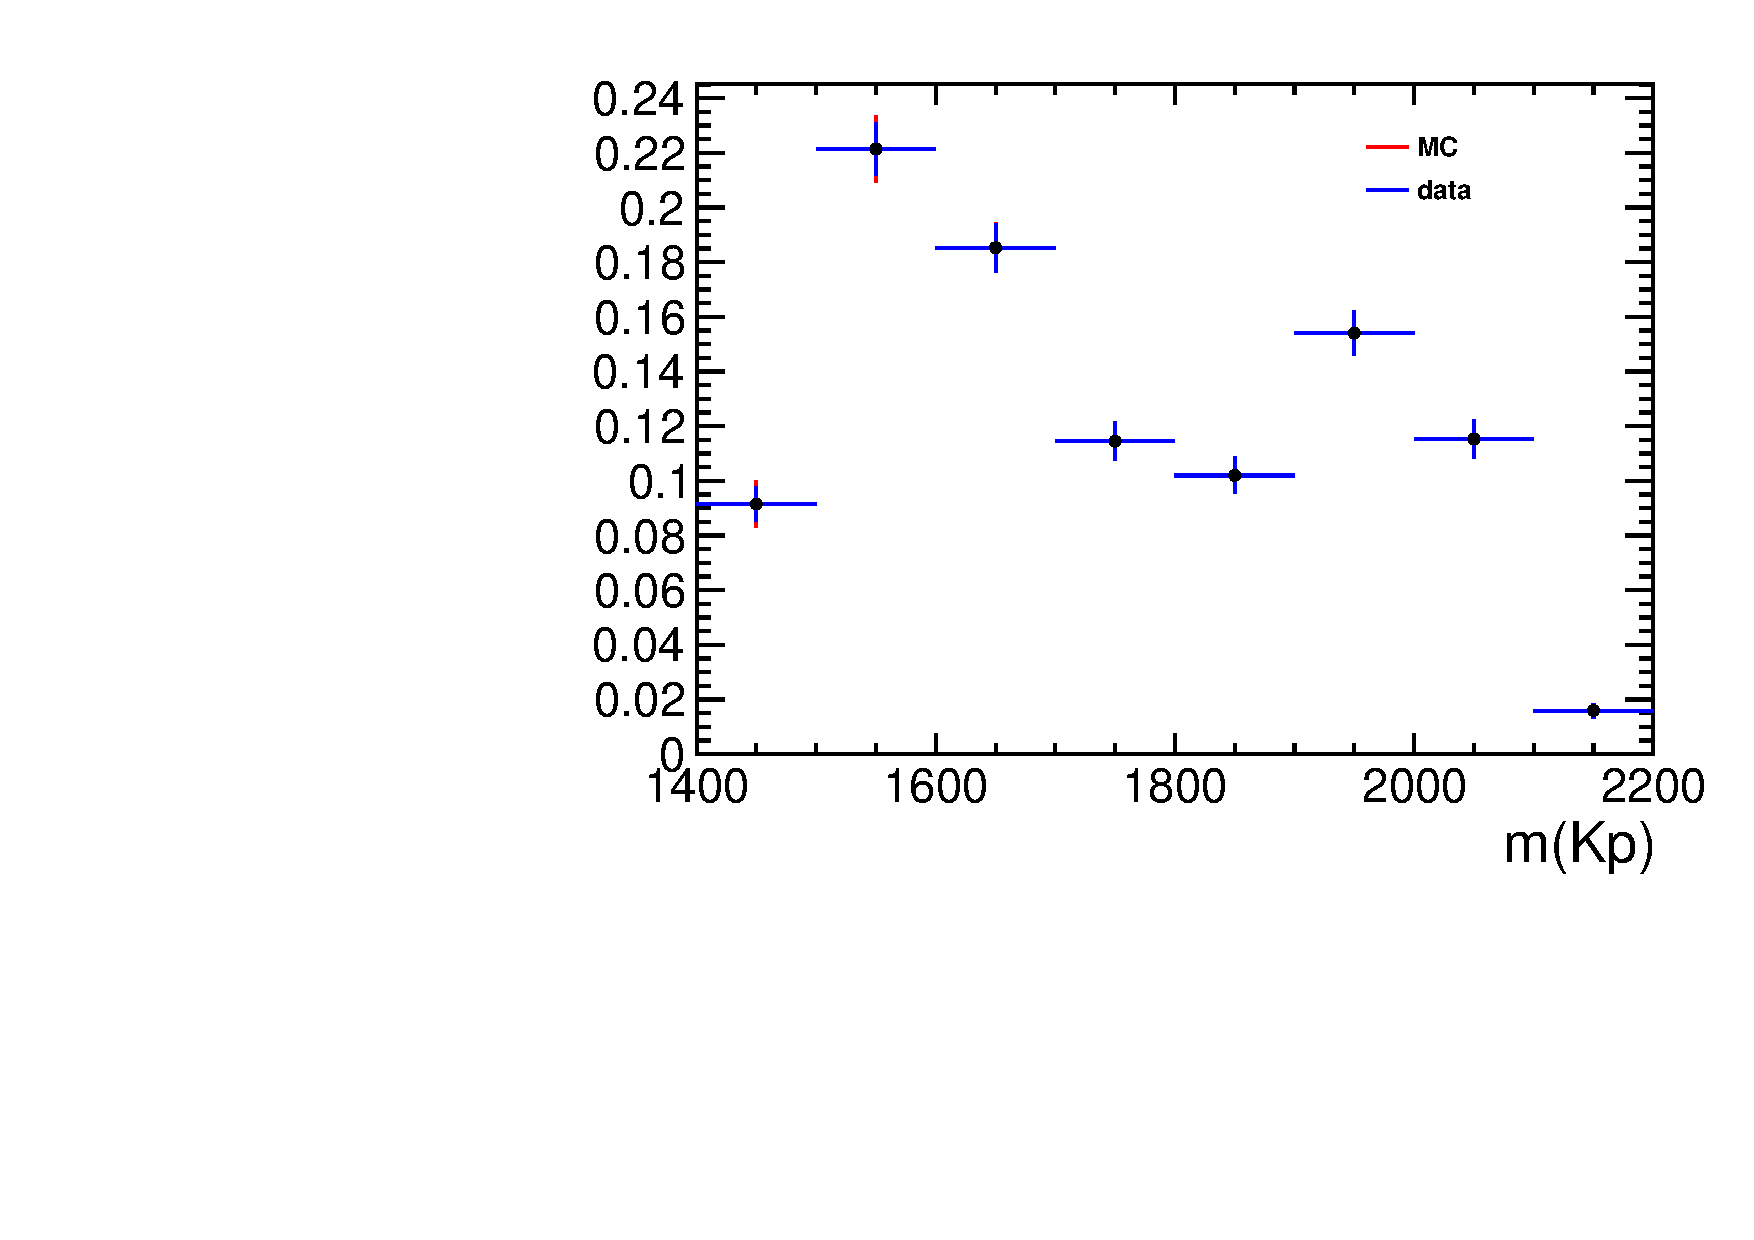
\includegraphics[width=0.4\textwidth]{Figures/05_open_charm/04_tune/after_weight_ds/mkp.pdf}%
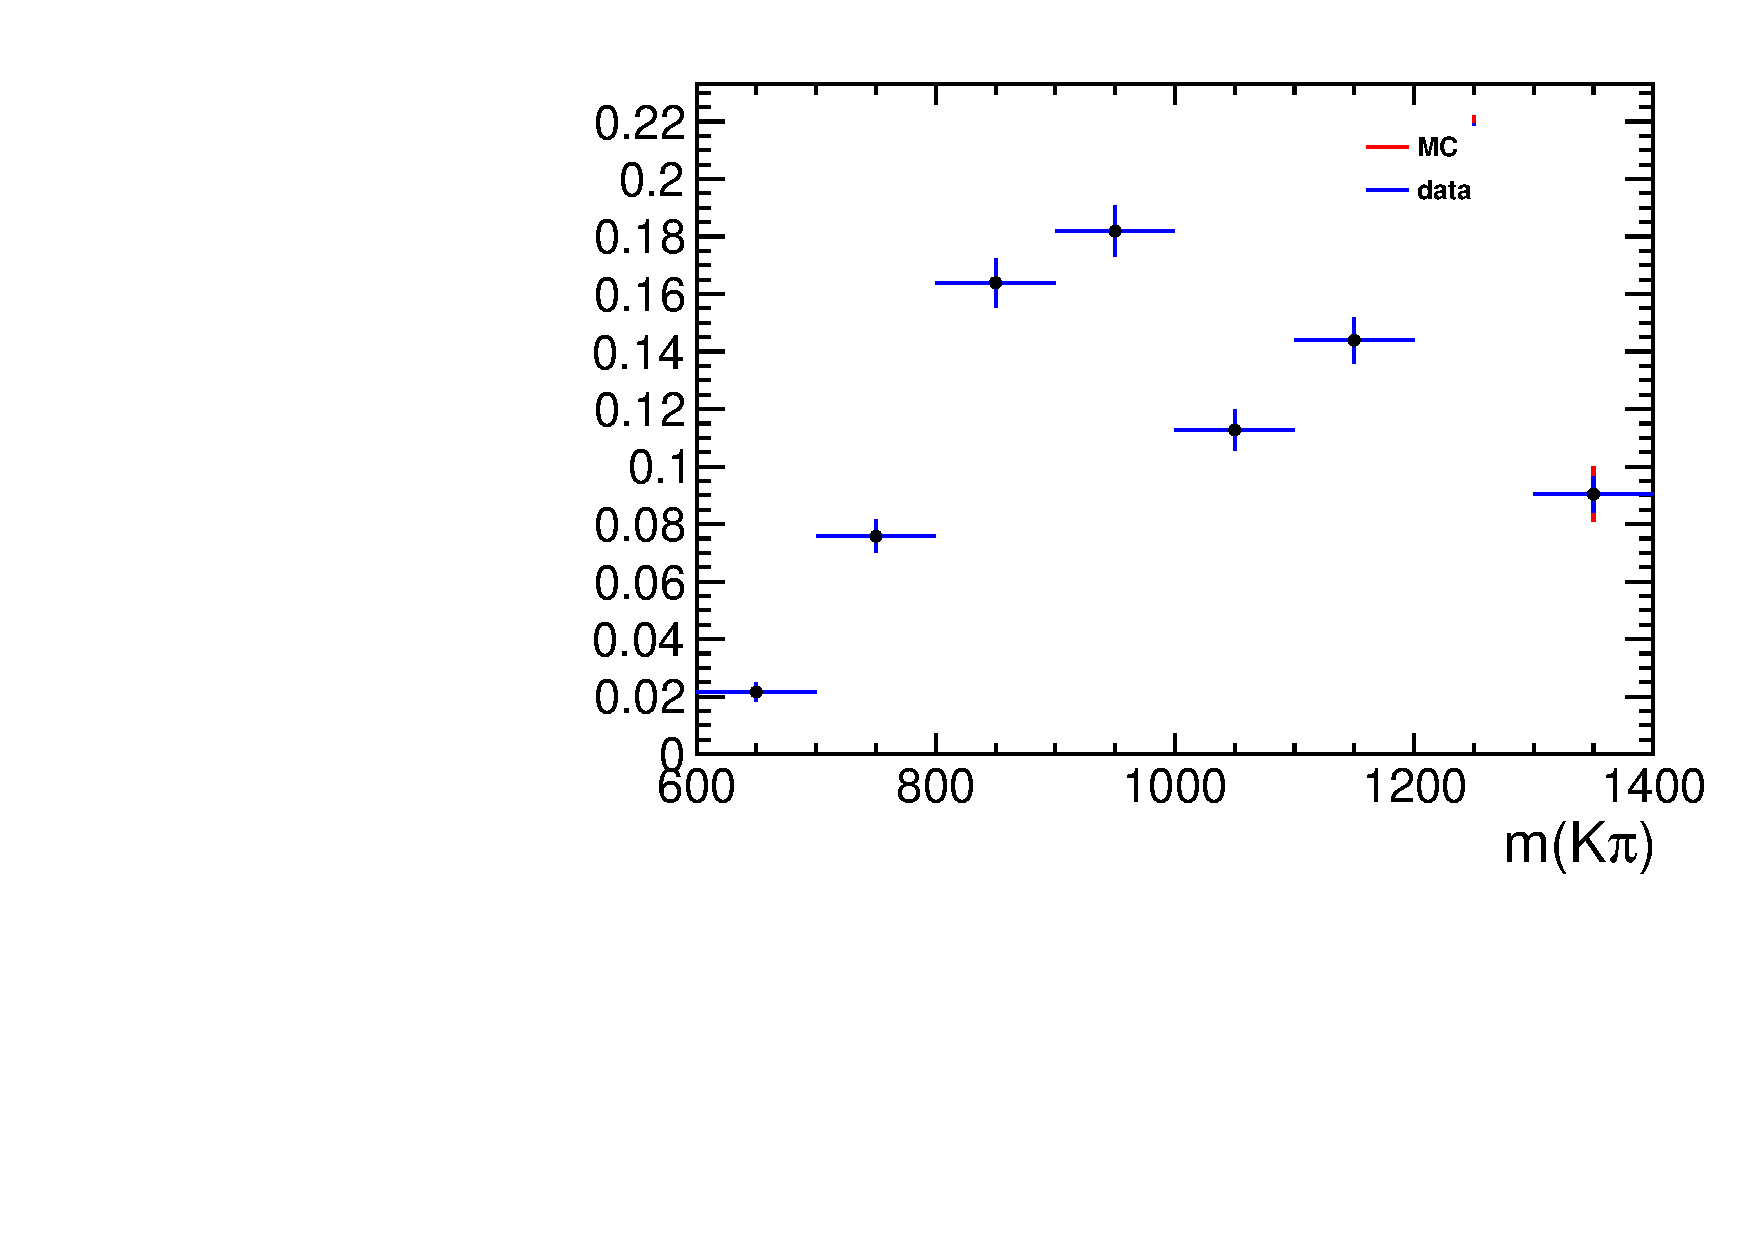
\includegraphics[width=0.4\textwidth]{Figures/05_open_charm/04_tune/after_weight_ds/mkpi.pdf}\\
\caption{Comparison of variables between background subtracted data and weighted MC in the \LbLcDs channel.}
\label{Fig.check_pi}
\end{figure}


\begin{figure}[bth]
\centering
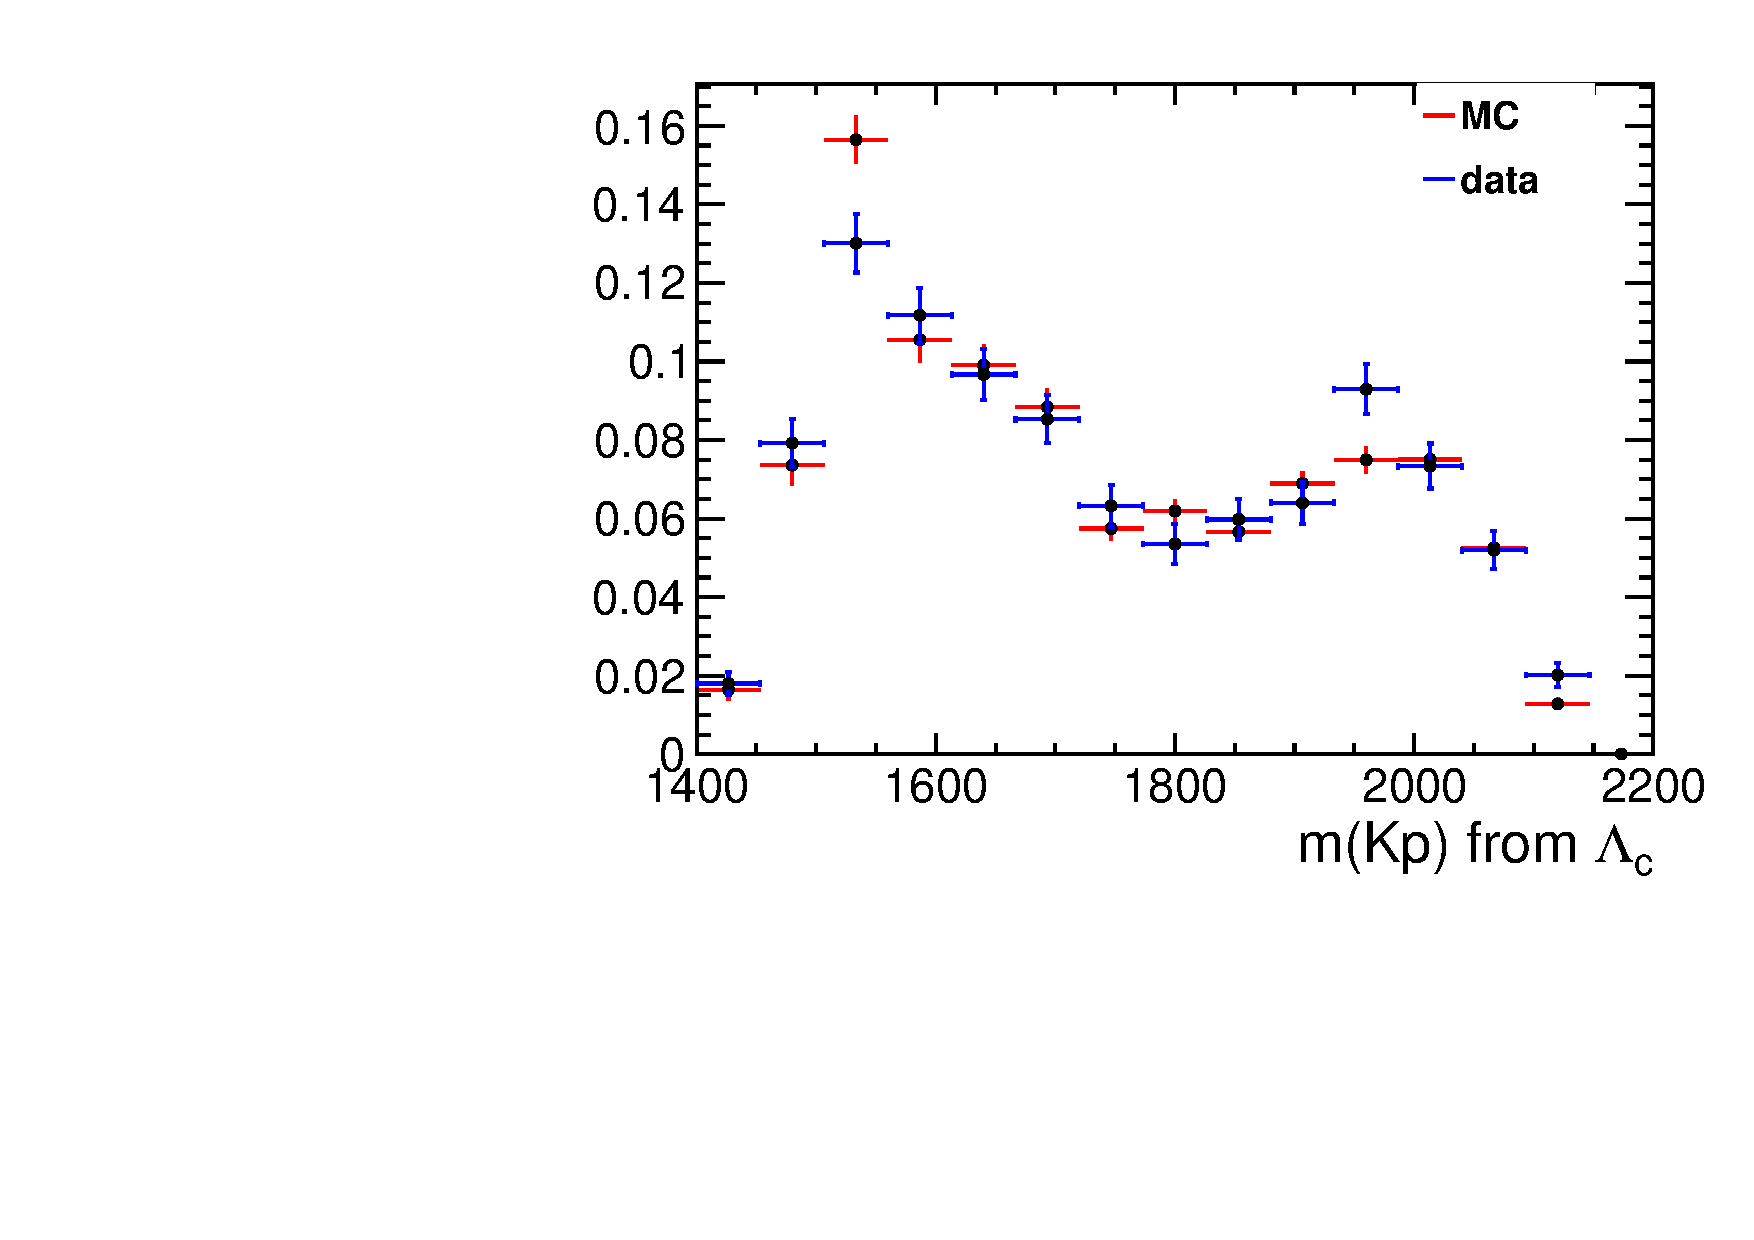
\includegraphics[width=0.4\textwidth]{Figures/05_open_charm/04_tune/after_weight_kkpi/mkp.pdf}%
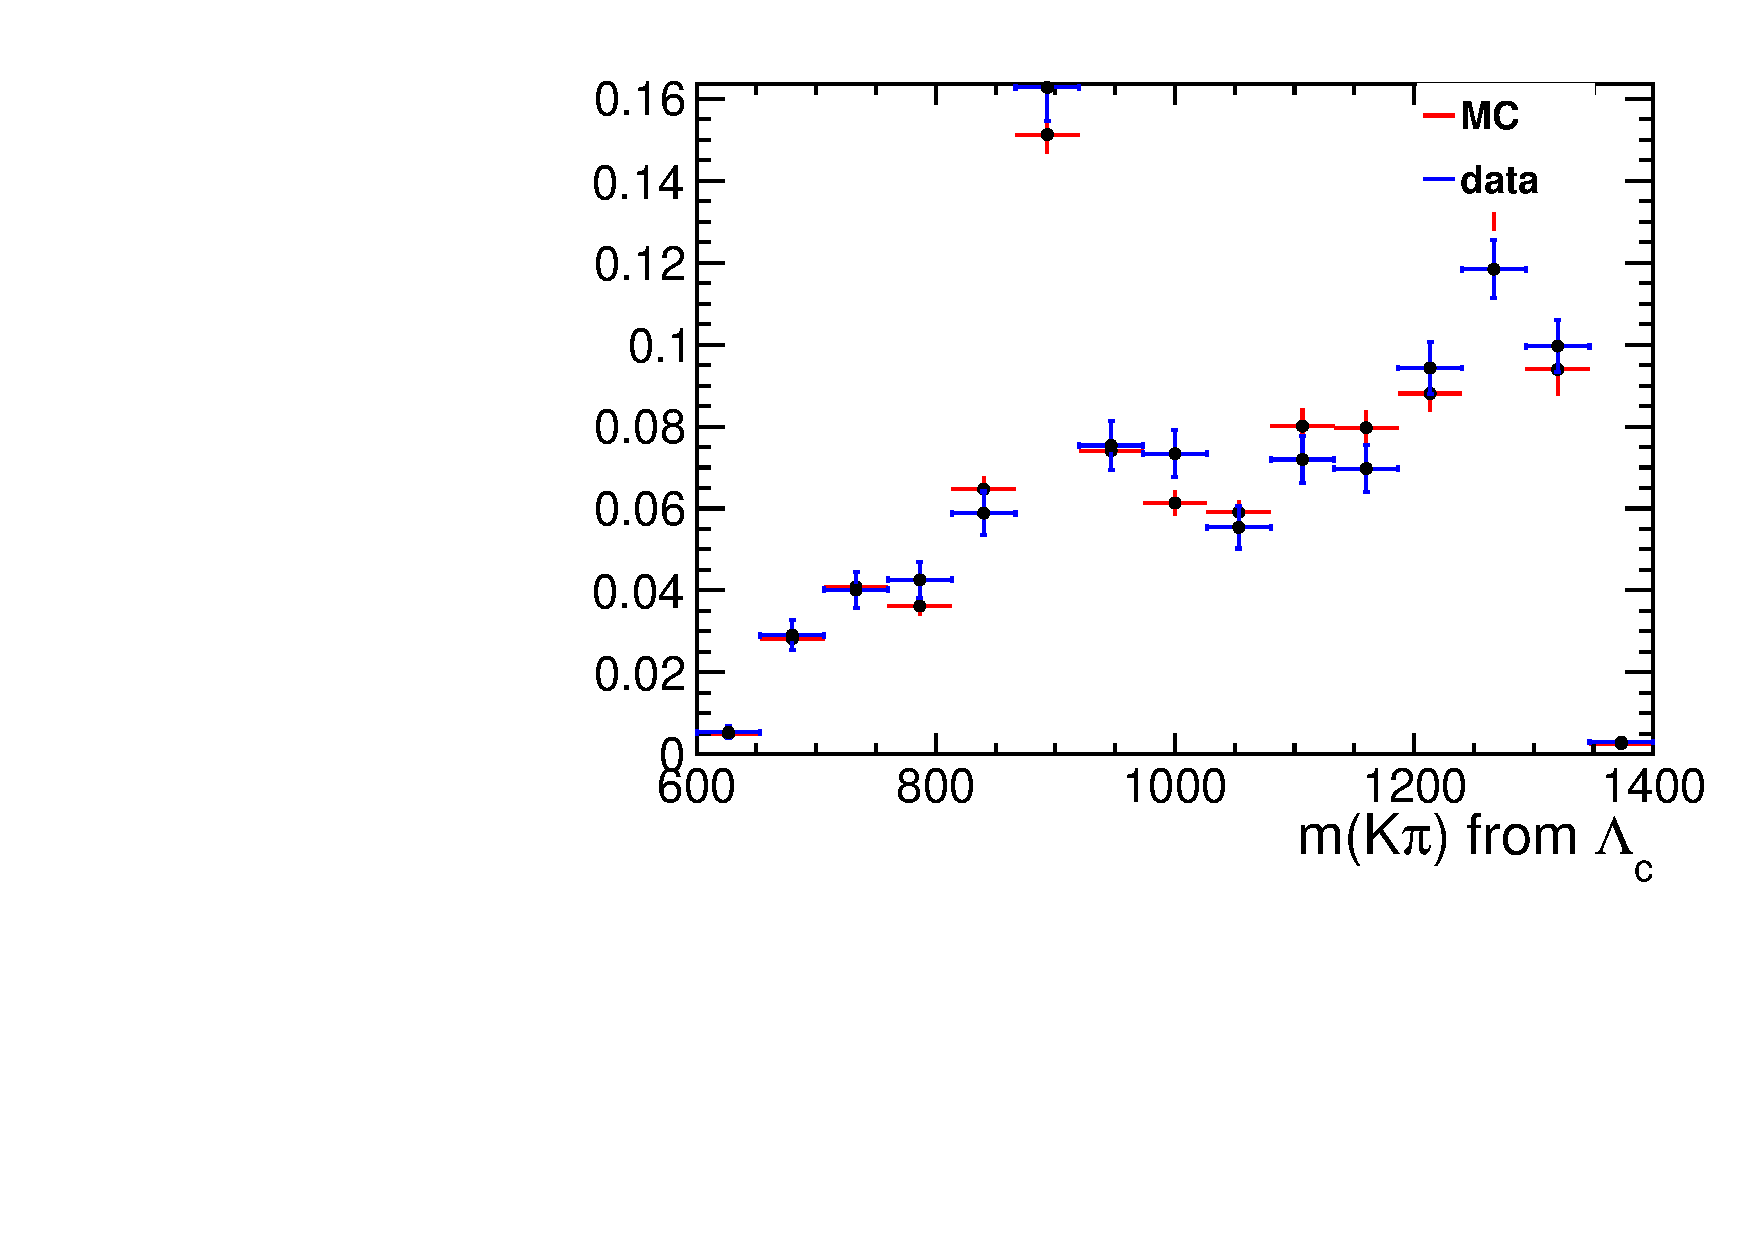
\includegraphics[width=0.4\textwidth]{Figures/05_open_charm/04_tune/after_weight_kkpi/mkpi.pdf}\\
	\caption{Comparison of variables between background subtracted data and weighted MC in the \LbLckkpi channel.}
\label{Fig.check_kkpi}
\end{figure}


